\section{Experiments}
There are a number of different axes on which we can evaluate \sys.
First, we take real datasets and generate various types of errors to illustrate the value of data cleaning in comparison to robust statistical techniques.
Next, we explore different prioritization and model update schemes for data cleaning samples.
Finally, we evaluate \sys end-to-end in a number of real-world data cleaning scenarios.

\subsection{Experimental Setup and Notation}
Our main metric for evaluation is a relative measure of trained model with \sys (or an alternative technique) and the model if all of the data is cleaned.

\vspace{0.25em}

\noindent\textbf{Relative Model Error. } Let $\theta$ be the model trained on the dirty data, and let $\theta^*$ be the model trained on the same data if it was cleaned. Then the model error is defined as $\frac{\|\theta - \theta^*\|}{\|\theta^*\|}$.

\subsubsection{Scenarios}
\noindent We apply \sys to the following scenarios:

%\vspace{0.5em}

%\noindent\textbf{Housing: } In this dataset, our task is to predict housing prices from 13 numerical and categorical covariates. There are 550 data points in this dataset. The model is a Logistic Regression classifier which predicts if the house price is greater than \$500k.

\vspace{0.25em}

\noindent\textbf{Income Classification (Adult): } In this census dataset, our task is to predict the income bracket (binary) from 12 numerical and categorical covariates. There are 45552 data points in this dataset. We use a SVM classifier to predict the income bracket of the person.

\vspace{0.25em}

\noindent\textbf{Seizure Classification (EEG): } In this dataset, our task is to predict the on set of a seizure (binary) from 15 numerical covariates. There are 14980 data points in this dataset. We chose this dataset since the classification task is hard with an accuracy in clean data of 65\%. The model that we use is a thresholded Linear Regression.

\vspace{0.25em}

\noindent\textbf{Handwriting Recognition (MNIST): } In this dataset, our task is to classify 60,000 images of handwritten images into 10 categories. The unique part of this dataset is the featurized data consists of a 784 dimensional vector which includes edge detectors and raw image patches. We use this dataset to explore how we can corrupt the raw data to affect subsequent featurization. The model is an one-to-all multiclass SVM classifier. 

\vspace{0.25em}

\noindent\textbf{Dollars For Docs: } We introduced this dataset earlier in the paper, and here we highlight some of the details. The dataset has 240089 records with 5 textual attributes and one numerical attribute.
We used a bag-of-words featurization model for the textual attributes which resulted in a 2021 dimensional feature vector. 
We use this feature vector via a binary SVM to classify whether a research contribution is ``not covered" under the declared experimental protocal from the attributes.

\subsubsection{Compared Algorithms}
\noindent Here are the alternative methodologies that we consider:

\vspace{0.25em}

\noindent\textbf{Robust Logistic Regression \cite{feng2014robust}. } Feng et al. proposed a variant of logistic regression that is robust to outliers. We chose this algorithm because it is a robust extension of the convex regularized loss model, leading to a better apples-to-apples comparison between the techniques. (See details in Appendix \ref{rlogit})  

\vspace{0.25em}

\noindent\textbf{Discarding Dirty Data. } As a baseline we explore model accuracy when dirty data is discarded.

\vspace{0.25em}

\noindent\textbf{SampleClean (SC) \cite{wang1999sample}. } In SampleClean, we take a sample of data, apply data cleaning, and then train a model to completion.

\vspace{0.25em}

\noindent\textbf{Active Learning (AL) \cite{guillory2009active}. } We compare against an Active Learning algorithm that integrates with stochastic optimization (See details in Appendix \ref{al}). 

\vspace{0.25em}

\noindent\textbf{ActiveClean Oracle (AC+O): } In \sys Oracle, we importance sample points by their clean gradient. This represents the theoretical best that our algorithm could hope to achieve given perfect estimation.

\subsection{Does Data Cleaning Matter?}
Before we evaluate \sys, we first evaluate the benefits of cleaning on 2 of our example datasets (EEG and Adult).
We first explore this problem without sampling to understand which types of data corruption are amenable to data cleaning and which are better suited for robust statistical techniques.
We compare 4 schemes: (1) full data cleaning uncorrupted, (2) baseline of no cleaning, (3) discarding the dirty data, and (4) robust logistic regression,. We corrupted 5\% of the training examples in each dataset in two different ways:

\vspace{0.5em}

\noindent\textbf{Random Corruption: } We simulated high-magnitude random outliers. We select 5\% of the examples and features uniformly at random and replace a feature with 3 times the highest feature value.

\vspace{0.5em}

\noindent\textbf{Systematic Corruption: } We simulated innocuous looking (but still incorrect) systematic corruption. We trained the model on the clean data, find the three most important feature (highest weighted). We sort examples by each these features and corrupt the top of examples with the mean value for that feature. 
At the end, we have corrupted 5\% of the examples.
It is important to note the some examples can have multiple corrupted features.

\begin{figure}[ht!]
\centering
 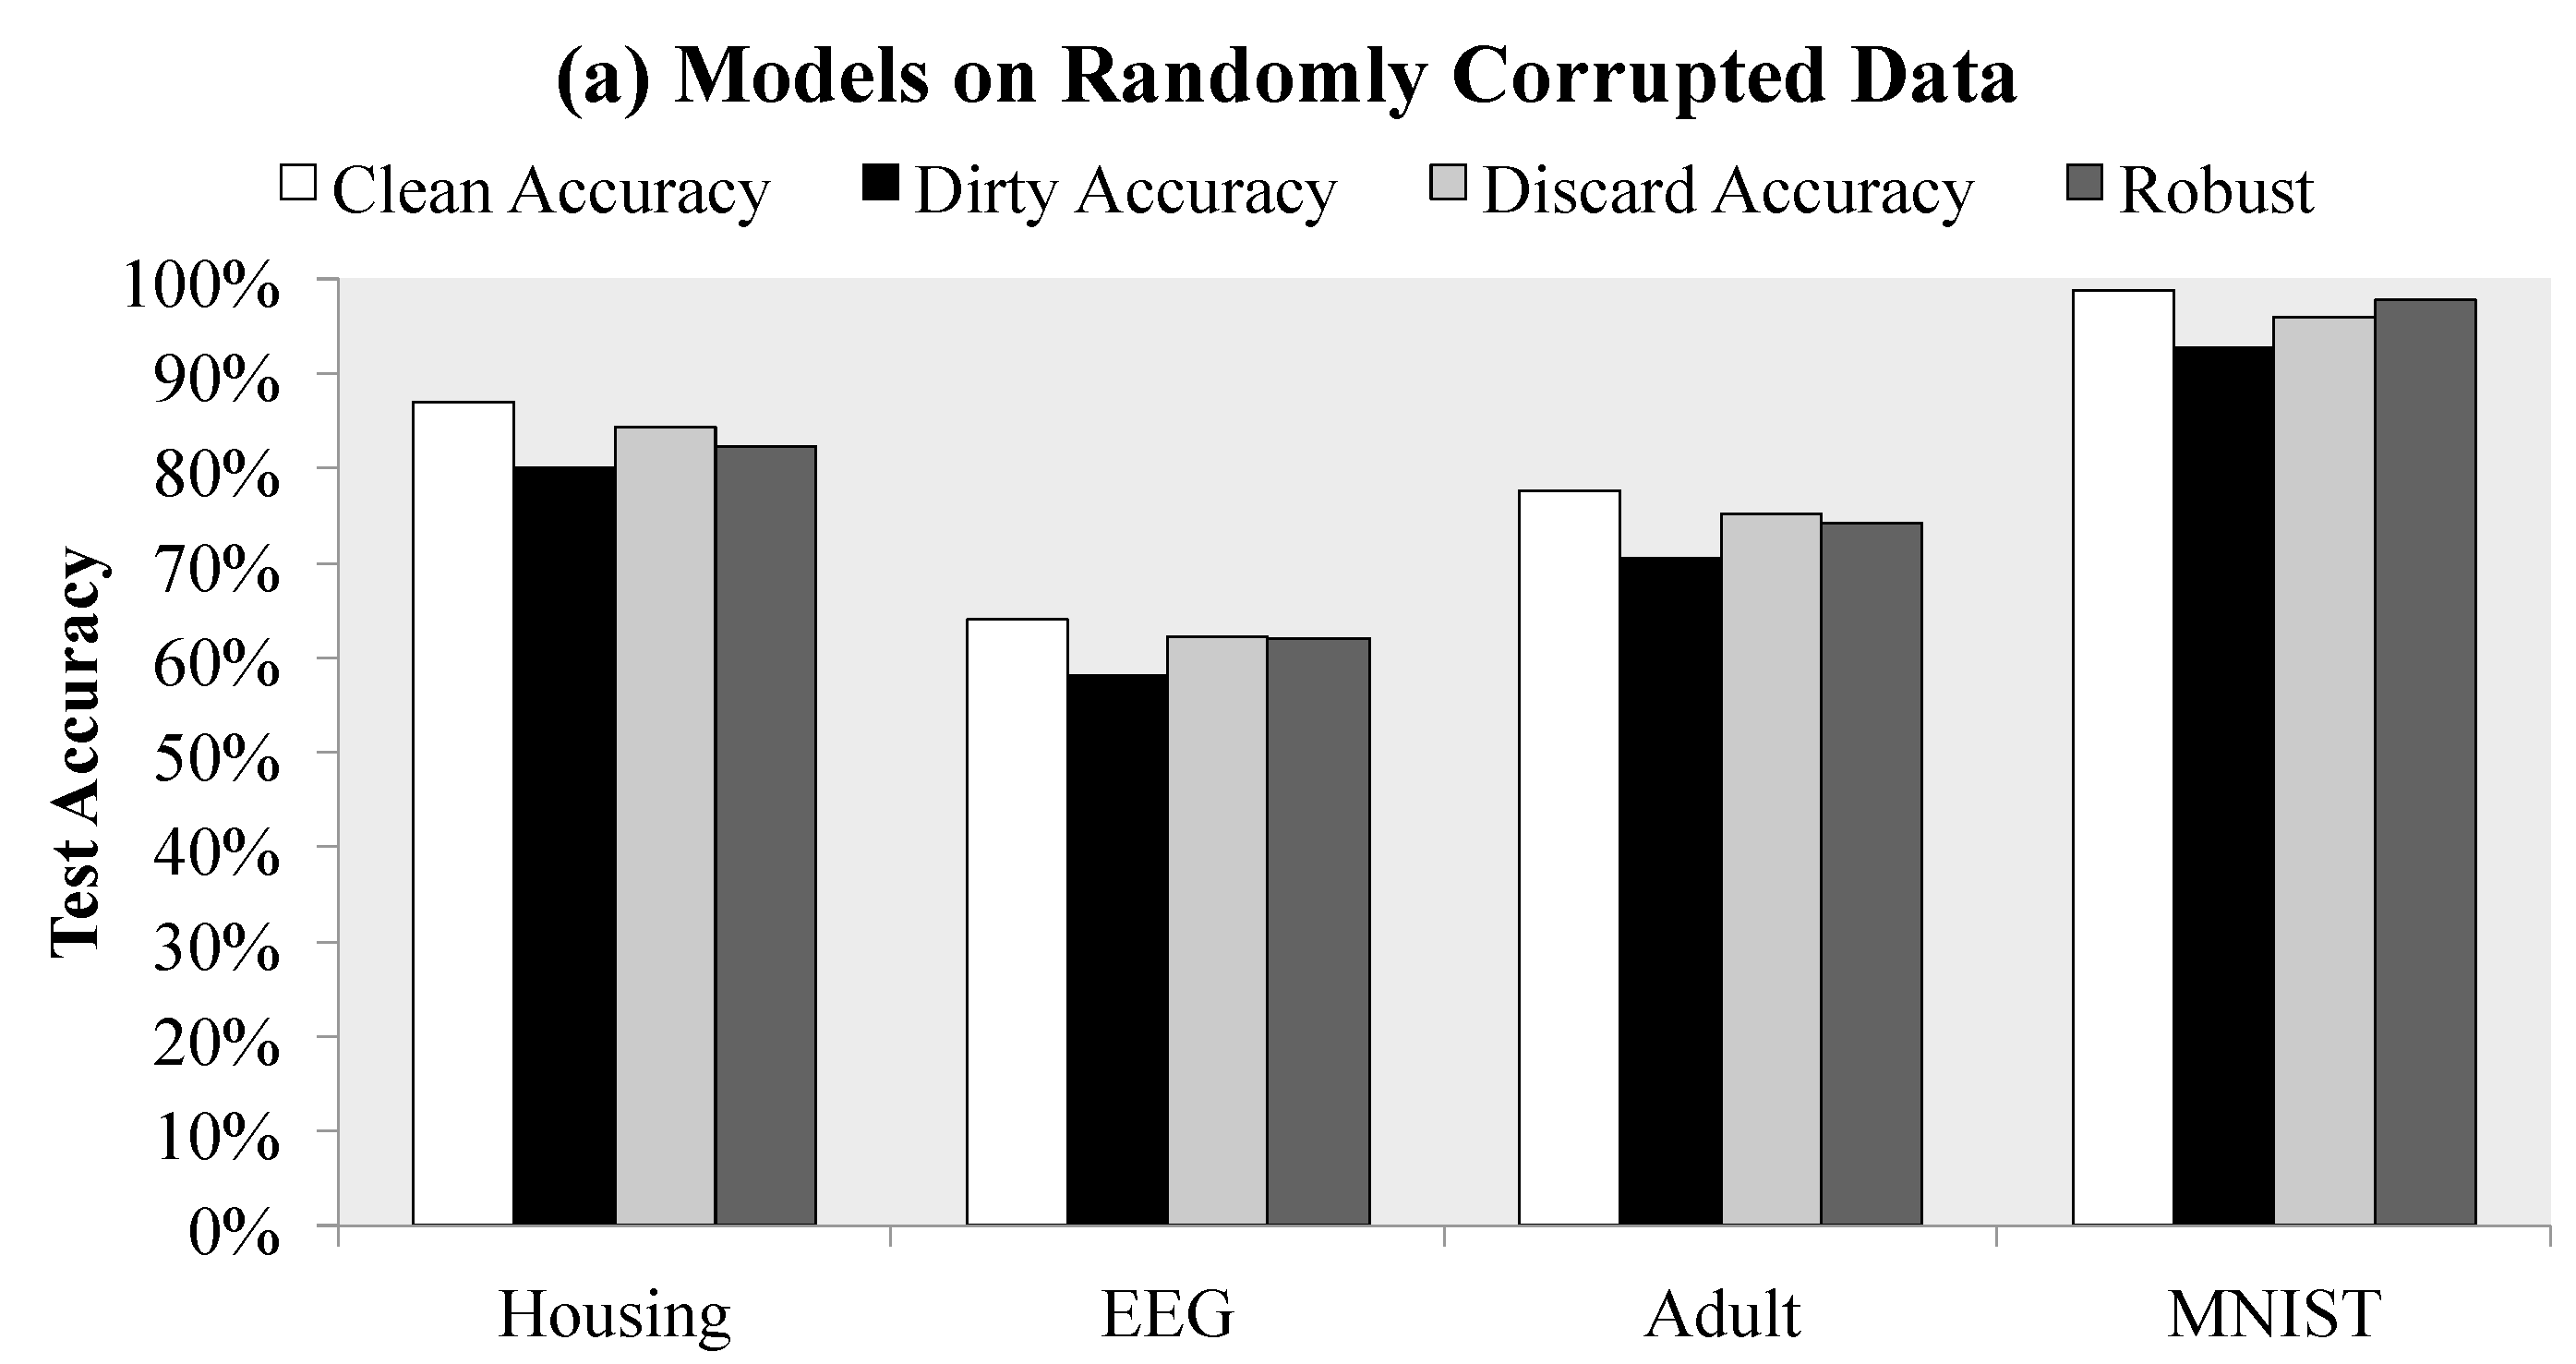
\includegraphics[width=0.49\columnwidth]{exp/exp2.pdf}
 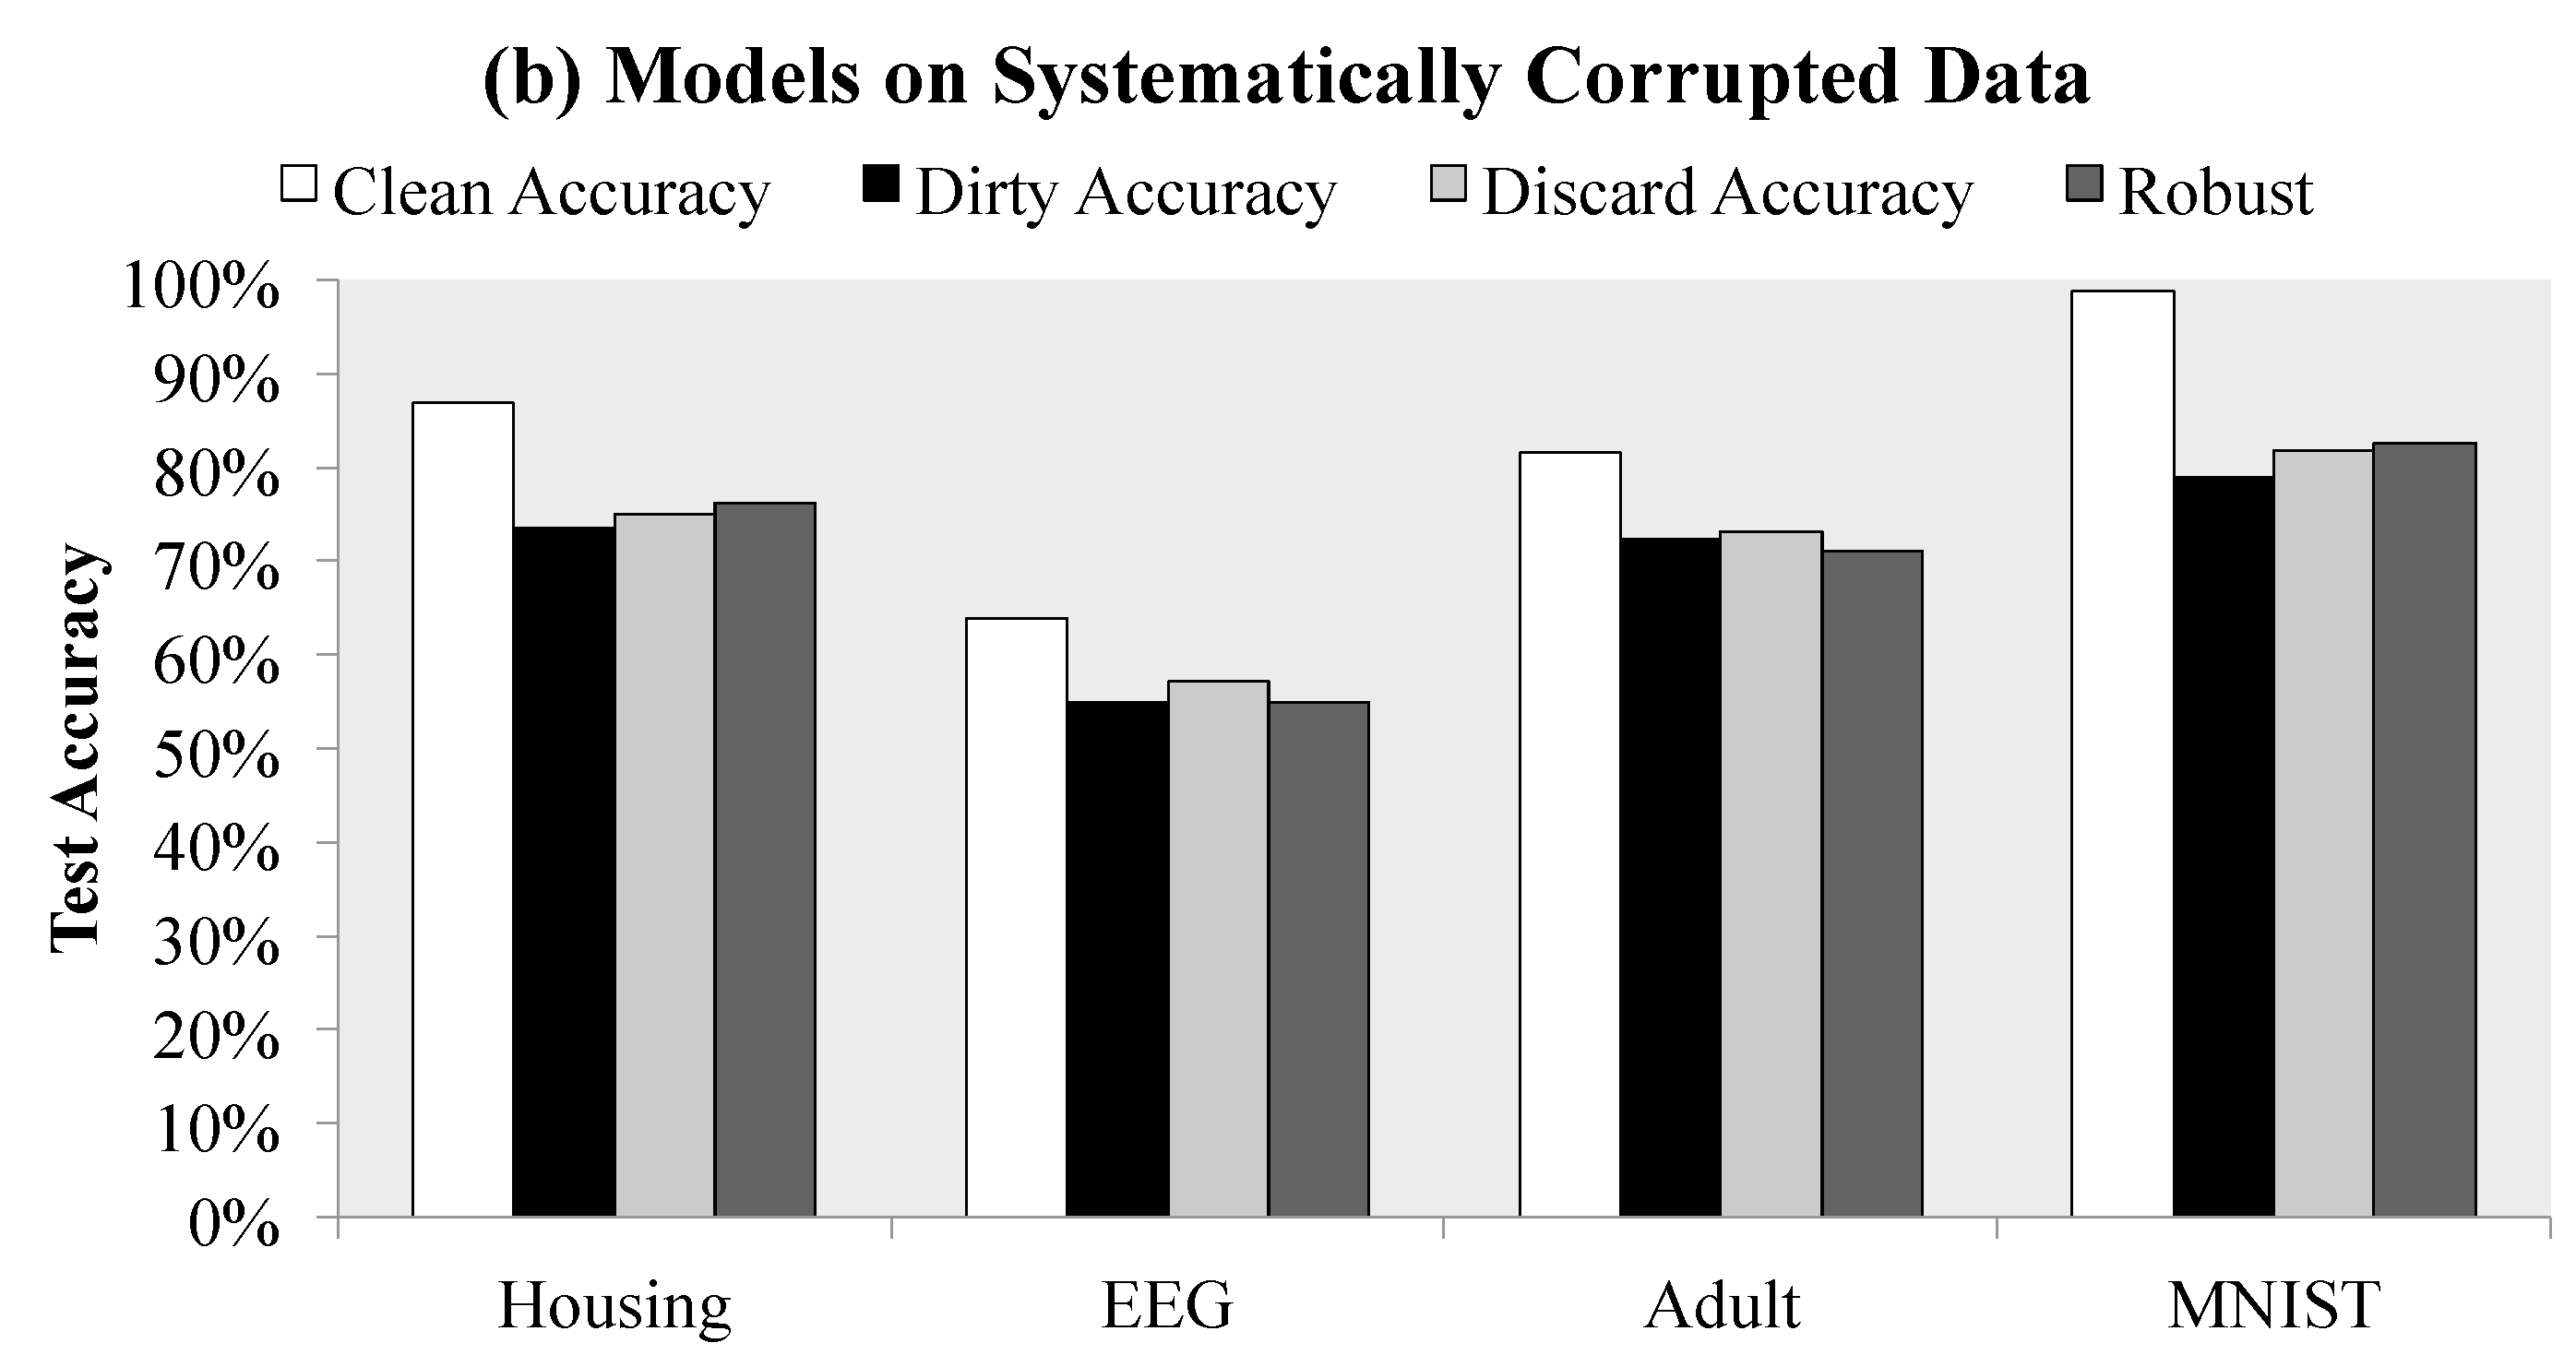
\includegraphics[width=0.49\columnwidth]{exp/exp1.pdf}
 \caption{(a) Robust techniques and discarding data work when corrupted data are random and look atypical. (b) Data cleaning can provide reliable performance in both the systematically corrupted setting and randomly corrupted setting.\label{sys-rand}}
\end{figure}

We plot the test accuracy for models trained on both types of data with the different techniques, since it is a binary classification task with balanced class distributions we cut the plots at 50\% (random accuracy) (Figure \ref{sys-rand}).
As we argued in this paper, the robust method performs well on the random high-magnitude outliers, however, falters on the systematic corruption.
In the random setting, discarding dirty data also performs well.
However, when the corruption is systematic, neither alternative works.
Data cleaning is the most reliable option across datasets and corruption types.
The problem is that without cleaning we do not know if the corruption is random or systematic.
While data cleaning requires more effort, it provides benefits in both settings.
In the remaining experiments, unless otherwise noted, we use the systematic corruption.

\vspace{0.25em}

\noindent \emph{Summary: Data cleaning mitigates the effects of both systematic and random corruption.}

\subsection{\sys A Priori Detection}
The next set of experiments evaluate different approaches to cleaning a sample of data.
In this set of experiments, we use the \emph{a priori} case for detection.
We assume that we know all of the corrupted records in advance but do not know how to repair them. 

\subsubsection{Comparison with Active Learning and SampleClean}
In our first experiment, we evaluate the samples-to-error tradeoff between three alternative algorithms: \sys (AC), SampleClean, Active Learning, and \sys+Oracle (AC+O).
In Figure \ref{prio-perf}, we present our results on Adult and EEG. 
We find that \sys gives its largest benefits for small sample sizes (up-to 12x more accurate than SampleClean).
\sys makes significant progress because of its intelligent initialization, iterative updates, and partitioning.
For example, the EEG dataset is the hardest classification task.
SampleClean has difficulty on this dataset since it takes a uniform sample of data (only 5\% of which are corrupted on average) and tries to train a model using only this data.
\sys and Active Learning leverage the initialization from the dirty data to get an improved result. 
However, \sys and Active Learning differ in the way they prioritize cleaning.
Active Learning prioritizes with respect to a dirty model (i.e., is agnostic to data error) and \sys uses estimation and detection.
\sys's estimates and detection allow us to beat Active Learning on all three of the datasets.
\sys also is relatively close in performance to the oracular version (theoretical optimum).

However, to an end user the metric that matters is test accuracy.
In Figure \ref{prio-perf}, we present the results for the two datasets: Adult and EEG.
We find that in both Adult and EEG, \sys converges to clean test accuracy faster than the alternatives.

\vspace{0.25em}

\noindent \emph{Summary: \sys with a priori detection converges faster than SampleClean and Active Learning.}

\begin{figure}[ht!]
\centering
 %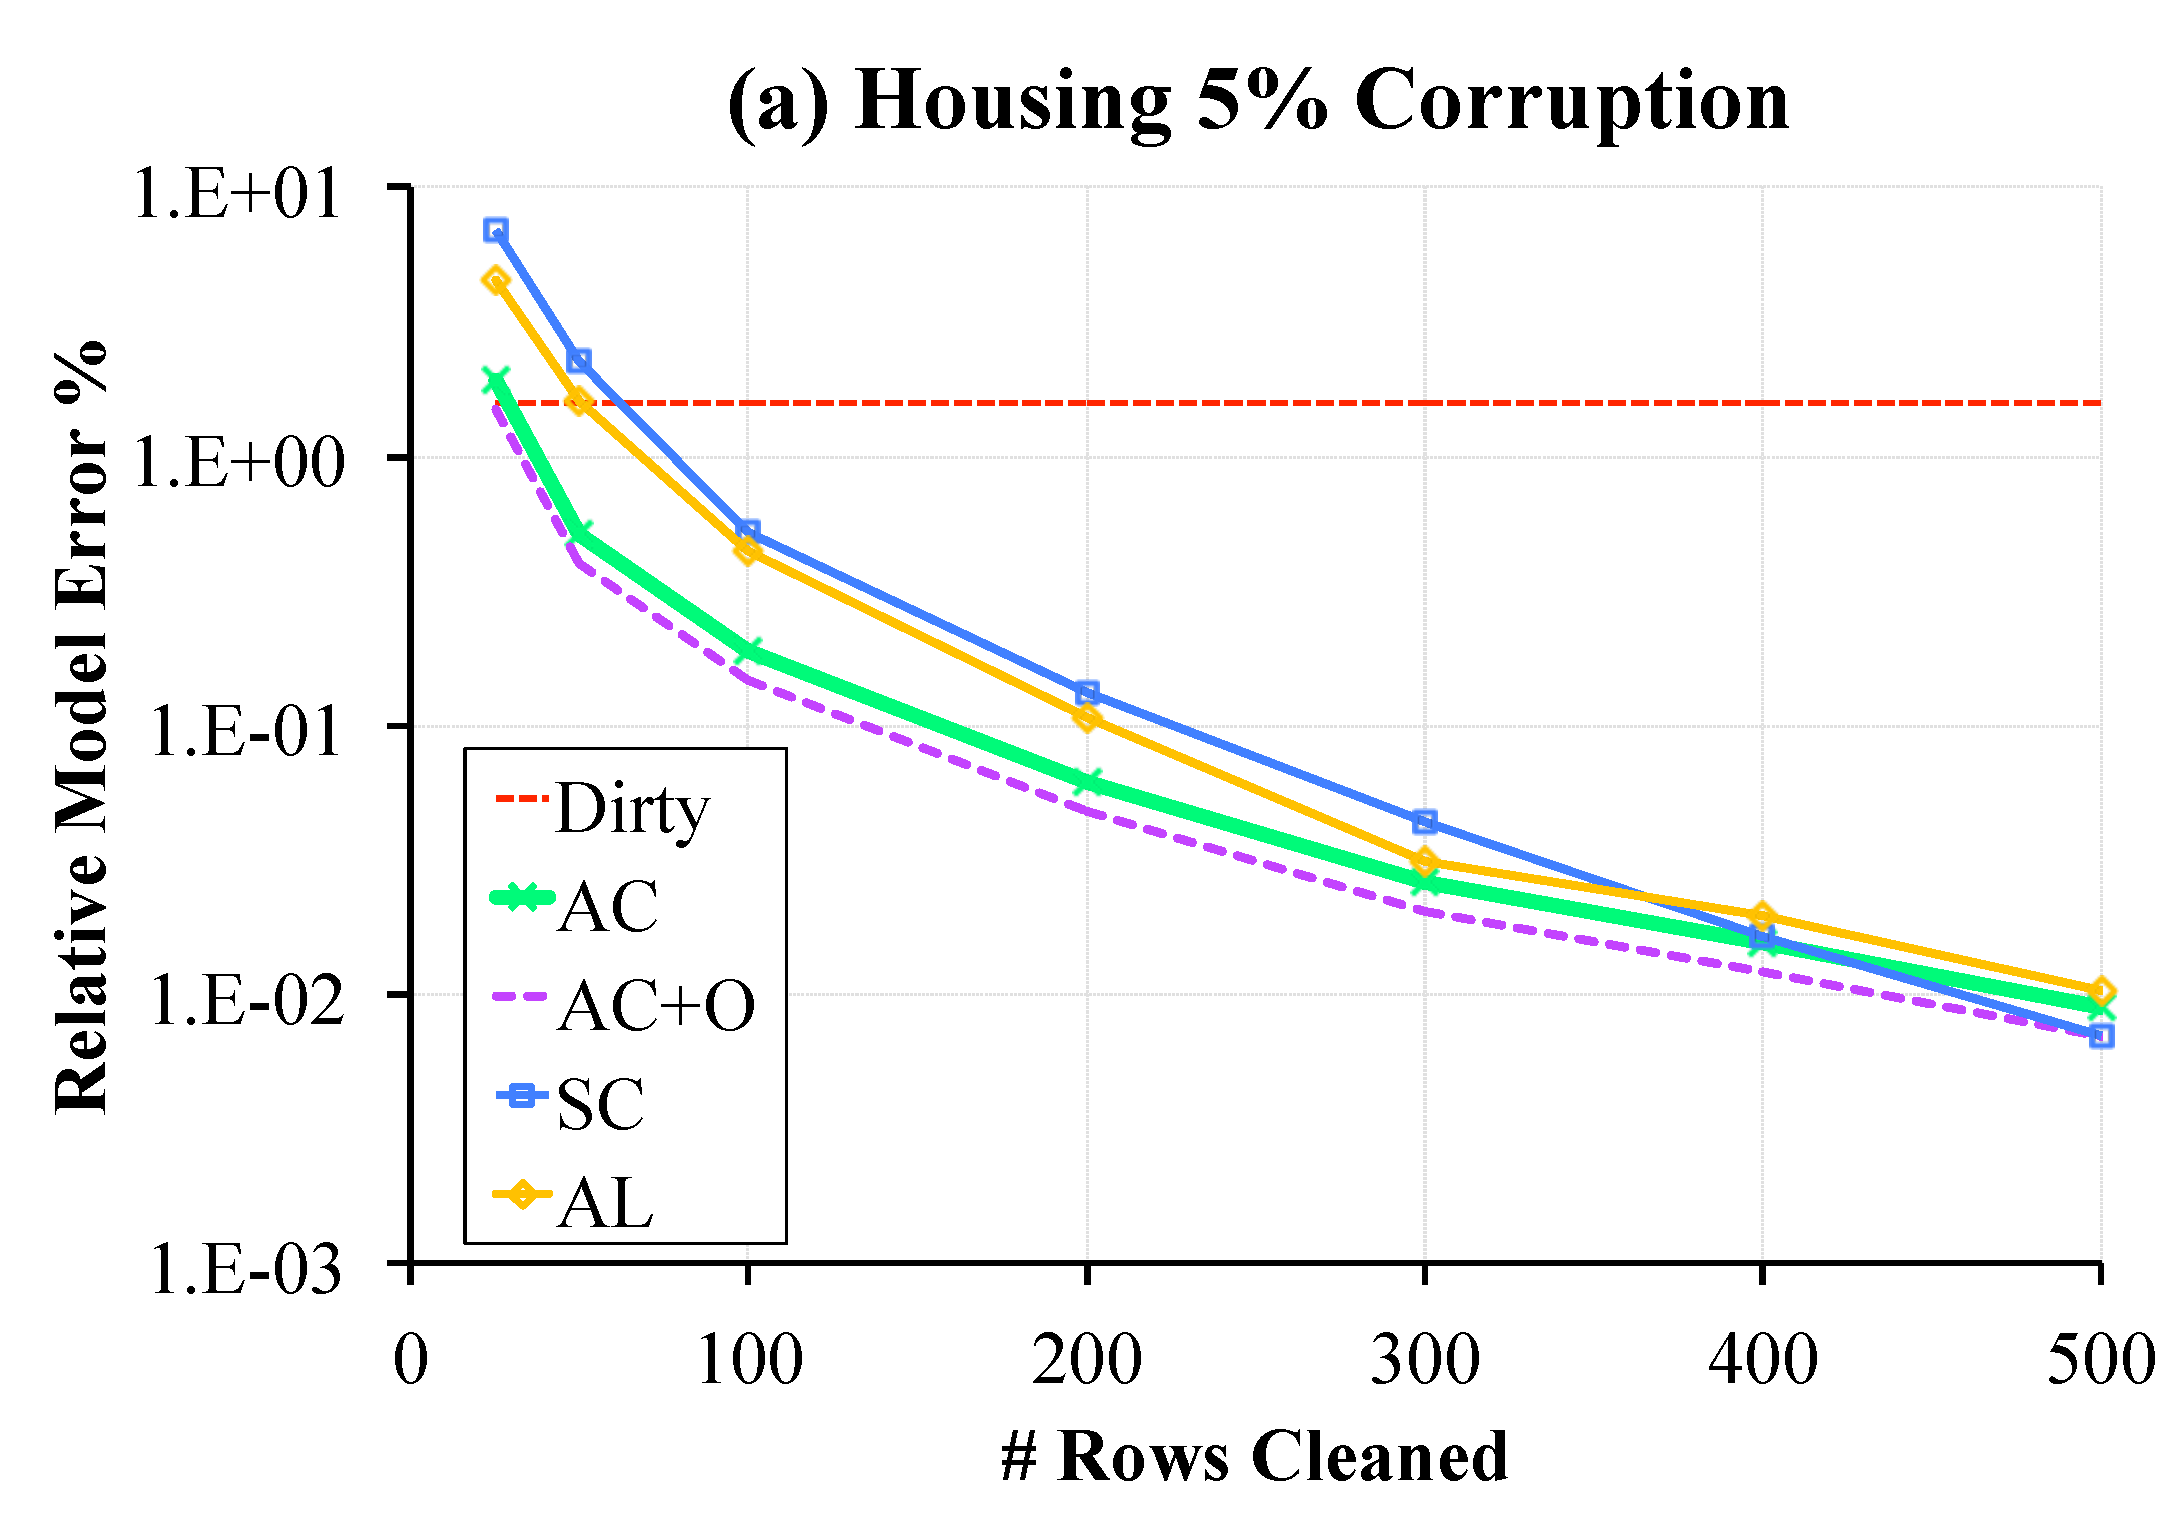
\includegraphics[scale=0.15]{exp/exp3a.pdf}
 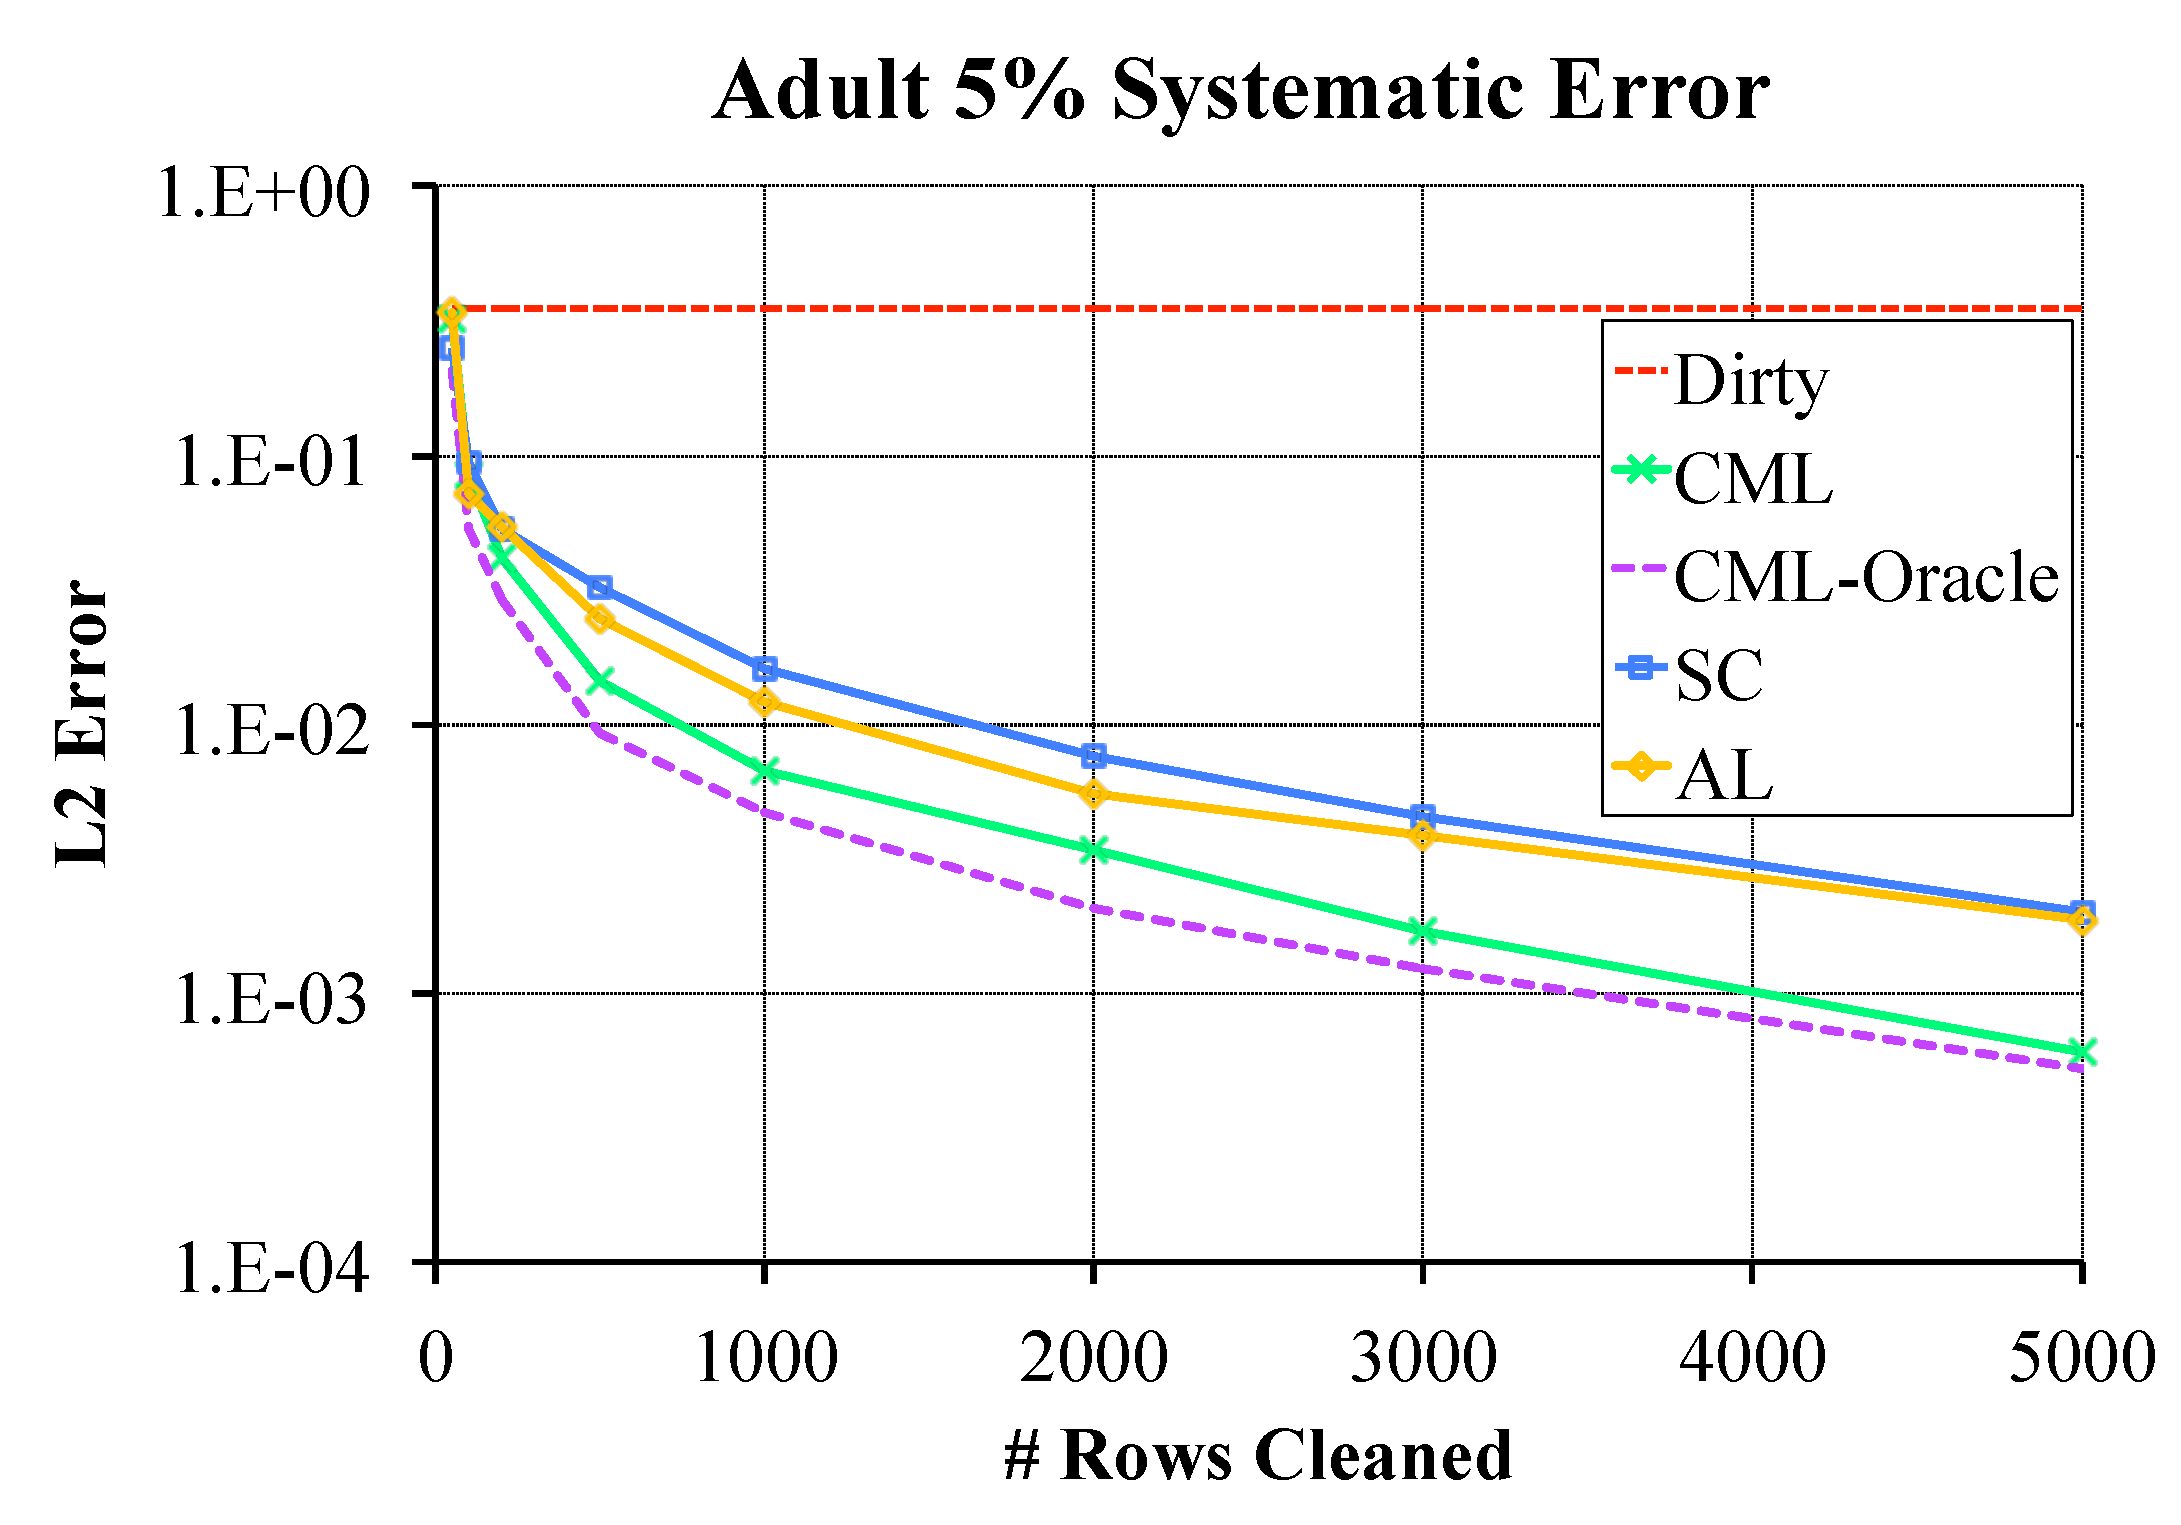
\includegraphics[width=0.49\columnwidth]{exp/exp3b.pdf}
    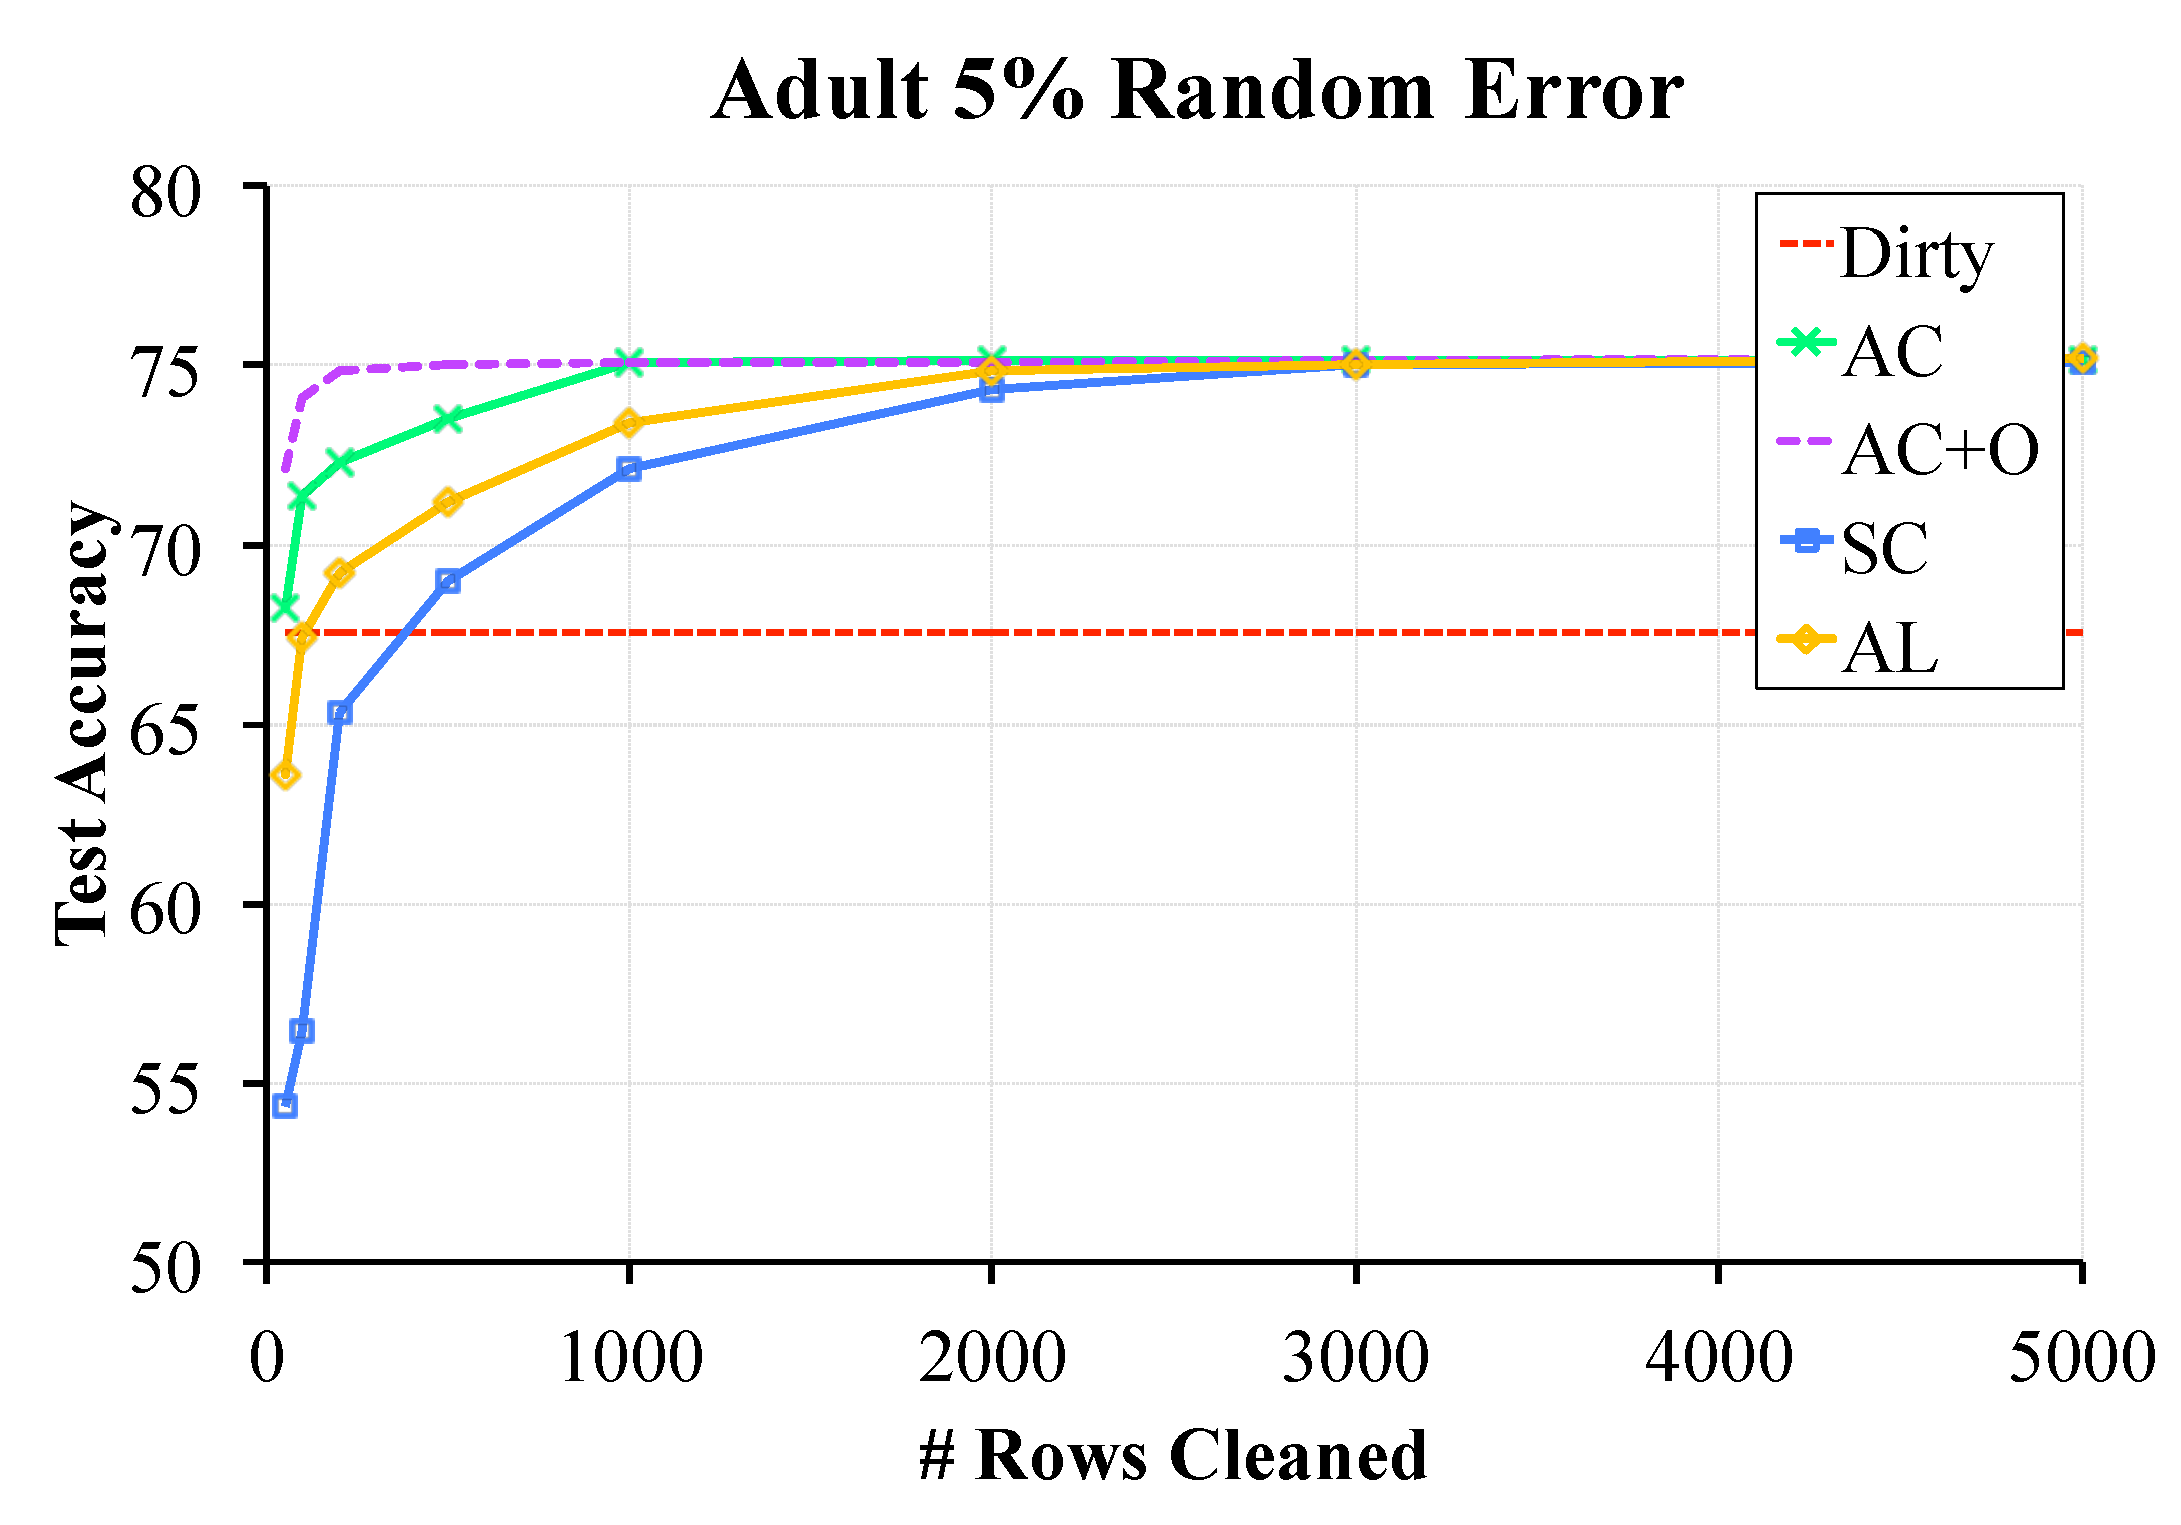
\includegraphics[width=0.49\columnwidth]{exp/exp3bb.pdf}
  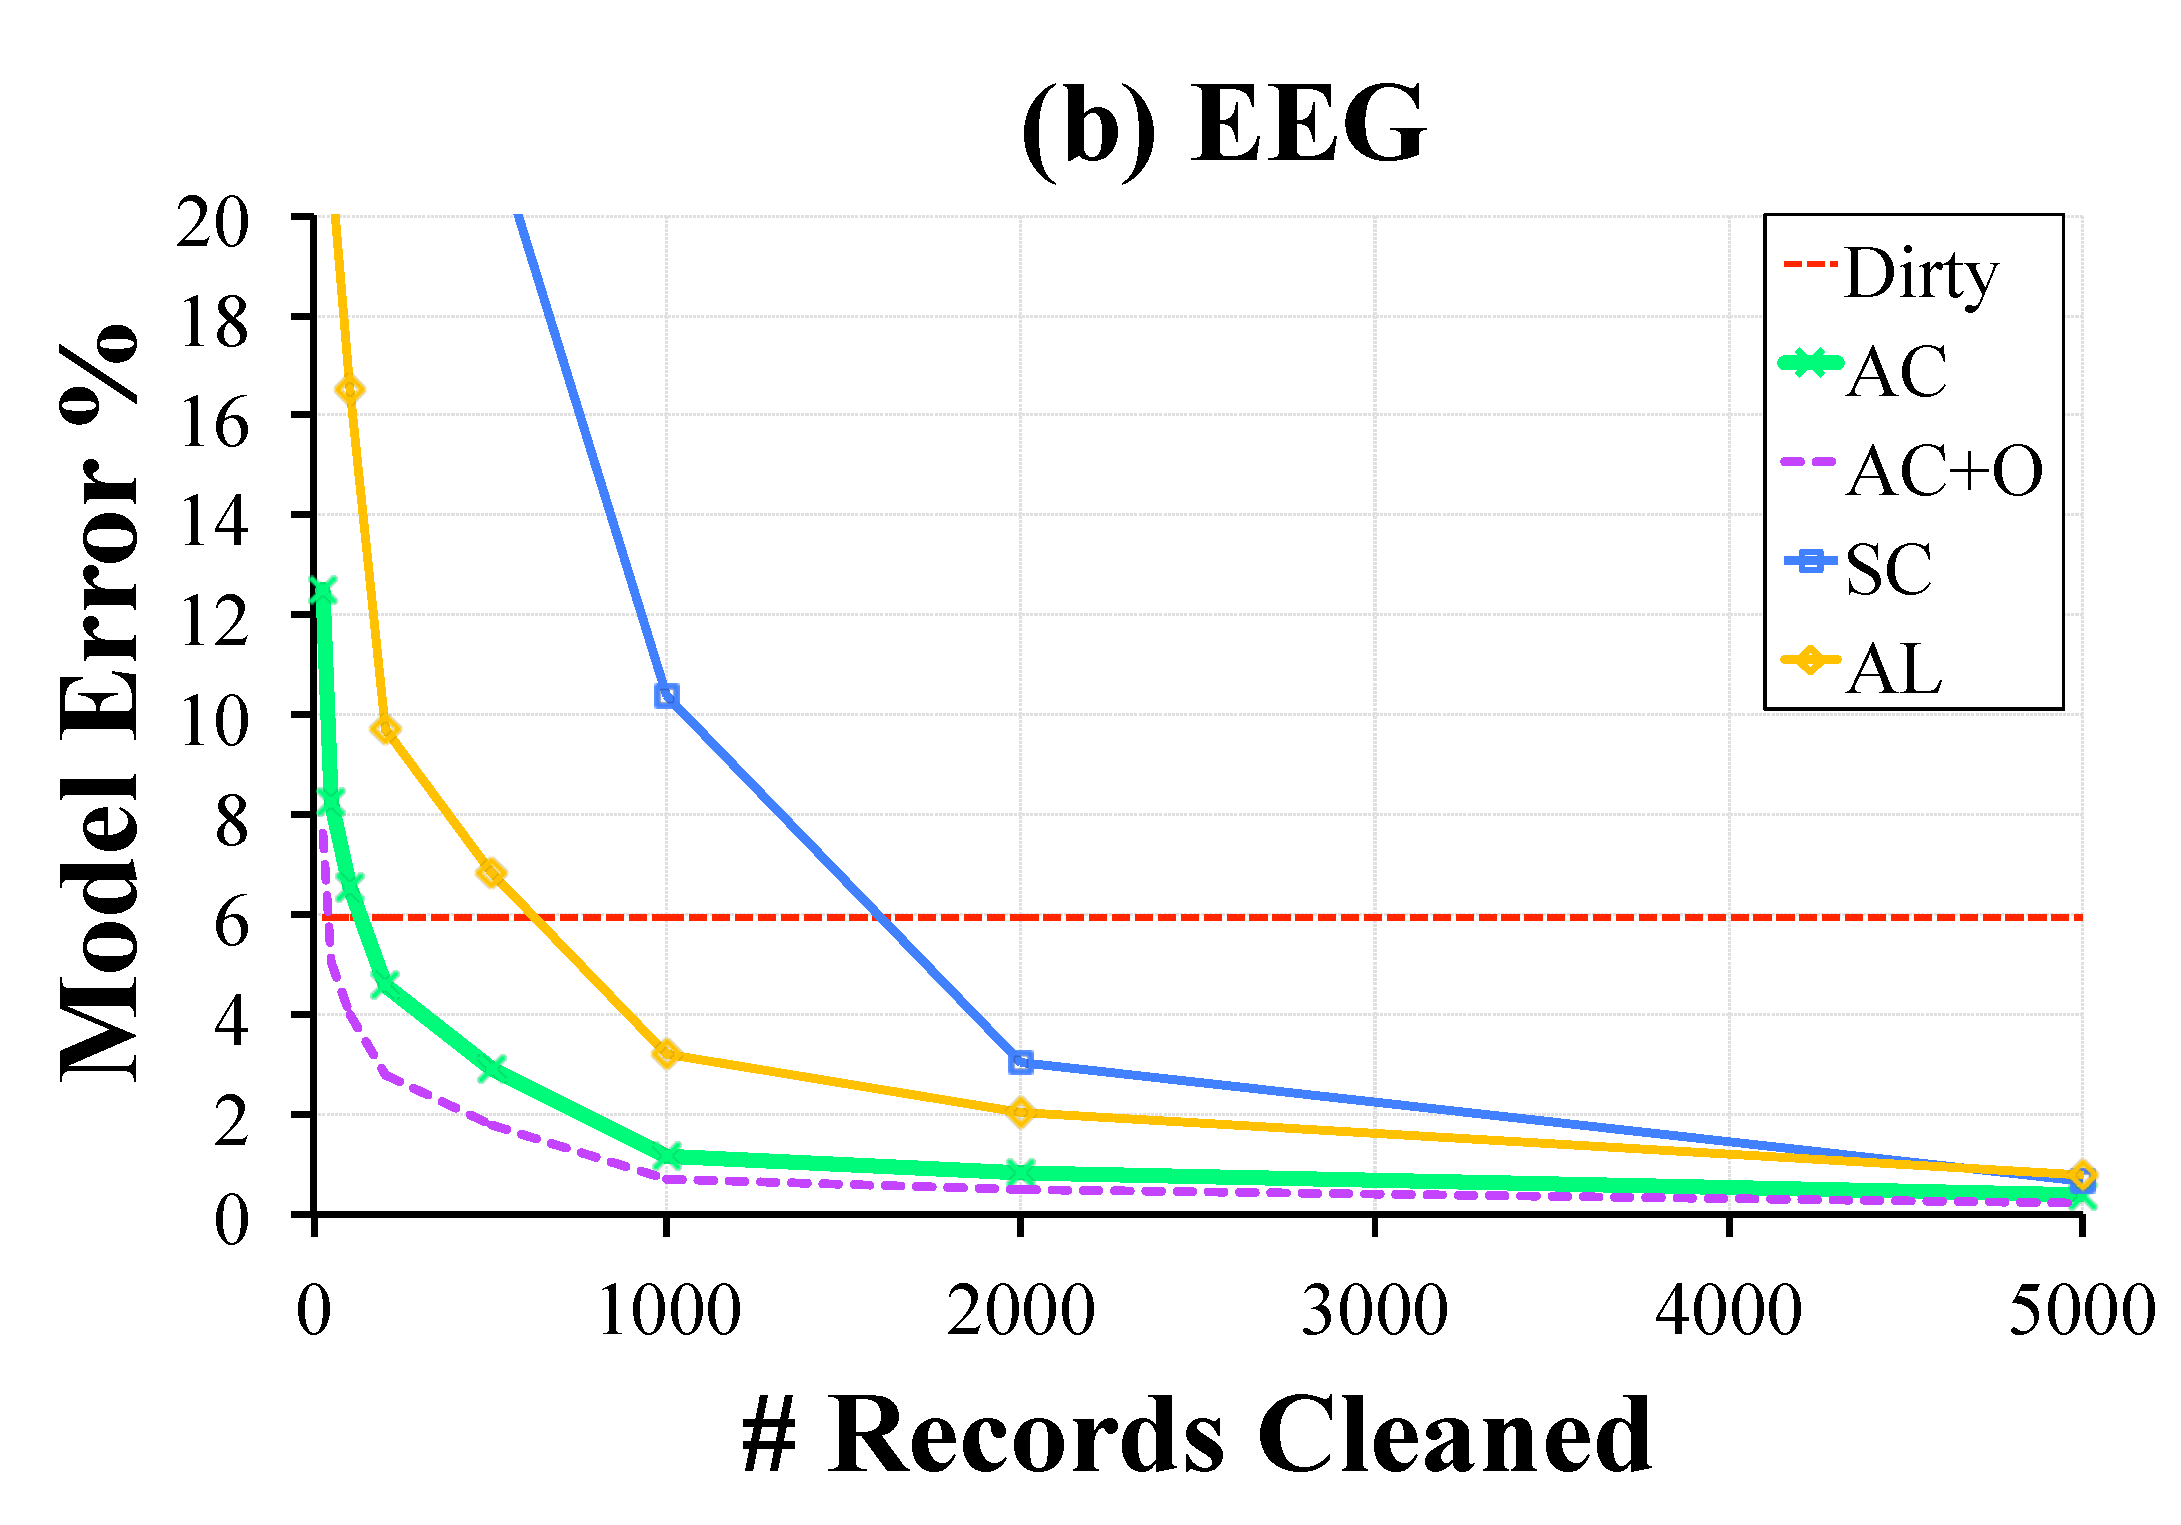
\includegraphics[width=0.49\columnwidth]{exp/exp3c.pdf}
  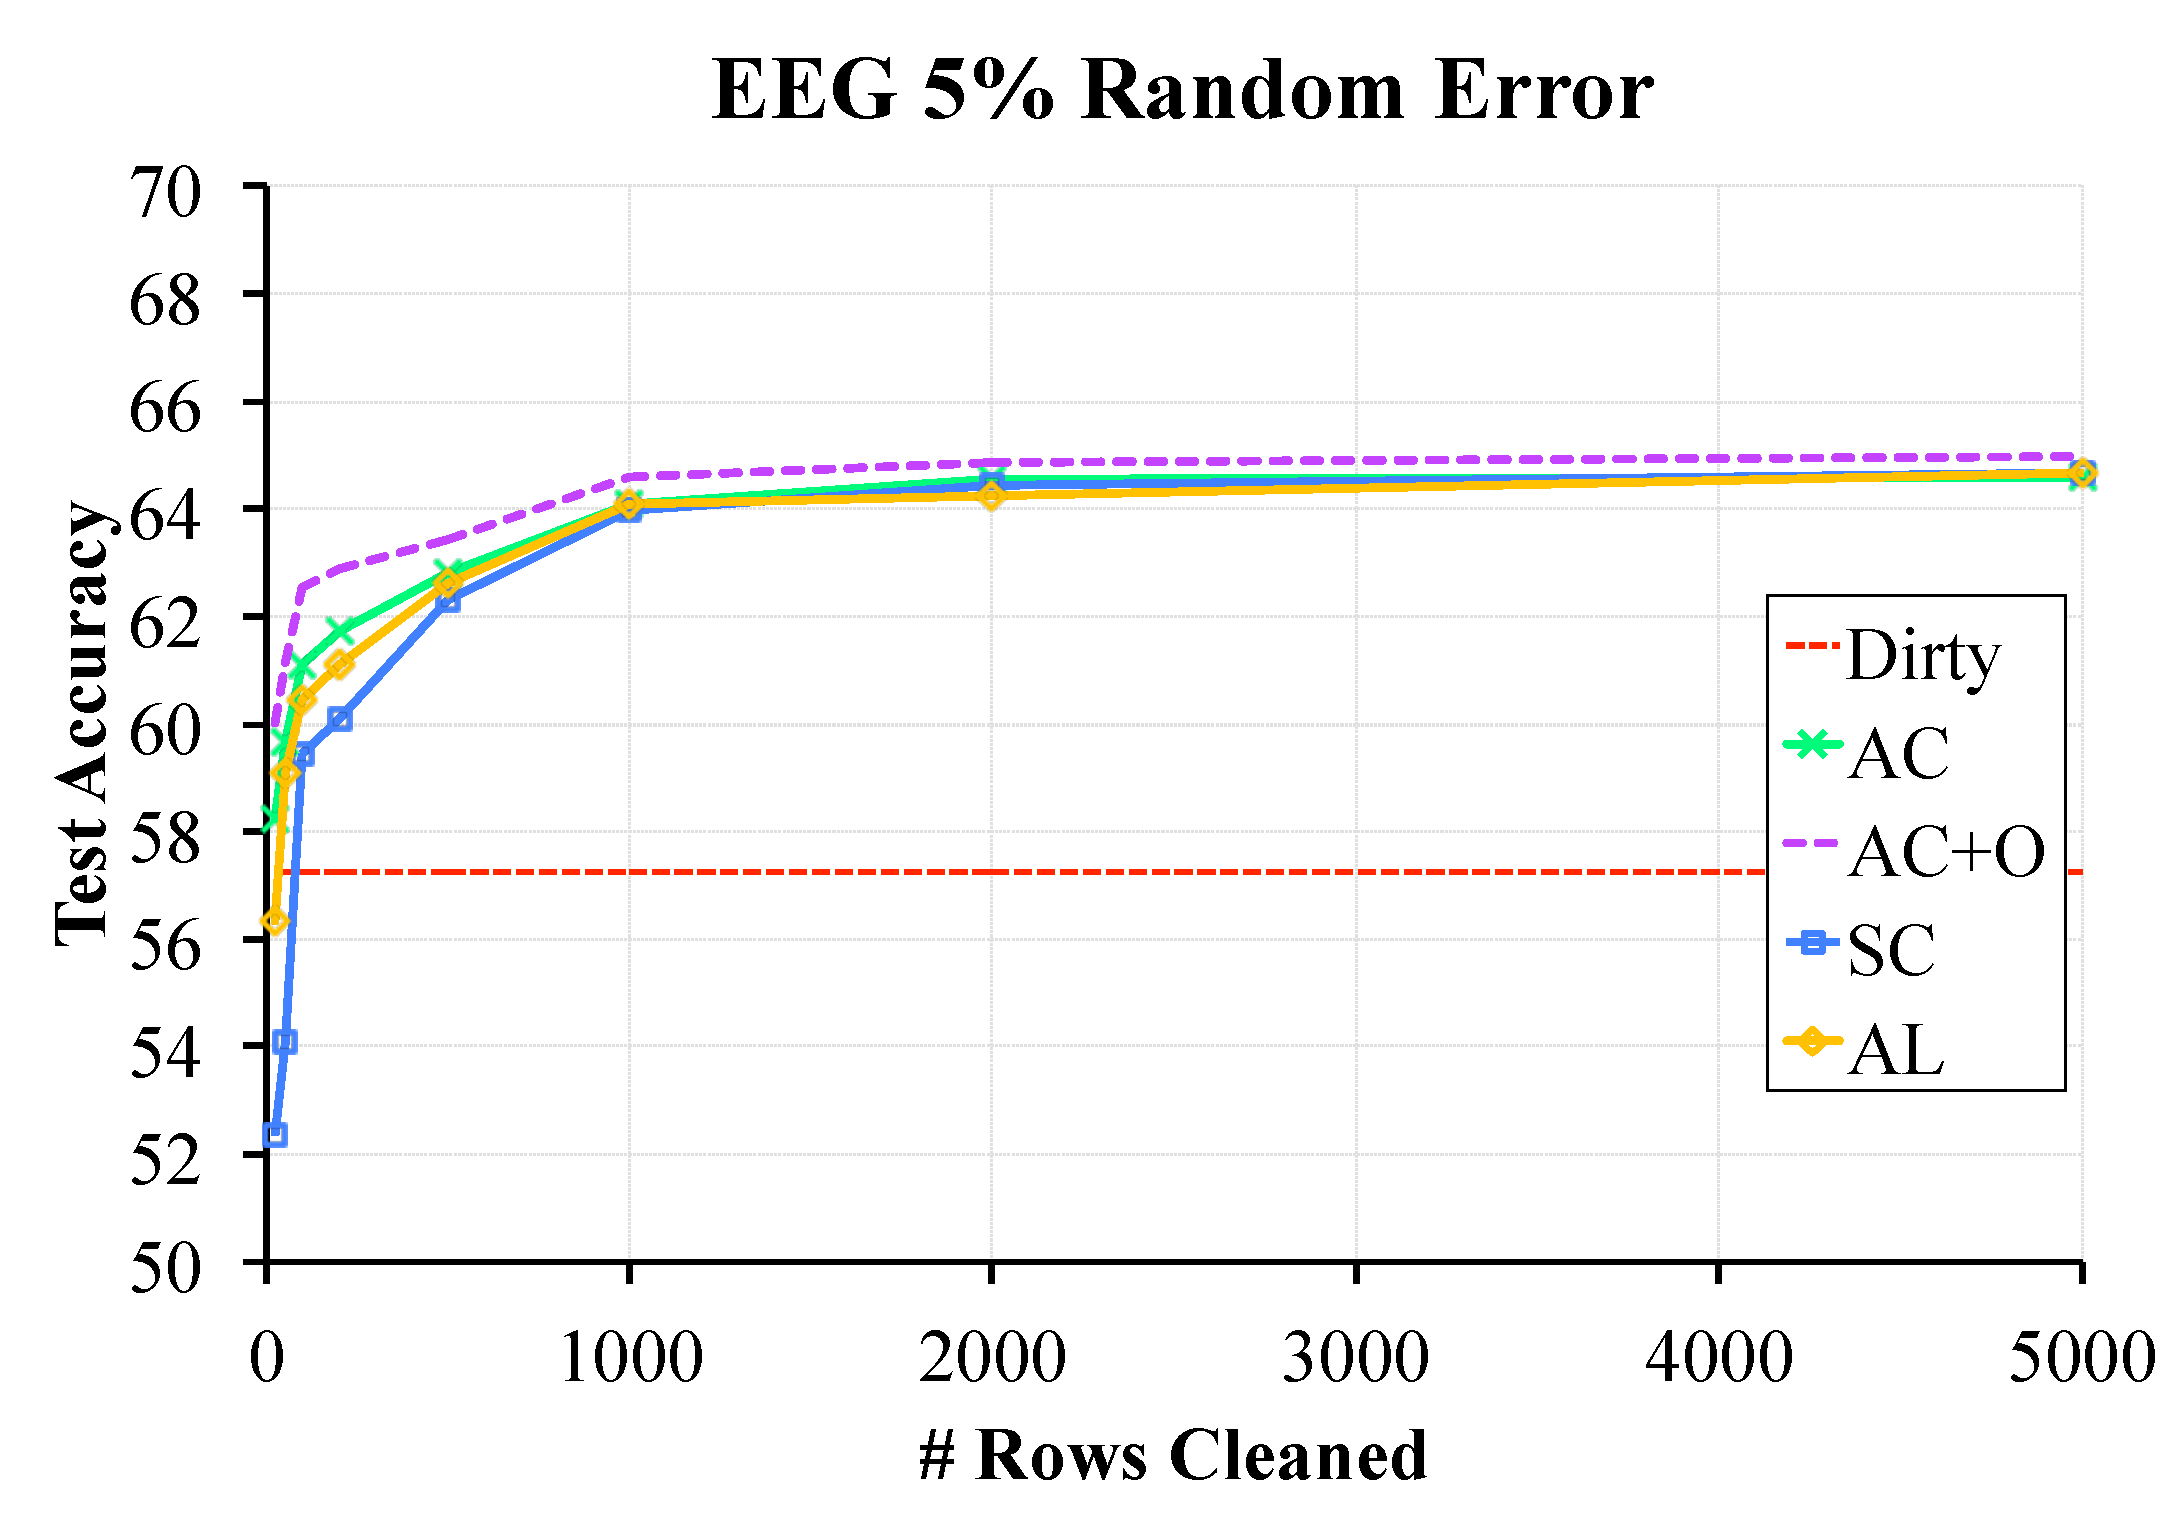
\includegraphics[width=0.49\columnwidth]{exp/exp3cc.pdf}
 \caption{\sys converges with a smaller sample size to the true result in comparison to Active Learning and SampleClean. We show the relative model error as a function of the number of examples cleaned. \label{prio-perf}}
\end{figure}

\subsubsection{Source of Improvements}
Now, we try to understand the source of our improvements w.r.t Active Learning and SampleClean.
We pick a single point on the curves shown in Figure \ref{prio-perf} that corresponds to 500 records cleaned and compare the performance of \sys with and without various optimizations.
This is a vertical slice of the plots in the previous experiments.

We denote \sys without detection as (AC-D) (that is at each iteration we sample from the entire dirty data) and \sys without detection and importance sampling as (AC-D-I).
In Figure \ref{opts}, we plot the relative error of the alternatives and \sys with and without the optimizations.
Detection significantly improves our results in all of the datasets, and accounts for a substantial part of the improvements over Active Learning.
However, when we remove detection we still see some improvements since our importance sampling relies on error impact estimates.
Not surprisingly, when we remove both these optimizations, \sys is slightly worse (but still comparable to) than Active Learning.

\vspace{0.25em}

\noindent \emph{Summary: Both a priori detection and non-uniform sampling significantly contribute to the gains over Active Learning.}

\begin{figure}[ht!]
\centering
 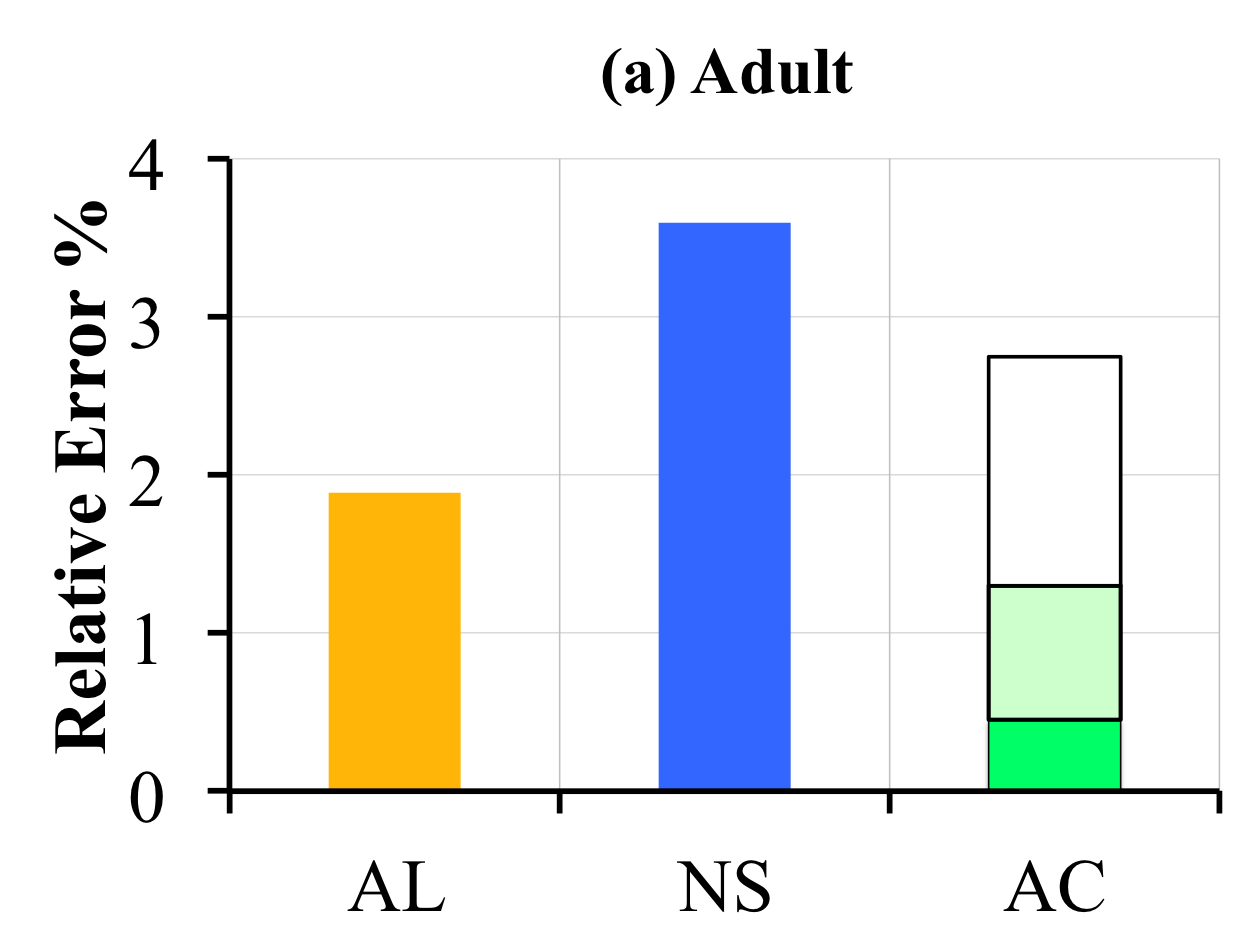
\includegraphics[width=0.49\columnwidth]{exp/exp8a.png}
 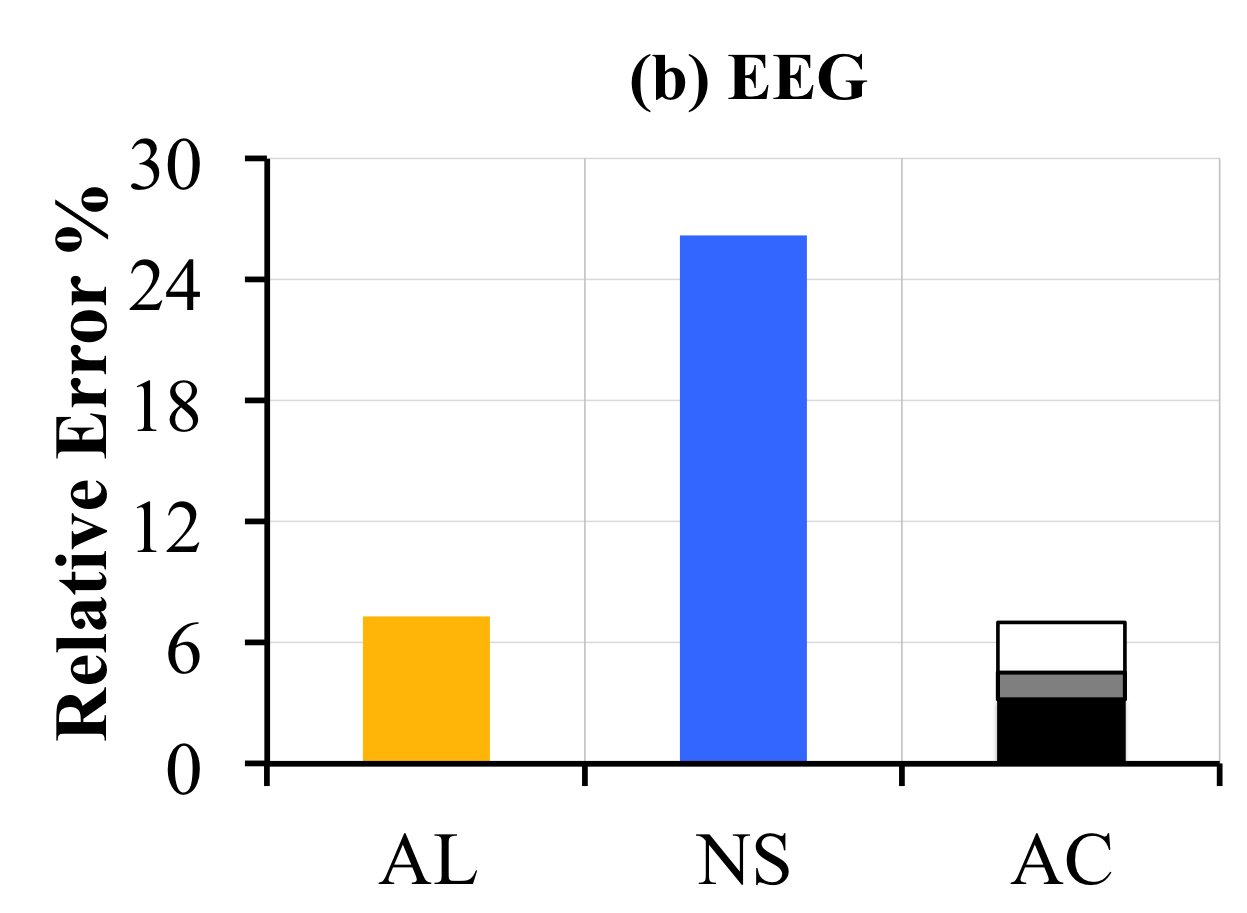
\includegraphics[width=0.49\columnwidth]{exp/exp8b.png}
 \caption{We clean 500 records and plot the relative error of \sys with and without optimizations. -D denotes no detection, and -D-I denotes no detection and no importance sampling. Both optimization significantly help \sys outperform SampleClean and Active Learning. \label{opts}}
\end{figure}

\iffalse
We evalue Active Learning and \sys to better understand this relationship.
In Figure \ref{albias}, we vary the biasing effect of our random corruptions.
That is, we start with zero mean noise and increase the mean value and variance of the noise.
Since Active Learning uses the gradient, if there is zero mean noise, in expectation, the dirty data and clean data are the same.
However, as the bias increases, the fact that Active Learning prioritizes w.r.t to the dirty data matters more and becomes increasingly erroneous w.r.t to \sys.

\begin{figure}[ht!]
\centering
 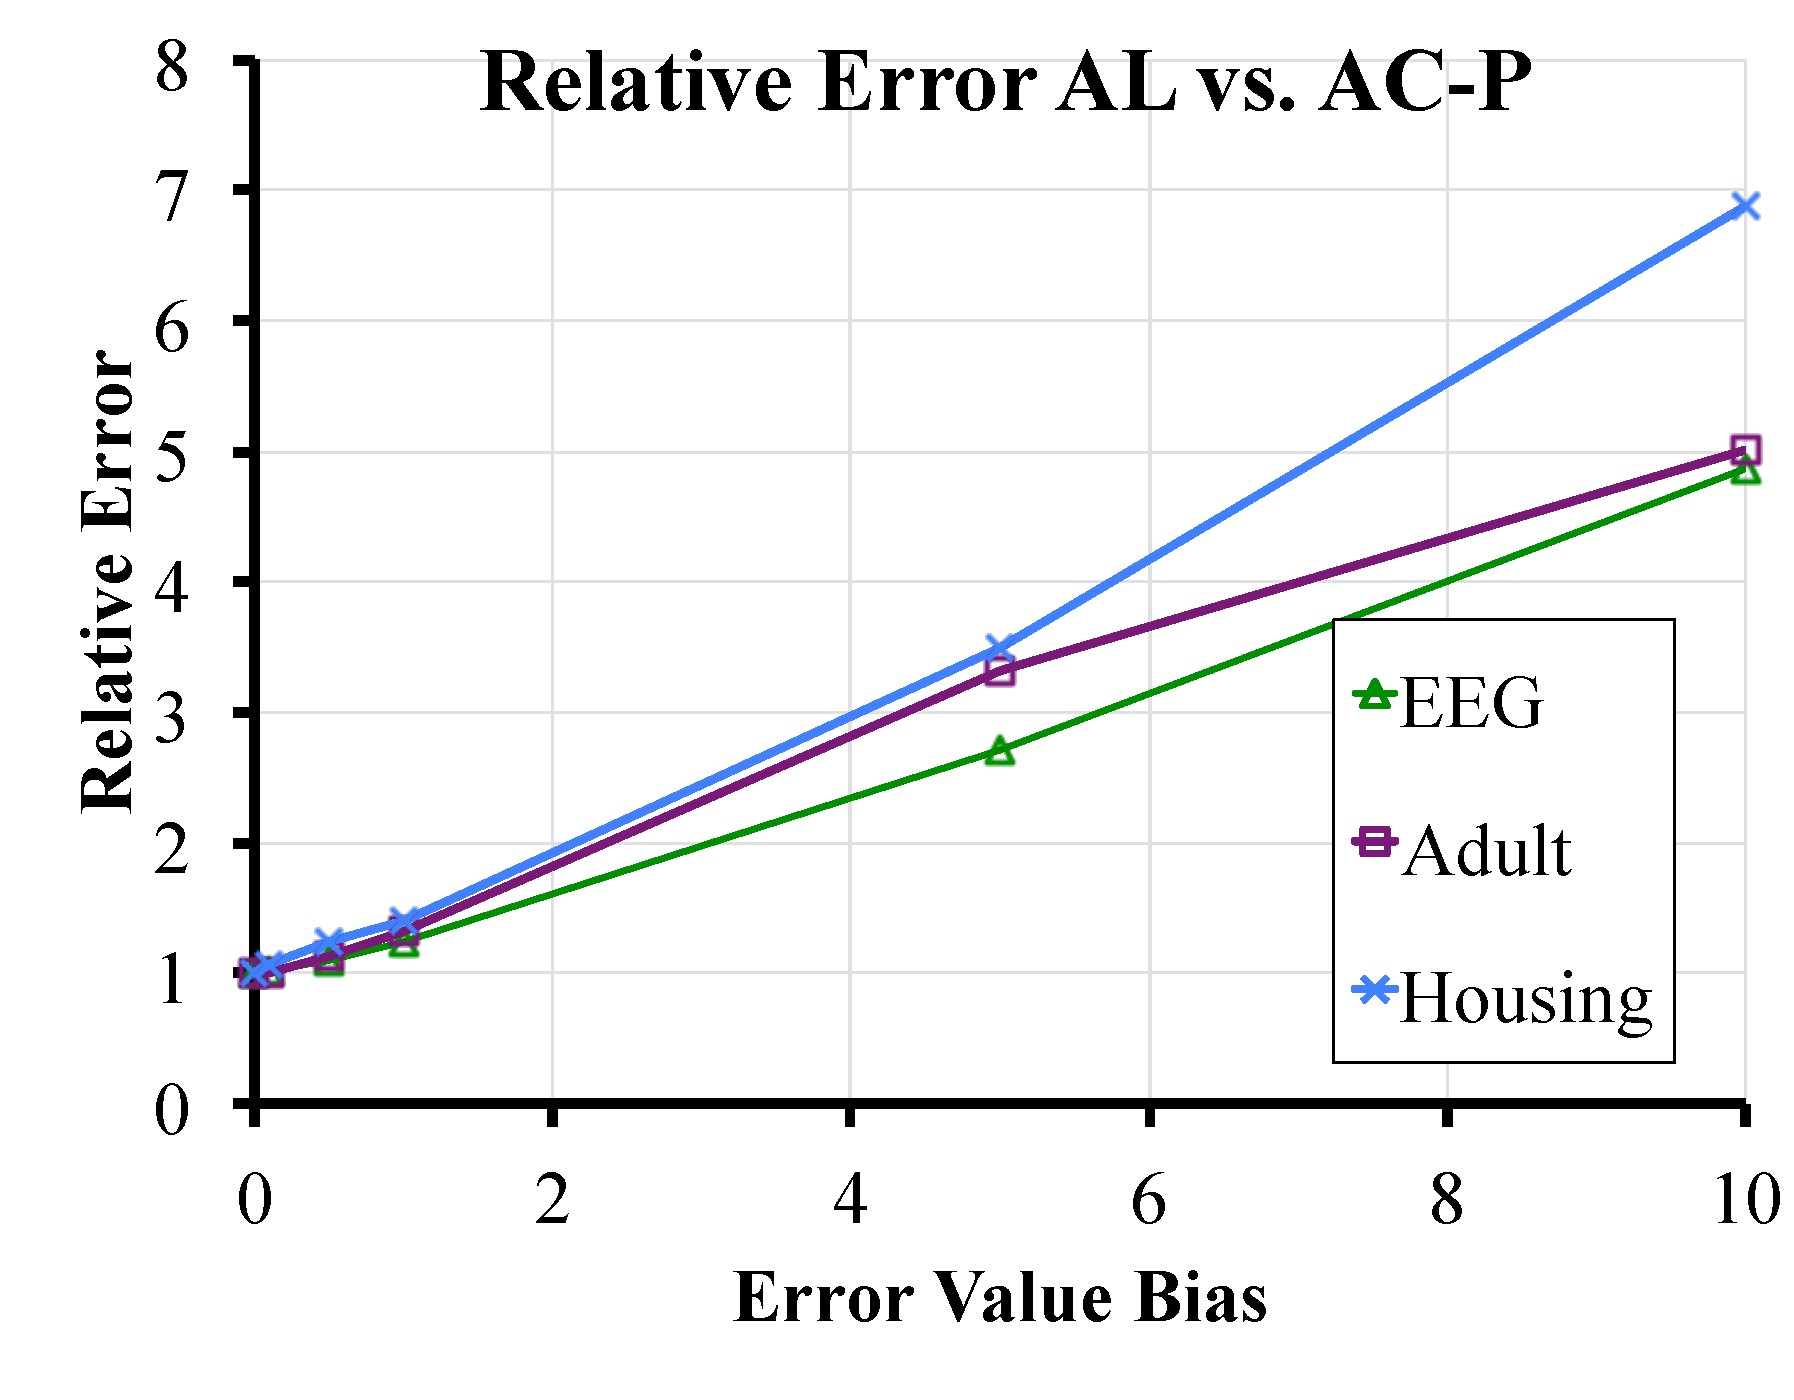
\includegraphics[width=0.6\columnwidth]{exp/exp10.pdf}
 \caption{As we increase the biasing nature of the corruption, Active Learning is increasingly erroneous w.r.t \sys. \label{albias}}
\end{figure}
\fi

\subsubsection{Comparison with Partial Cleaning}
We argue that training a model on partially cleaned is an unreliable methodology lacking the same guarantees as Active Learning or SampleClean even in the simplest of cases.
It is easy to construct errors for which cleaning more data may counter intuitively increase model error.
For thoroughness, we include the tradeoff curves in comparison to \sys for the errors that we generated.
In Figure \ref{pc-perf}, we plot the same curves as the previous experiment comparing \sys, Active Learning, and two partial cleaning algorithms.
First, we randomly sample data, clean, and write-back the cleaned data (denoted as PC).
Next, we randomly sample data from our dirty data detector, clean, and write-back the cleaned data (denoted as PC+D).
We find that for these errors PC and PC+D give reasonable results (not always guaranteed) but \sys converges faster.
This is because \sys tunes the weighting when averaging dirty and clean data into the gradient.

\begin{figure}[ht!]
\centering
 %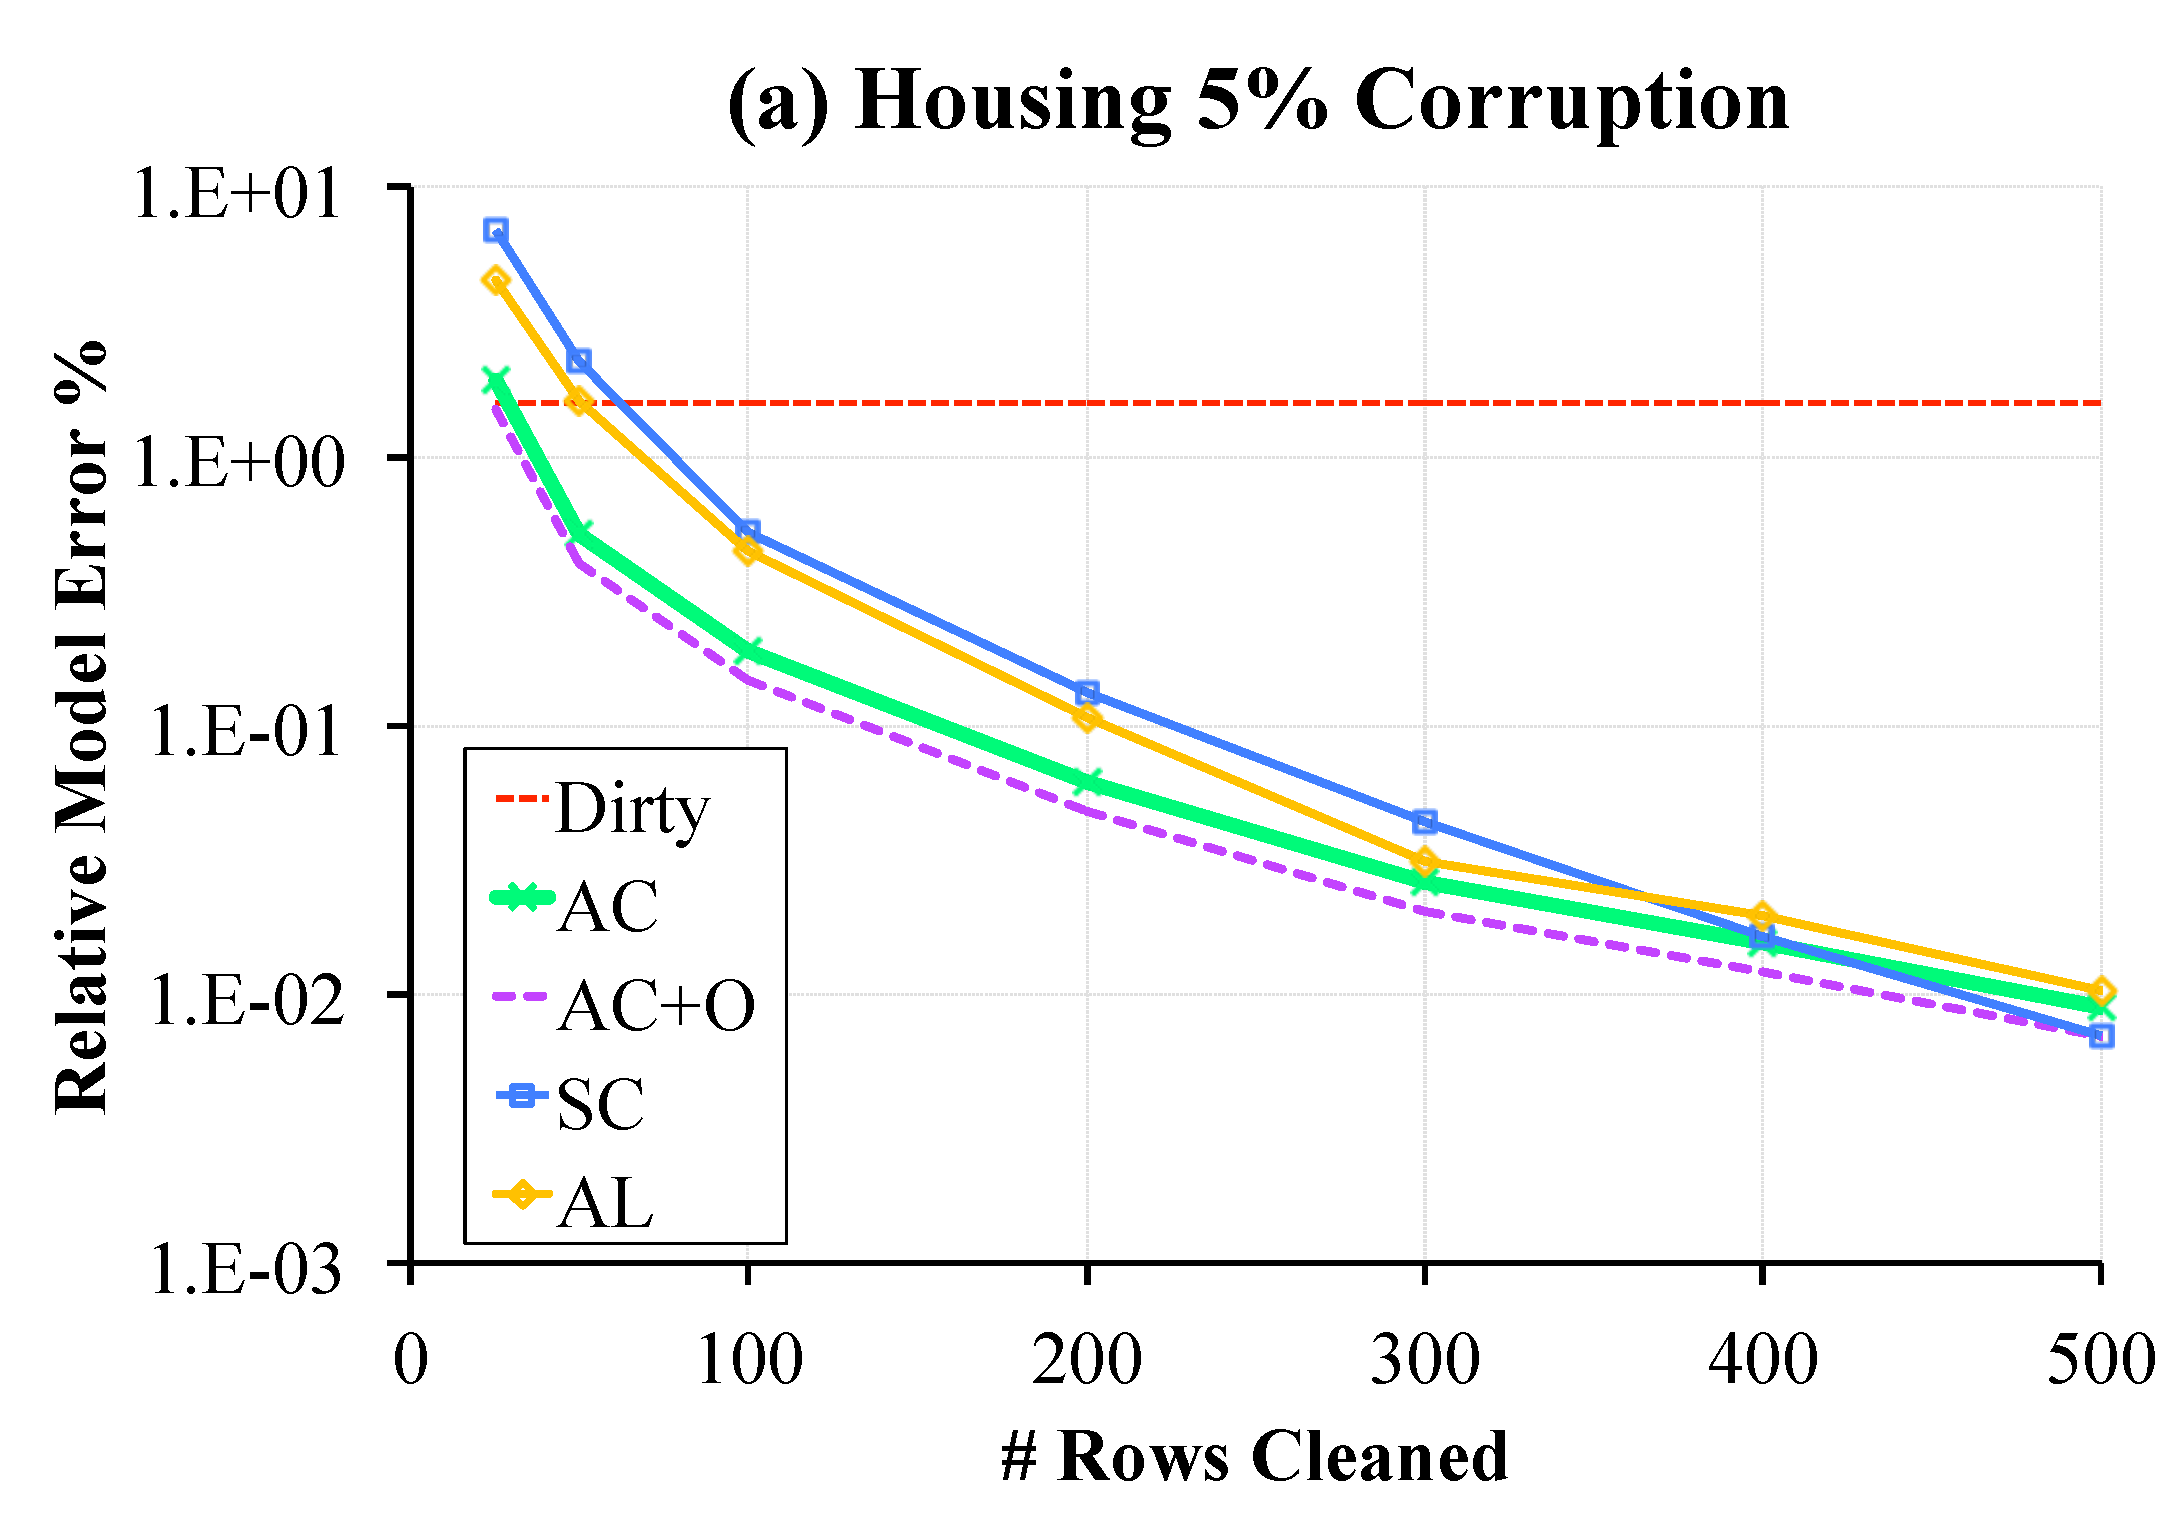
\includegraphics[scale=0.15]{exp/exp3a.pdf}
 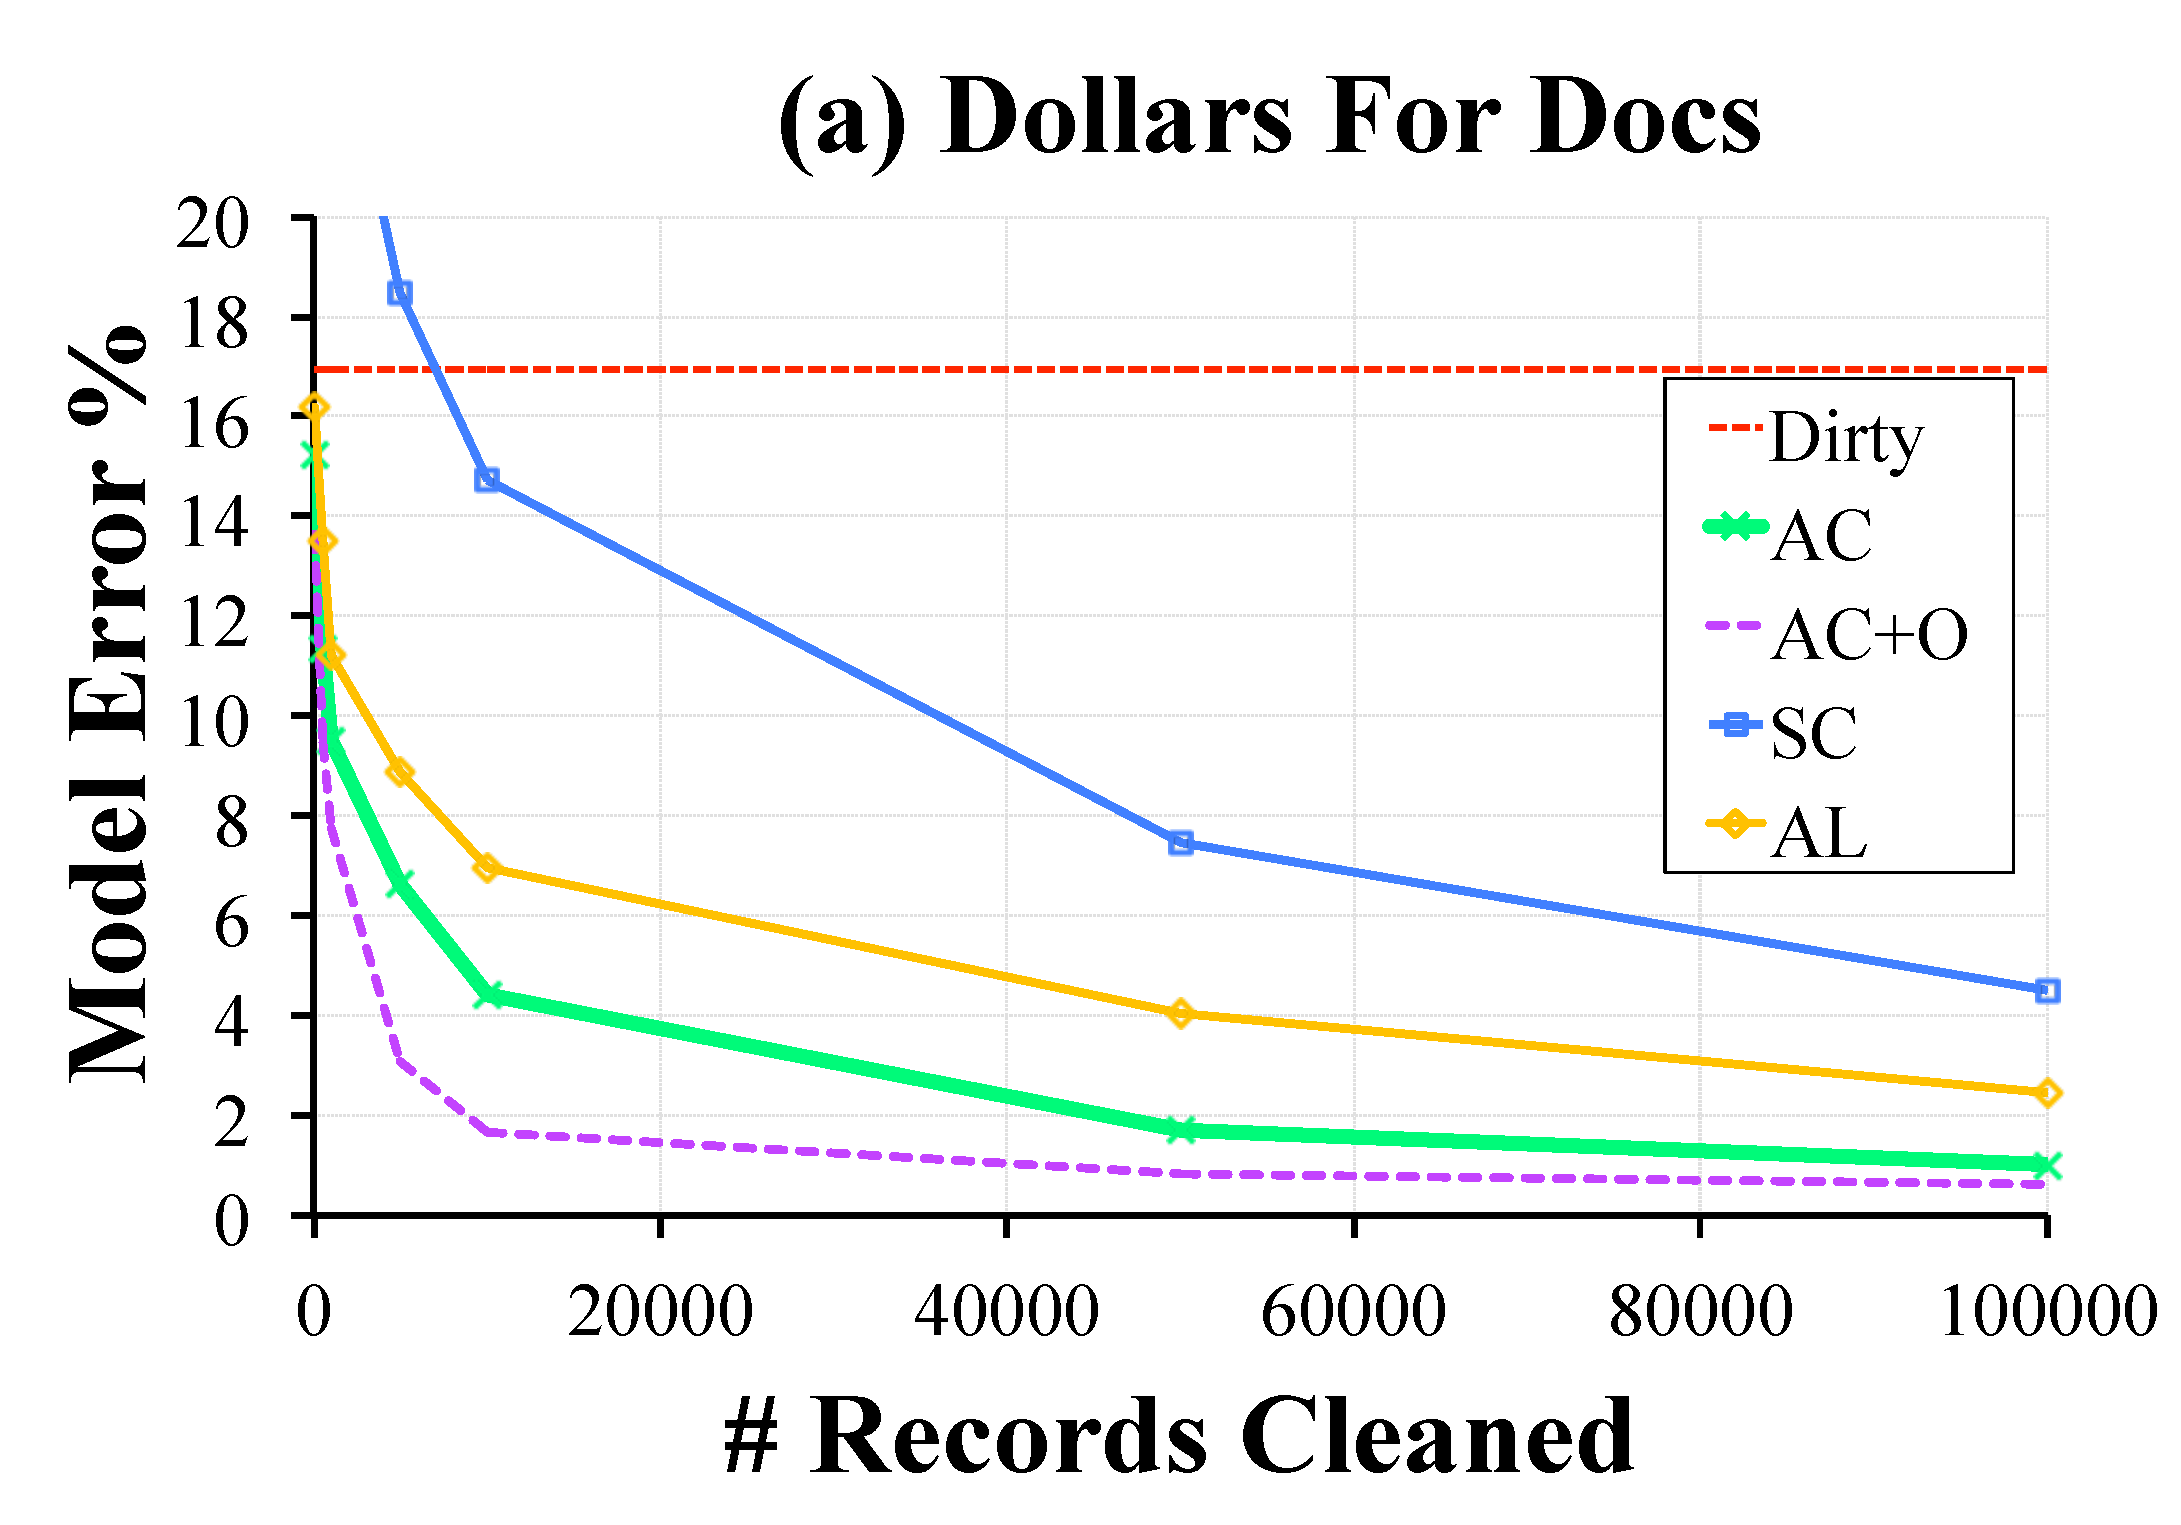
\includegraphics[width=0.49\columnwidth]{exp/exp14a.pdf}
    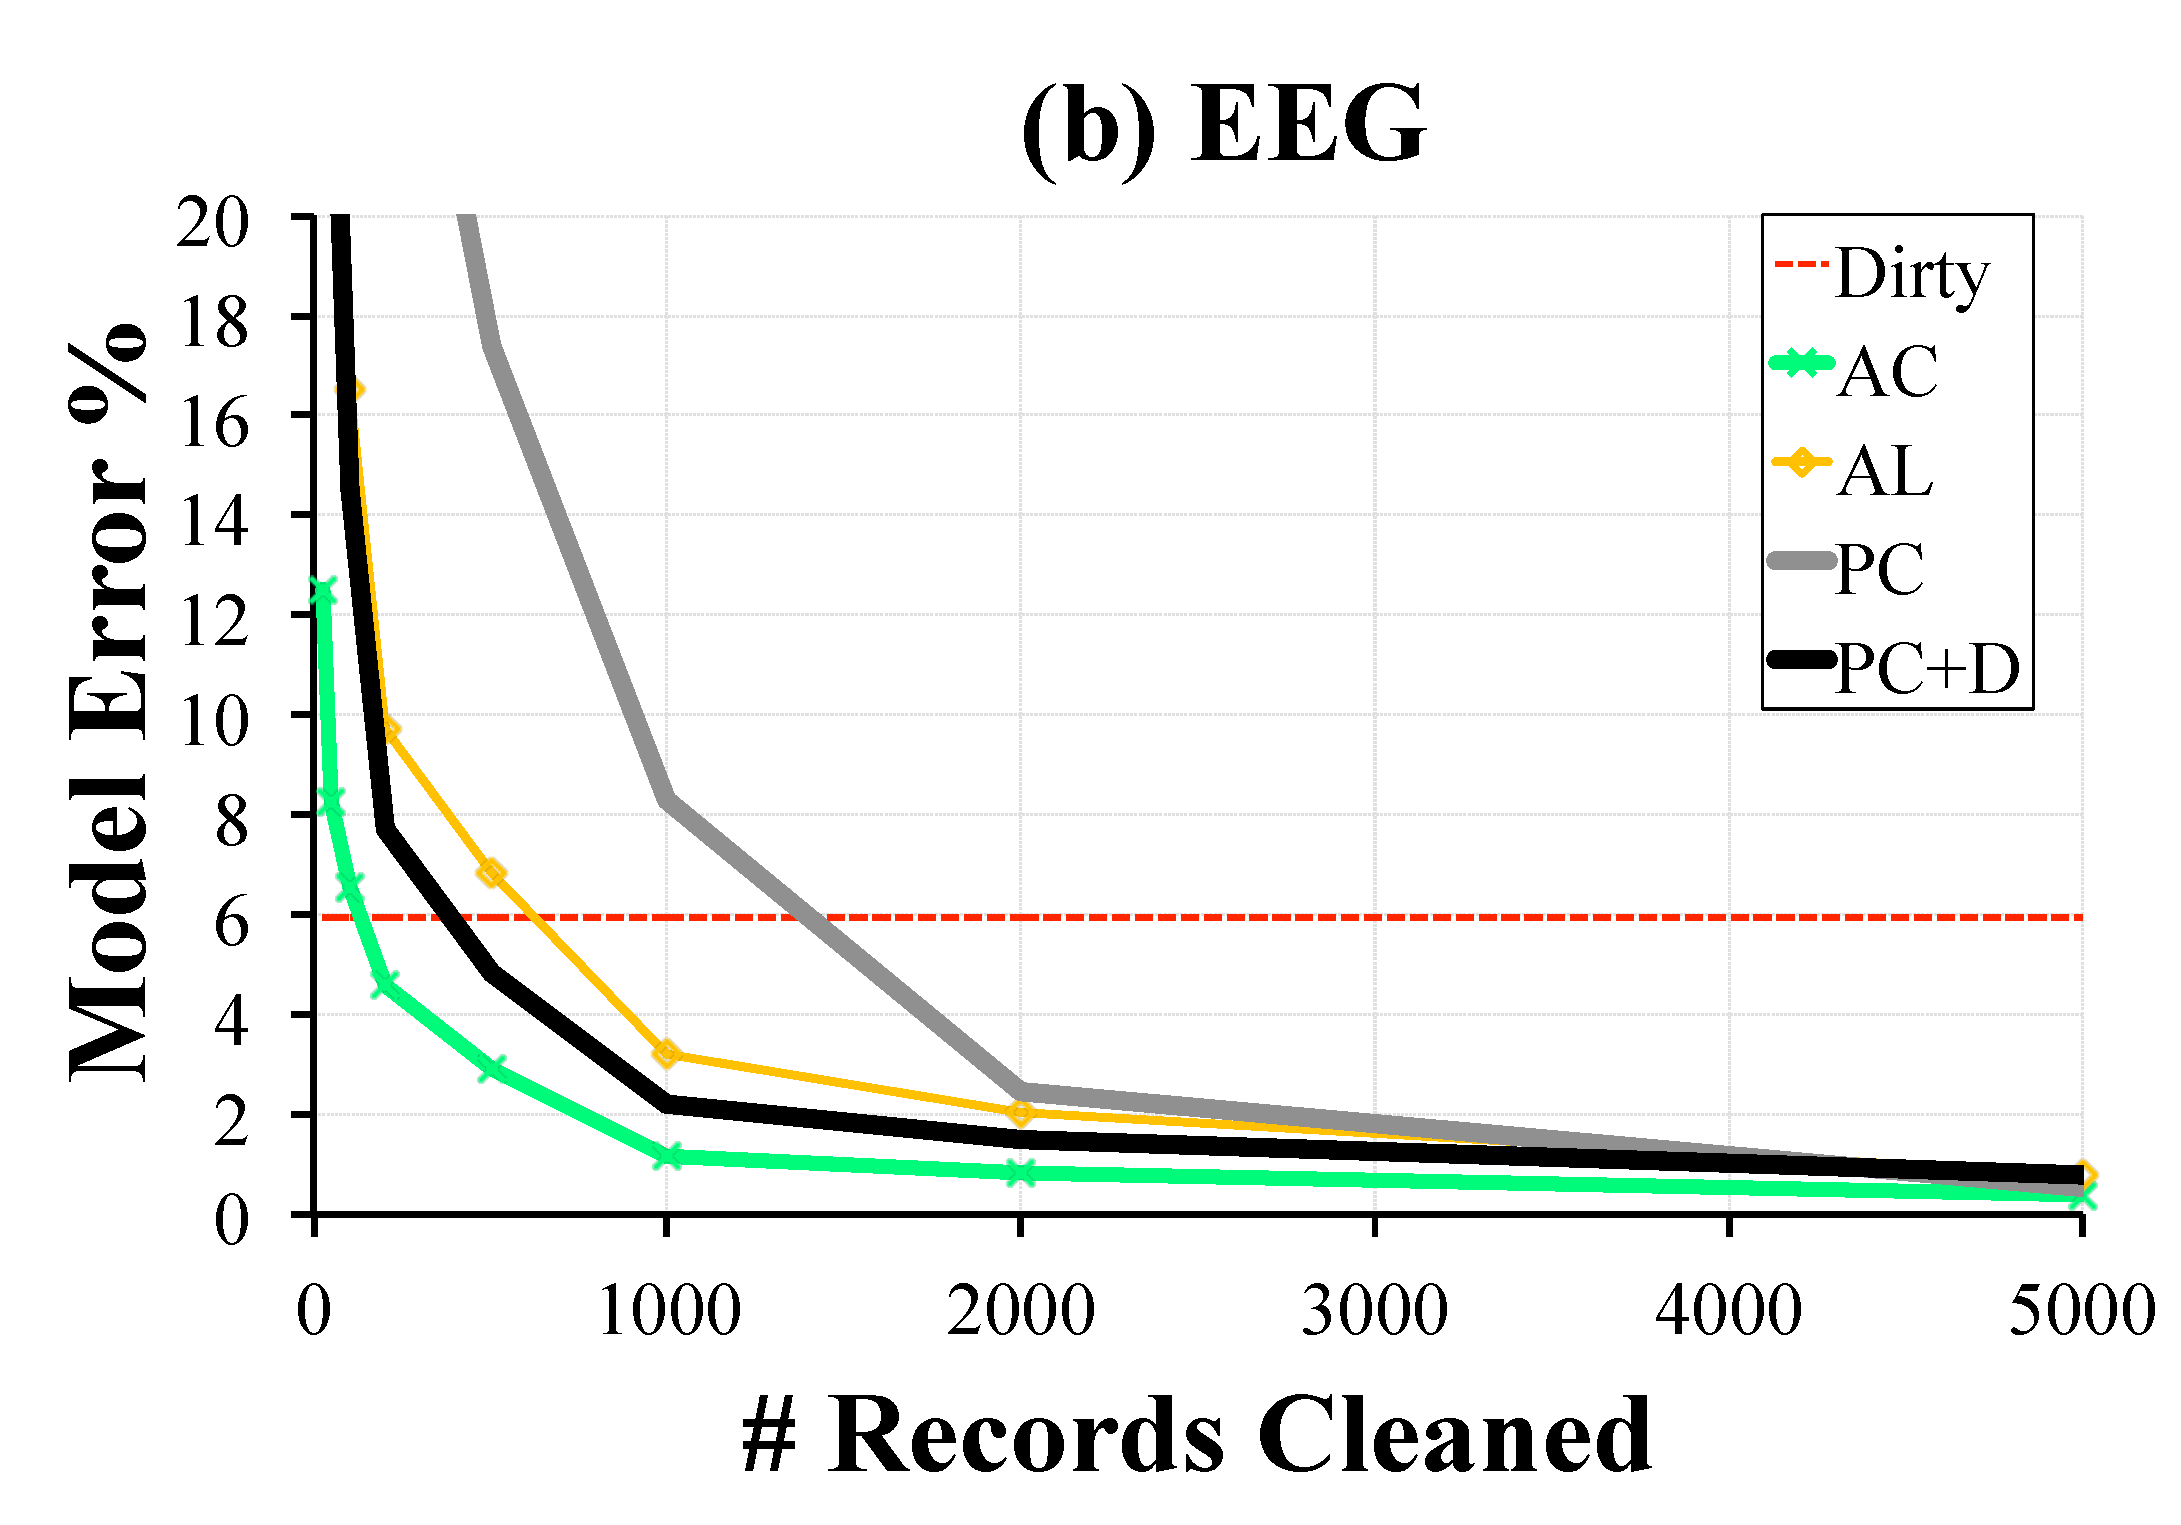
\includegraphics[width=0.49\columnwidth]{exp/exp14b.pdf}
 \caption{\sys converges with a smaller sample size to the true result in comparison to partial cleaning (PC,PC+D). We show the relative model error as a function of the number of examples cleaned. \label{pc-perf}}
\end{figure}

\noindent \emph{Summary: \sys converges faster than partial cleaning since it reweights data based on the fraction that is dirty and clean. Partial cleaning is not guaranteed to give sensible results.}

\subsubsection{Corruption Rate}
Both Active Learning and \sys outperform SampleClean in our experiments.
In our next experiment (Figure \ref{bias}), we try to understand how much of this performance 
is due to the initialization (i.e., SampleClean trains a model from ``scratch").
We vary the systematic corruption rate and plot the number of records cleaned to achieve 1\% relative error for SampleClean and \sys.
SampleClean does not use the dirty data and thus is not dependent on this rate.
We find that SampleClean outperforms \sys only when corruptions are very severe (45\% in Adult and nearly 60\% in EEG). 

\vspace{0.25em}

\noindent \emph{Summary: SampleClean is beneficial in comparison to \sys when corruption rats exceed 45\% in our experiments.}

\begin{figure}[ht!]
\centering
 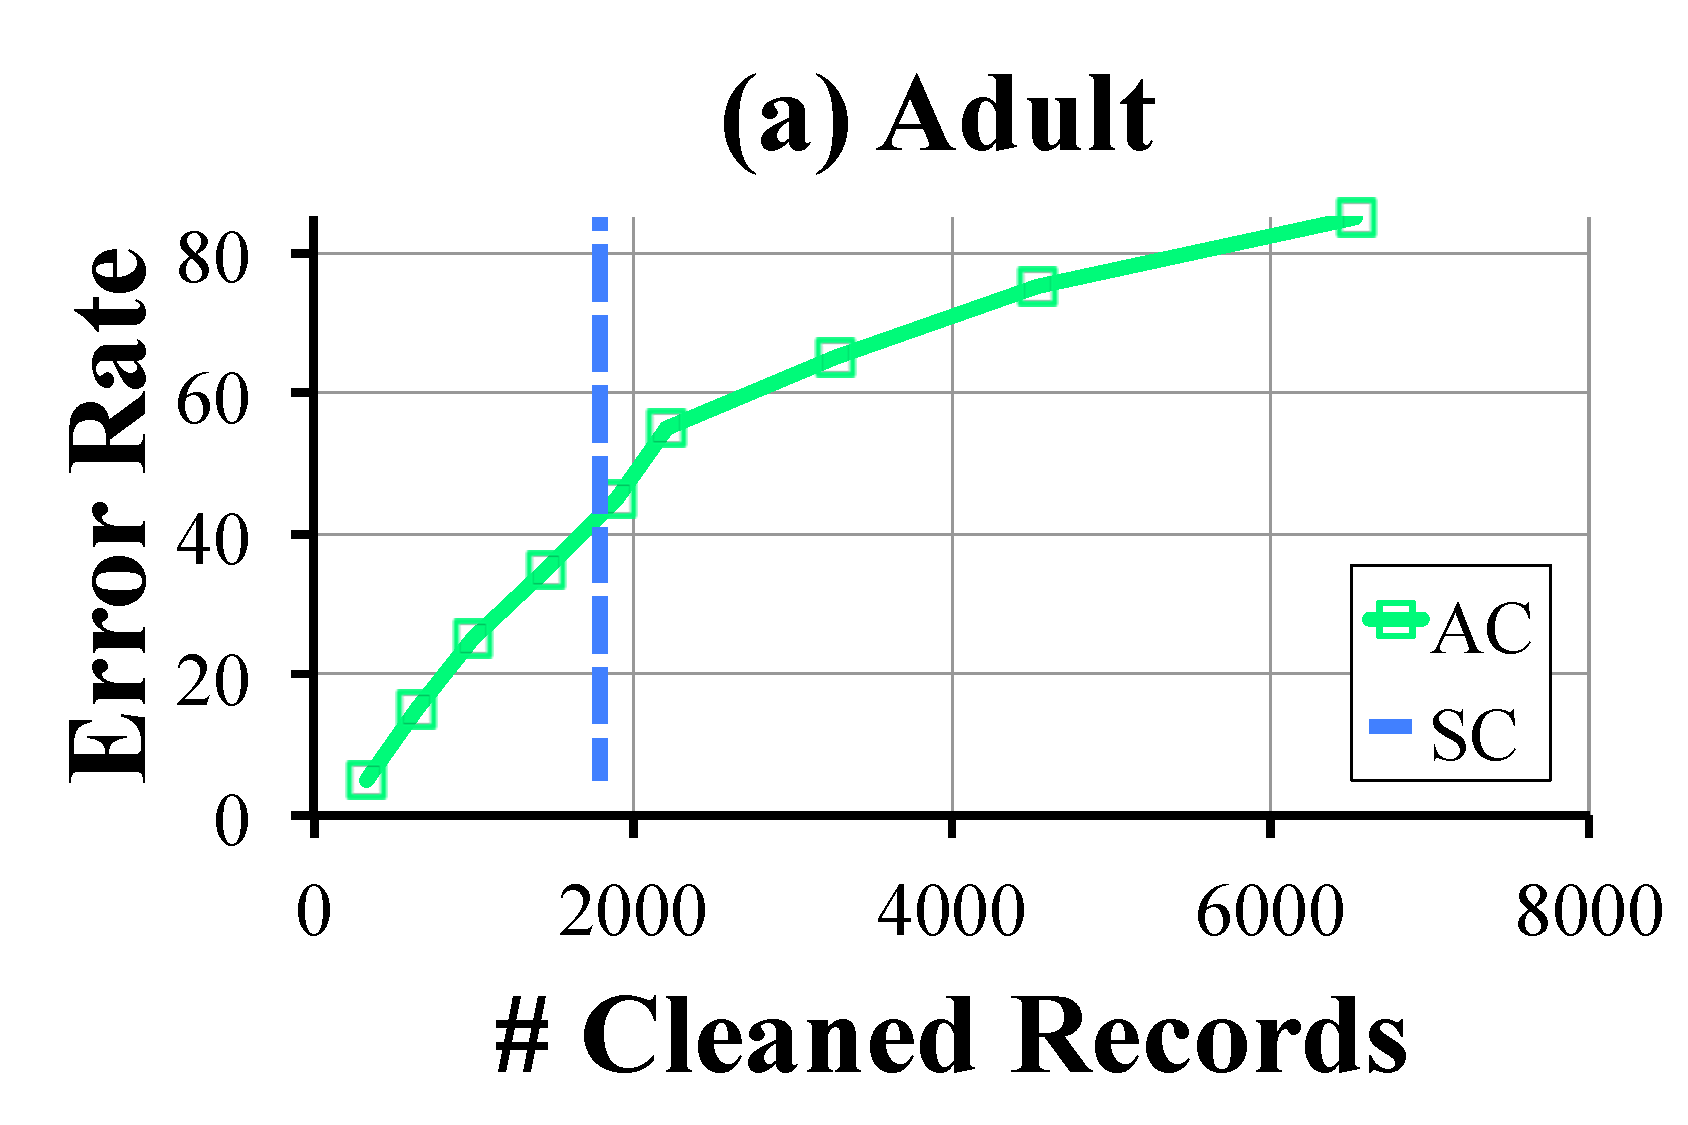
\includegraphics[width=0.49\columnwidth]{exp/exp9a.pdf}
  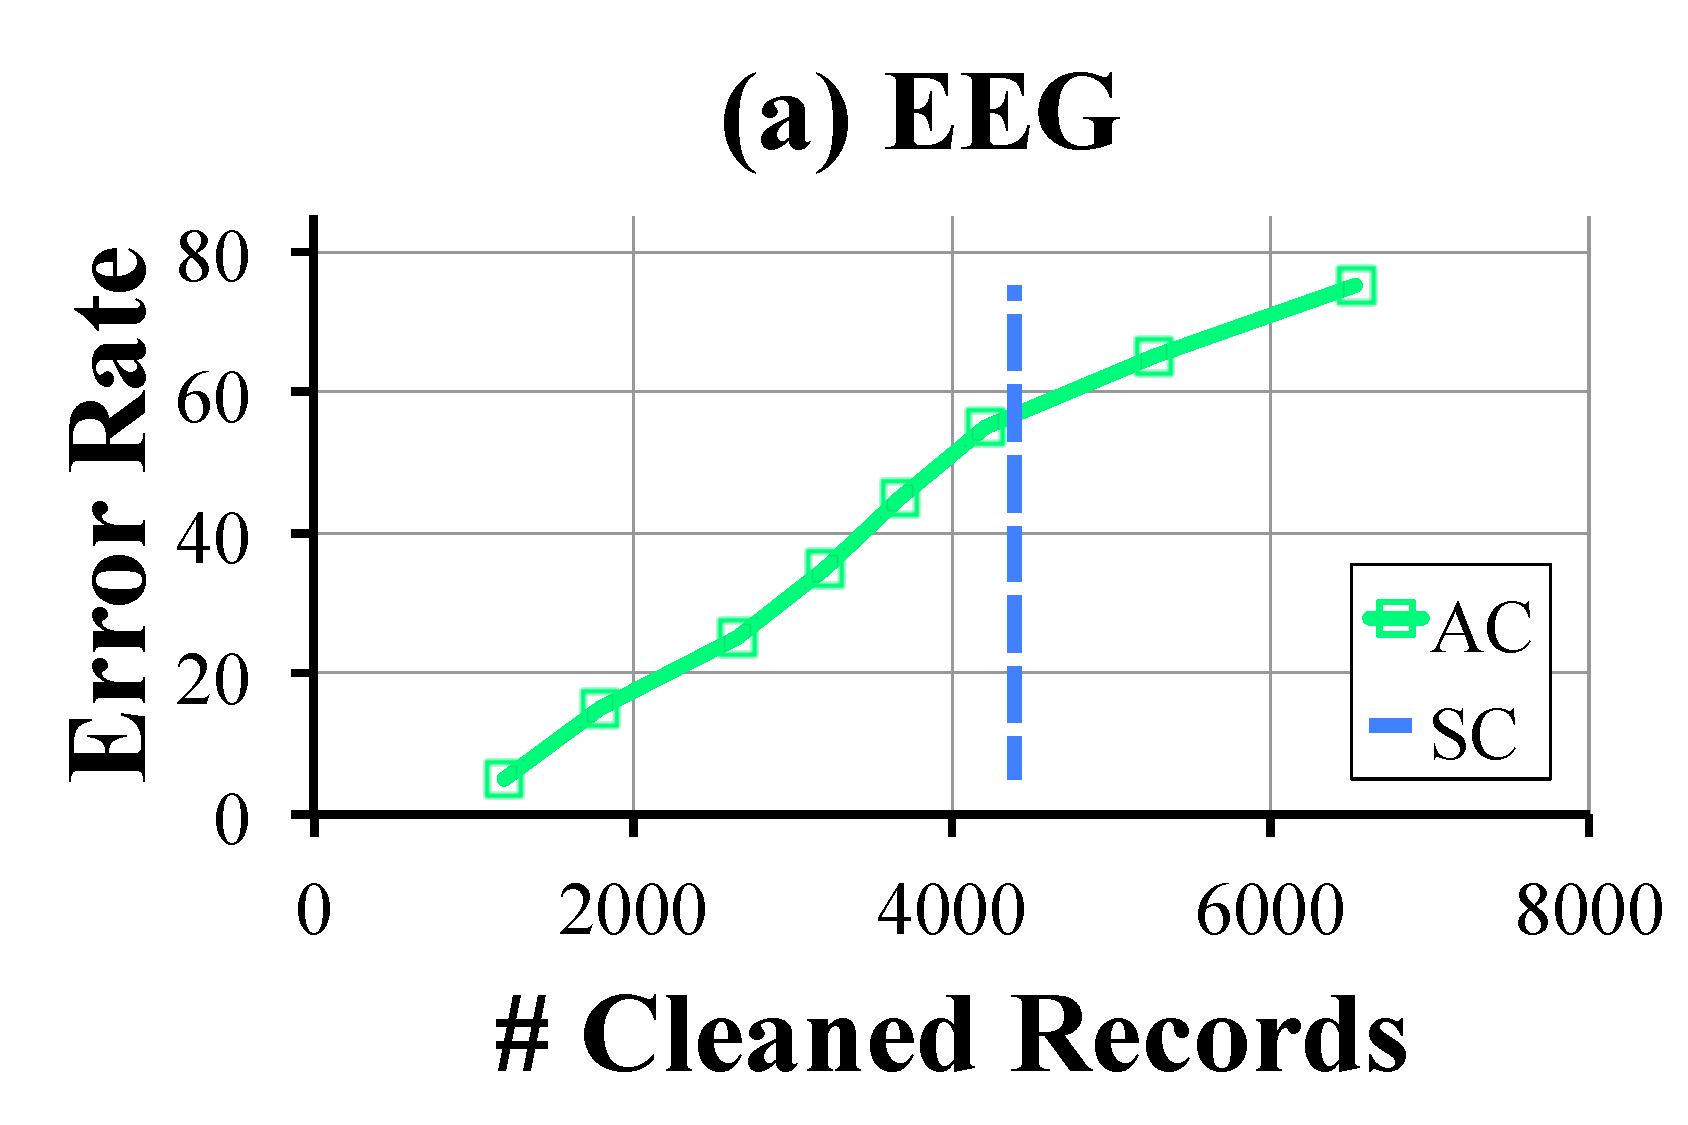
\includegraphics[width=0.49\columnwidth]{exp/exp9b.pdf}
 \caption{\sys performs well until the corruption is so severe that the dirty model is not a good initialization.  \label{bias}}
\end{figure}

\subsection{Adaptive Detection}
In this experiment, we explore how the results of the previous experiment change when we use an adaptive detector rather than the a priori detector.
Recall, in our systematic corruption, we corrupted 3 of the most informative features at random, thus we group these problems into 3 classes.
We use an all-versus-one SVM to learn the categorization.

\subsubsection{Basic Performance}
In Figure \ref{pred-perf}, we overlay the convergence plots in the previous experiments with a curve (denoted by AC+C) that represents \sys using a classifier instead of the a priori detection.
We find an interesting tradeoff where initially \sys is comparable to Active Learning, as our classifier becomes more effective the detection improves the performance.
For both datasets, after cleaning 1000 records, \sys is within 10\% of a priori detection performance.

\vspace{0.25em}

\noindent \emph{Summary: \sys with a classifier converges faster than Active Learning and SampleClean.}

\begin{figure}[t]
\centering
 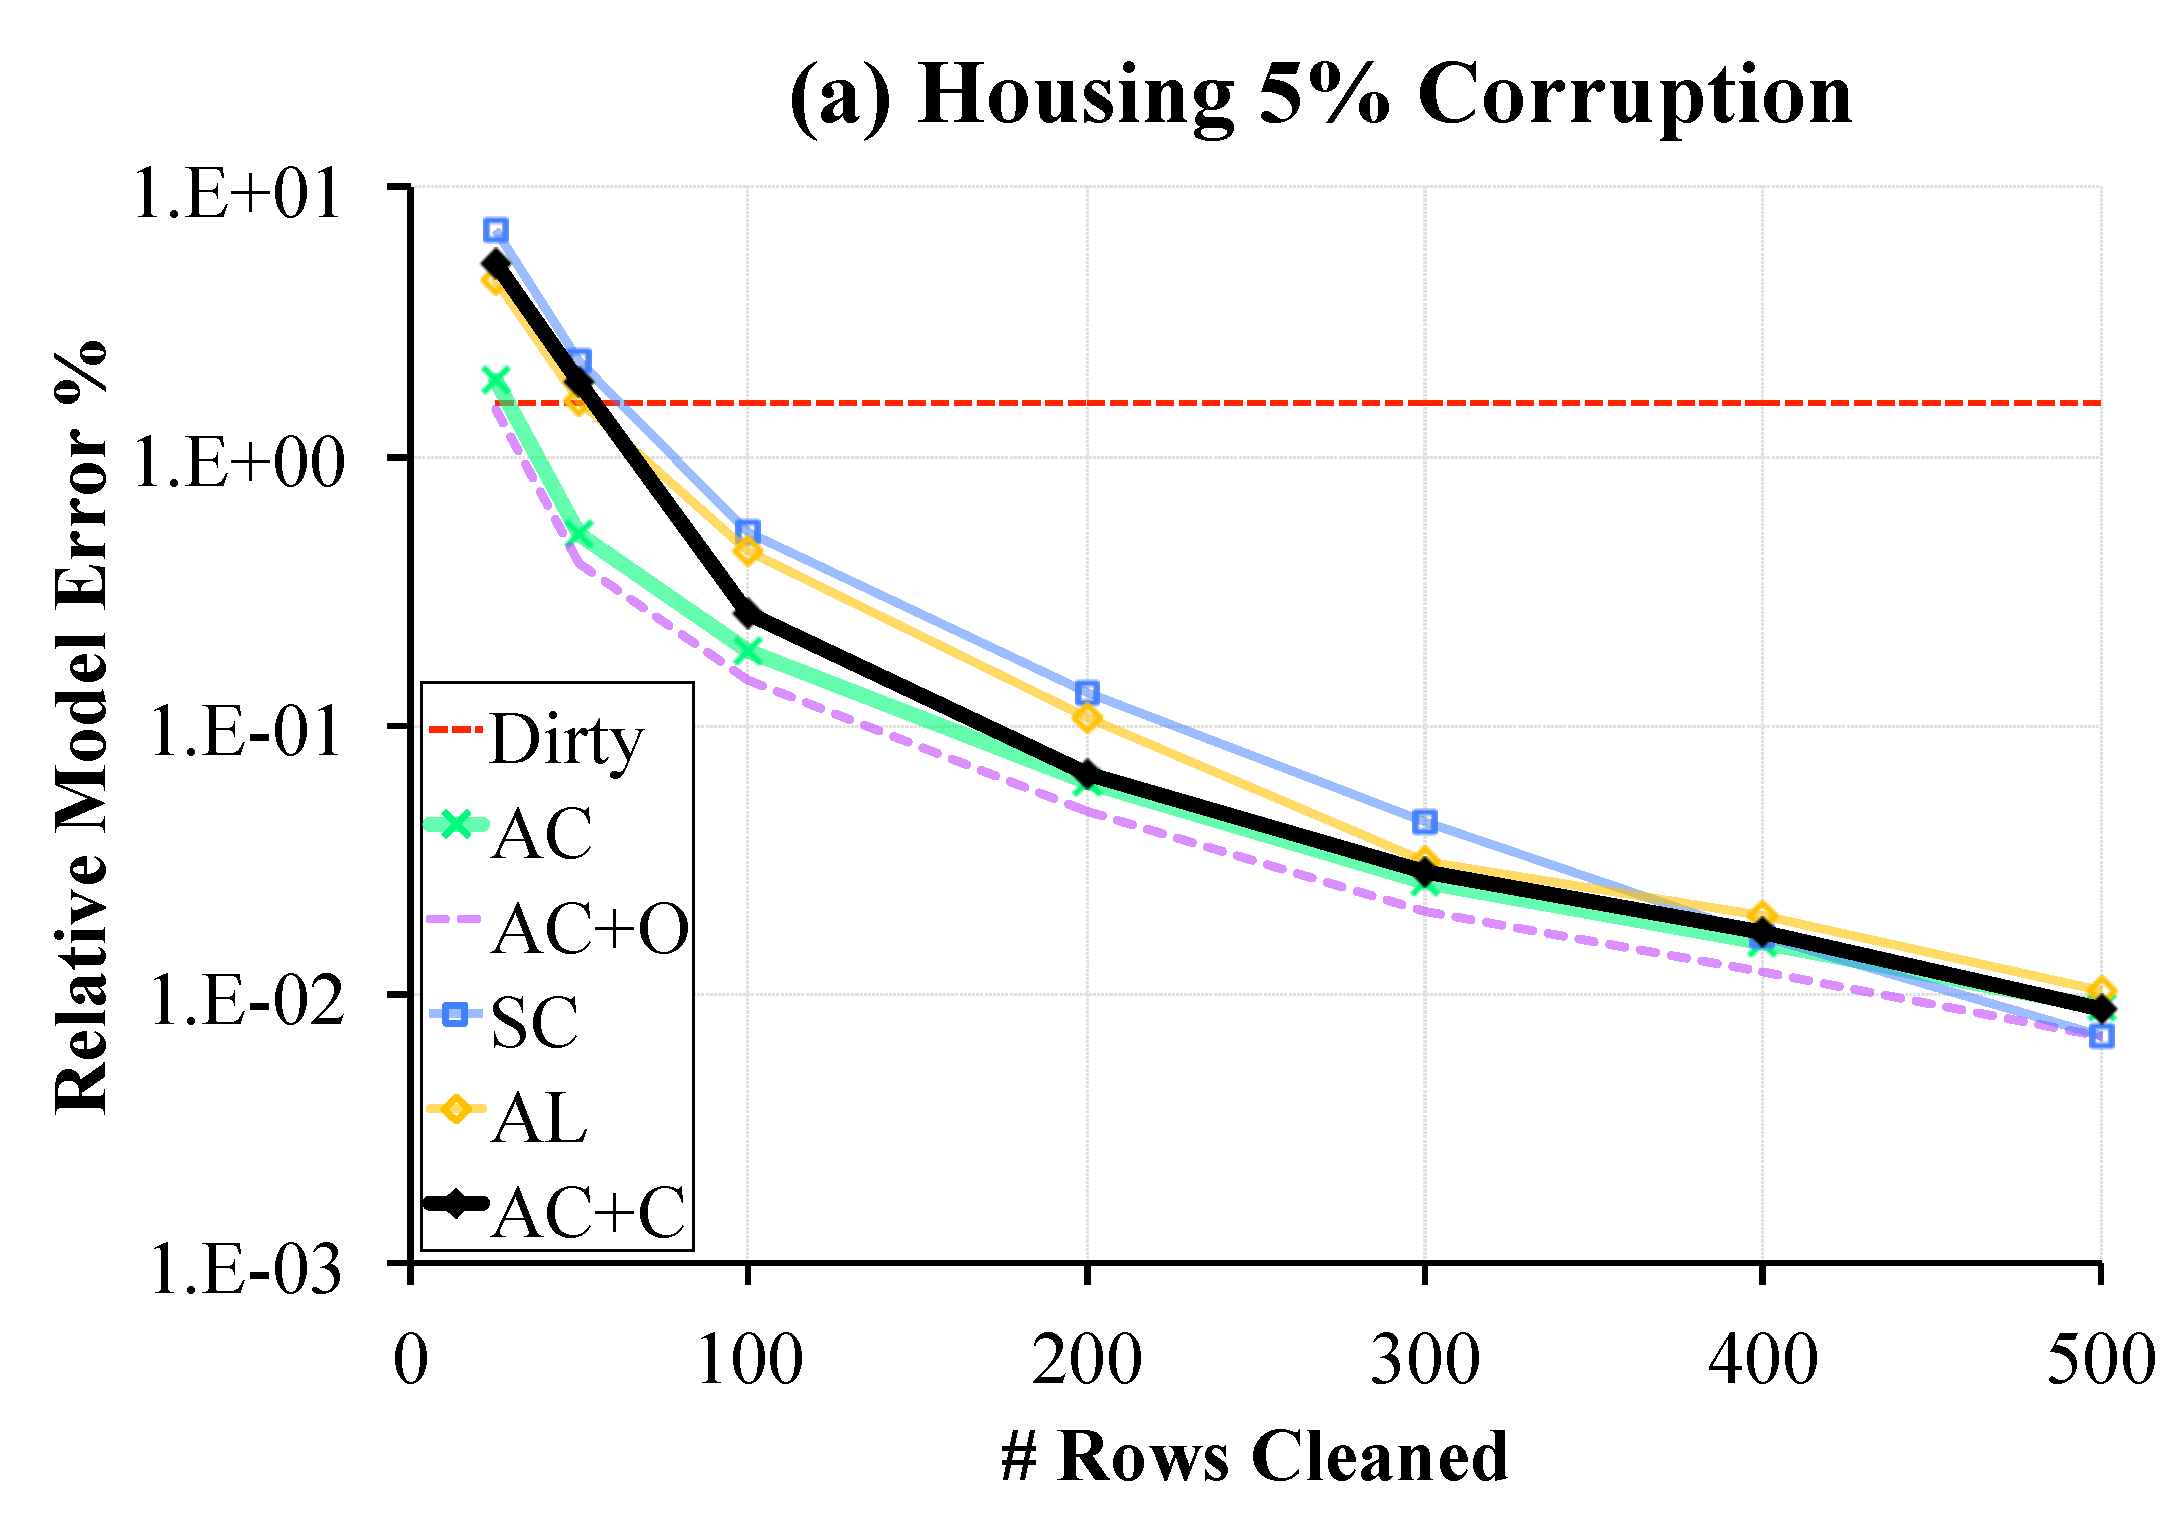
\includegraphics[width=0.49\columnwidth]{exp/exp11a.pdf}
 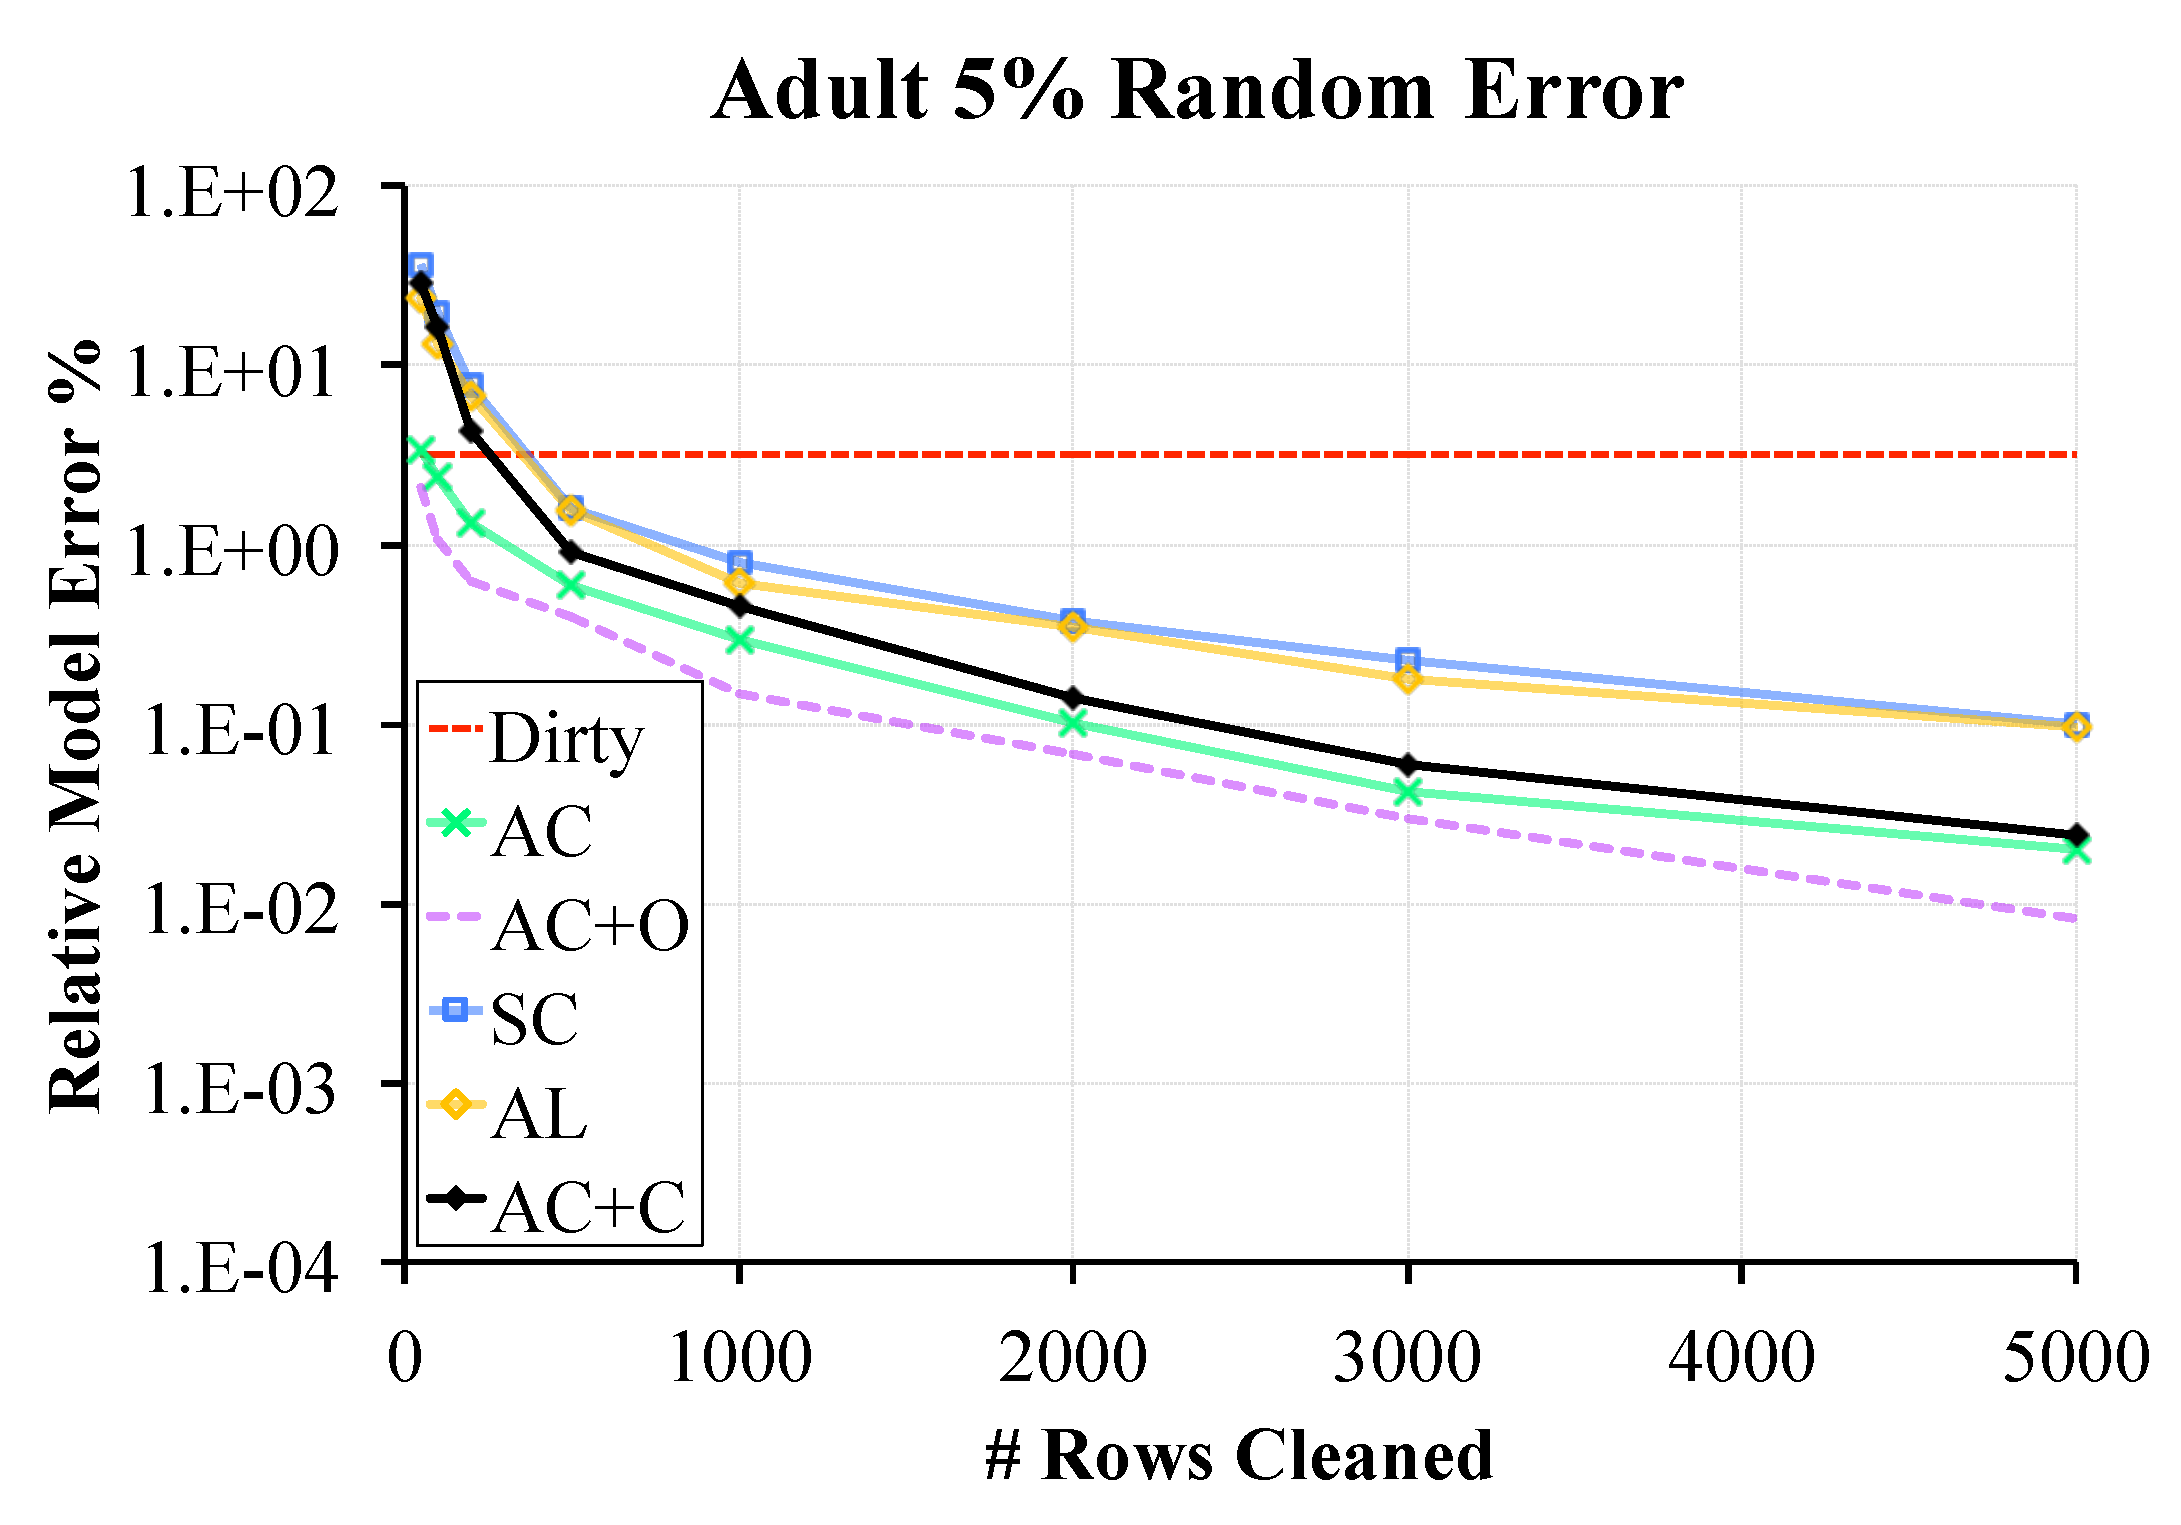
\includegraphics[width=0.49\columnwidth]{exp/exp11b.pdf}
 \caption{Even with a classifier \sys converges faster than Active Learning and SampleClean. \label{pred-perf}}
\end{figure}

\subsubsection{Classifiable Errors}
The adaptive case depends on being able to predict corrupted records.
For example, random corruption that look like other data may be hard to learn.
As corruption becomes more random, the classifier becomes increasingly erroneous.
We run an experiment where we start with the systematic corruption described earlier.
We increasingly make this corruption more random.
Instead of selecting the highest valued records for the most valuable features, we corrupt random records with probability $p$. 
We compare these results to AC-D where we do not have a detector at all at one vertical slice of the previous plot (cleaning 1000 records).
In Figure \ref{tradeoffs2}, we plot the relative error reduction using a classifier.
We find that when the corruption is about 50\% random then we reach a break even point.

\vspace{0.25em}

\noindent \emph{Summary: The adaptive detection can tolerate some misclassifications and still provides improvements until corruption is very random. }

\begin{figure}[ht!]
\vspace{-1em}
\centering
 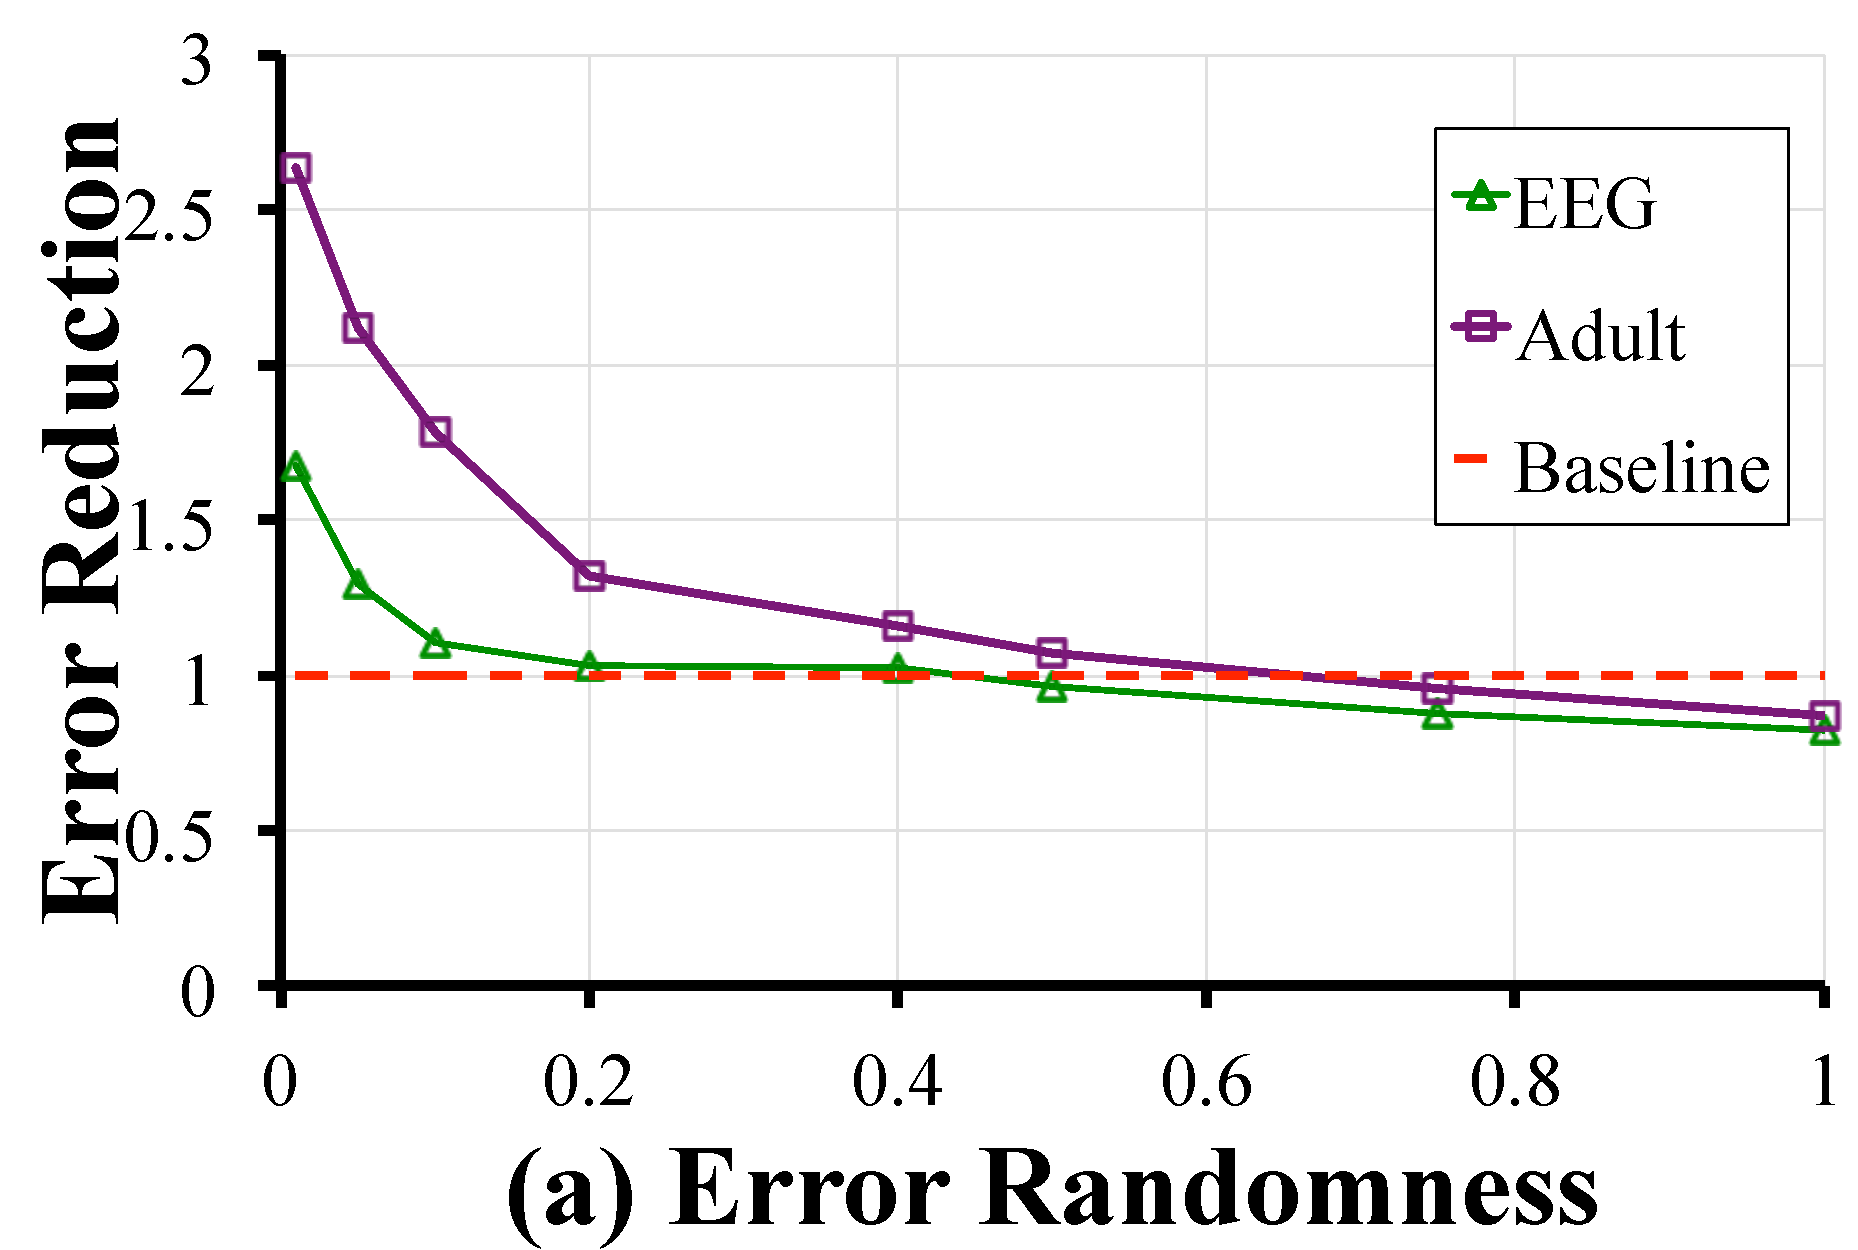
\includegraphics[width=0.49\columnwidth]{exp/exp5a.pdf}
 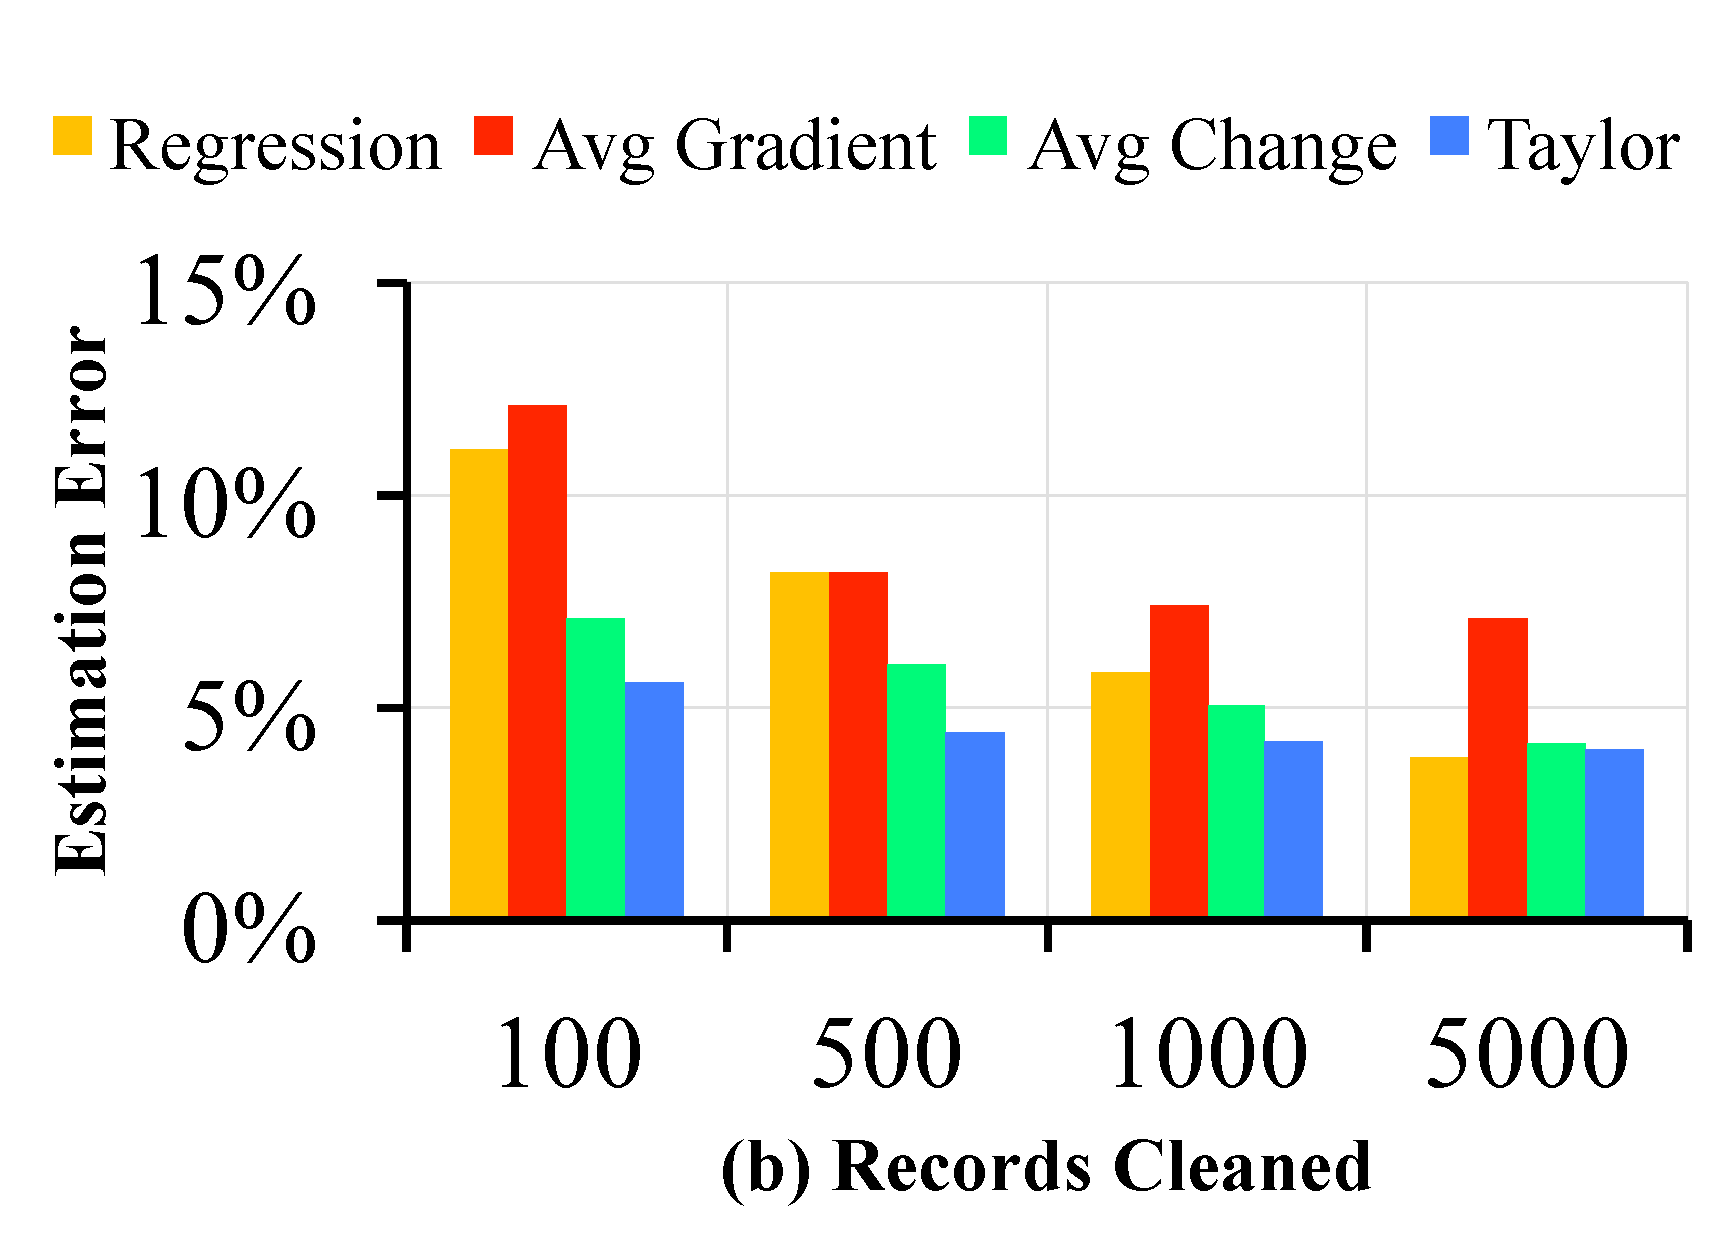
\includegraphics[width=0.49\columnwidth]{exp/exp12.pdf}
 \caption{(a) Data corruptions that are less random are easier to classify, and lead to more significant reductions in relative model error. (b) The Taylor series approximation gives more accurate estimates when the amount of cleaned data is small. \label{tradeoffs2}}
\end{figure}

\subsection{Estimation}\label{est}
In Figure \ref{tradeoffs2}b, we explore how estimation technique performs compared to a few alternative estimation techniques: (1) ``linear regression" where we train a linear regression model that predicts the clean gradient as a function of the dirty gradient, (2) ``average gradient" change where we do not use the detection to inform how to apply the estimate, (3) ``average feature change" where we do not linearize but use detection, and (4) our taylor series linear approximation.
We only how accurately the technique can estimate the gradient for sampling.
More accurate gradient estimates will result in faster convergence.

Using the EEG dataset, we measure the relative estimation error (relative L2 error with the true gradient) for different amounts of data cleaned.
The Taylor series approximation proposed in this work gives more accurate for small cleaning sizes.
We give the intuition in Section \ref{acc} where the linearization prevents amplification of errors due to quadratic terms.
Linear regression and the average feature change technique do eventually perform comparably but only after cleaning much more data.

\vspace{0.25em}

\noindent \emph{Summary: Linearized gradient estimates are more accurate when estimated from small samples. }

\subsection{Real Scenarios}
We evaluate \sys in two real scenarios, one demonstrating the a priori case and one for the adaptive detection case.

\subsubsection{A Priori: Constraint Cleaning}\label{dfd-exp}
In our first real scenario, we explore the Dollars for Docs dataset published by Pro Publica that we described throughout the paper.
We treat this problem as a constraint-based cleaning problem where we encode these problems as data quality constraints (see Appendix \ref{dfd-errors} for constraints and example errors). 
This provides us with a detector for the corruption. 
To fix the detected violations, we manually cleaned data.
We confirmed drug names with company catalogs and used judgement to make the labels consistent.
To run this experiment, we manually cleaned the entire dataset up front, and simulated sampling from the dirty data and cleaning by looking up the value in the cleaned data.
Figure \ref{dfd}a shows that \sys converges faster than Active Learning and SampleClean.
To achieve a 4\% relative error (i.e., a 75\% error reduction from the dirty model), \sys cleans 40000 fewer records than Active Learning.
Also, for 10000 records cleaned, \sys has 3.5x smaller error than SampleClean.

Figure \ref{dfd}b shows the true positive rate (fractiion of non-covered research contributions identified) of the classifier as a function of the number of records cleaned. 
We find that on the dirty data, we can only classify 66\% of the positive examples correctly.
On the cleaned data, this classifier is nearly perfect with a 97\% true positive rate.
\sys converges to the cleaned accuracy faster than the alternatives.

\vspace{0.25em}

\noindent \emph{Summary: In a real a priori detection scenario, \sys significantly reduces the number of records to clean to train an accurate model. }

\begin{figure}[ht!]
\centering
 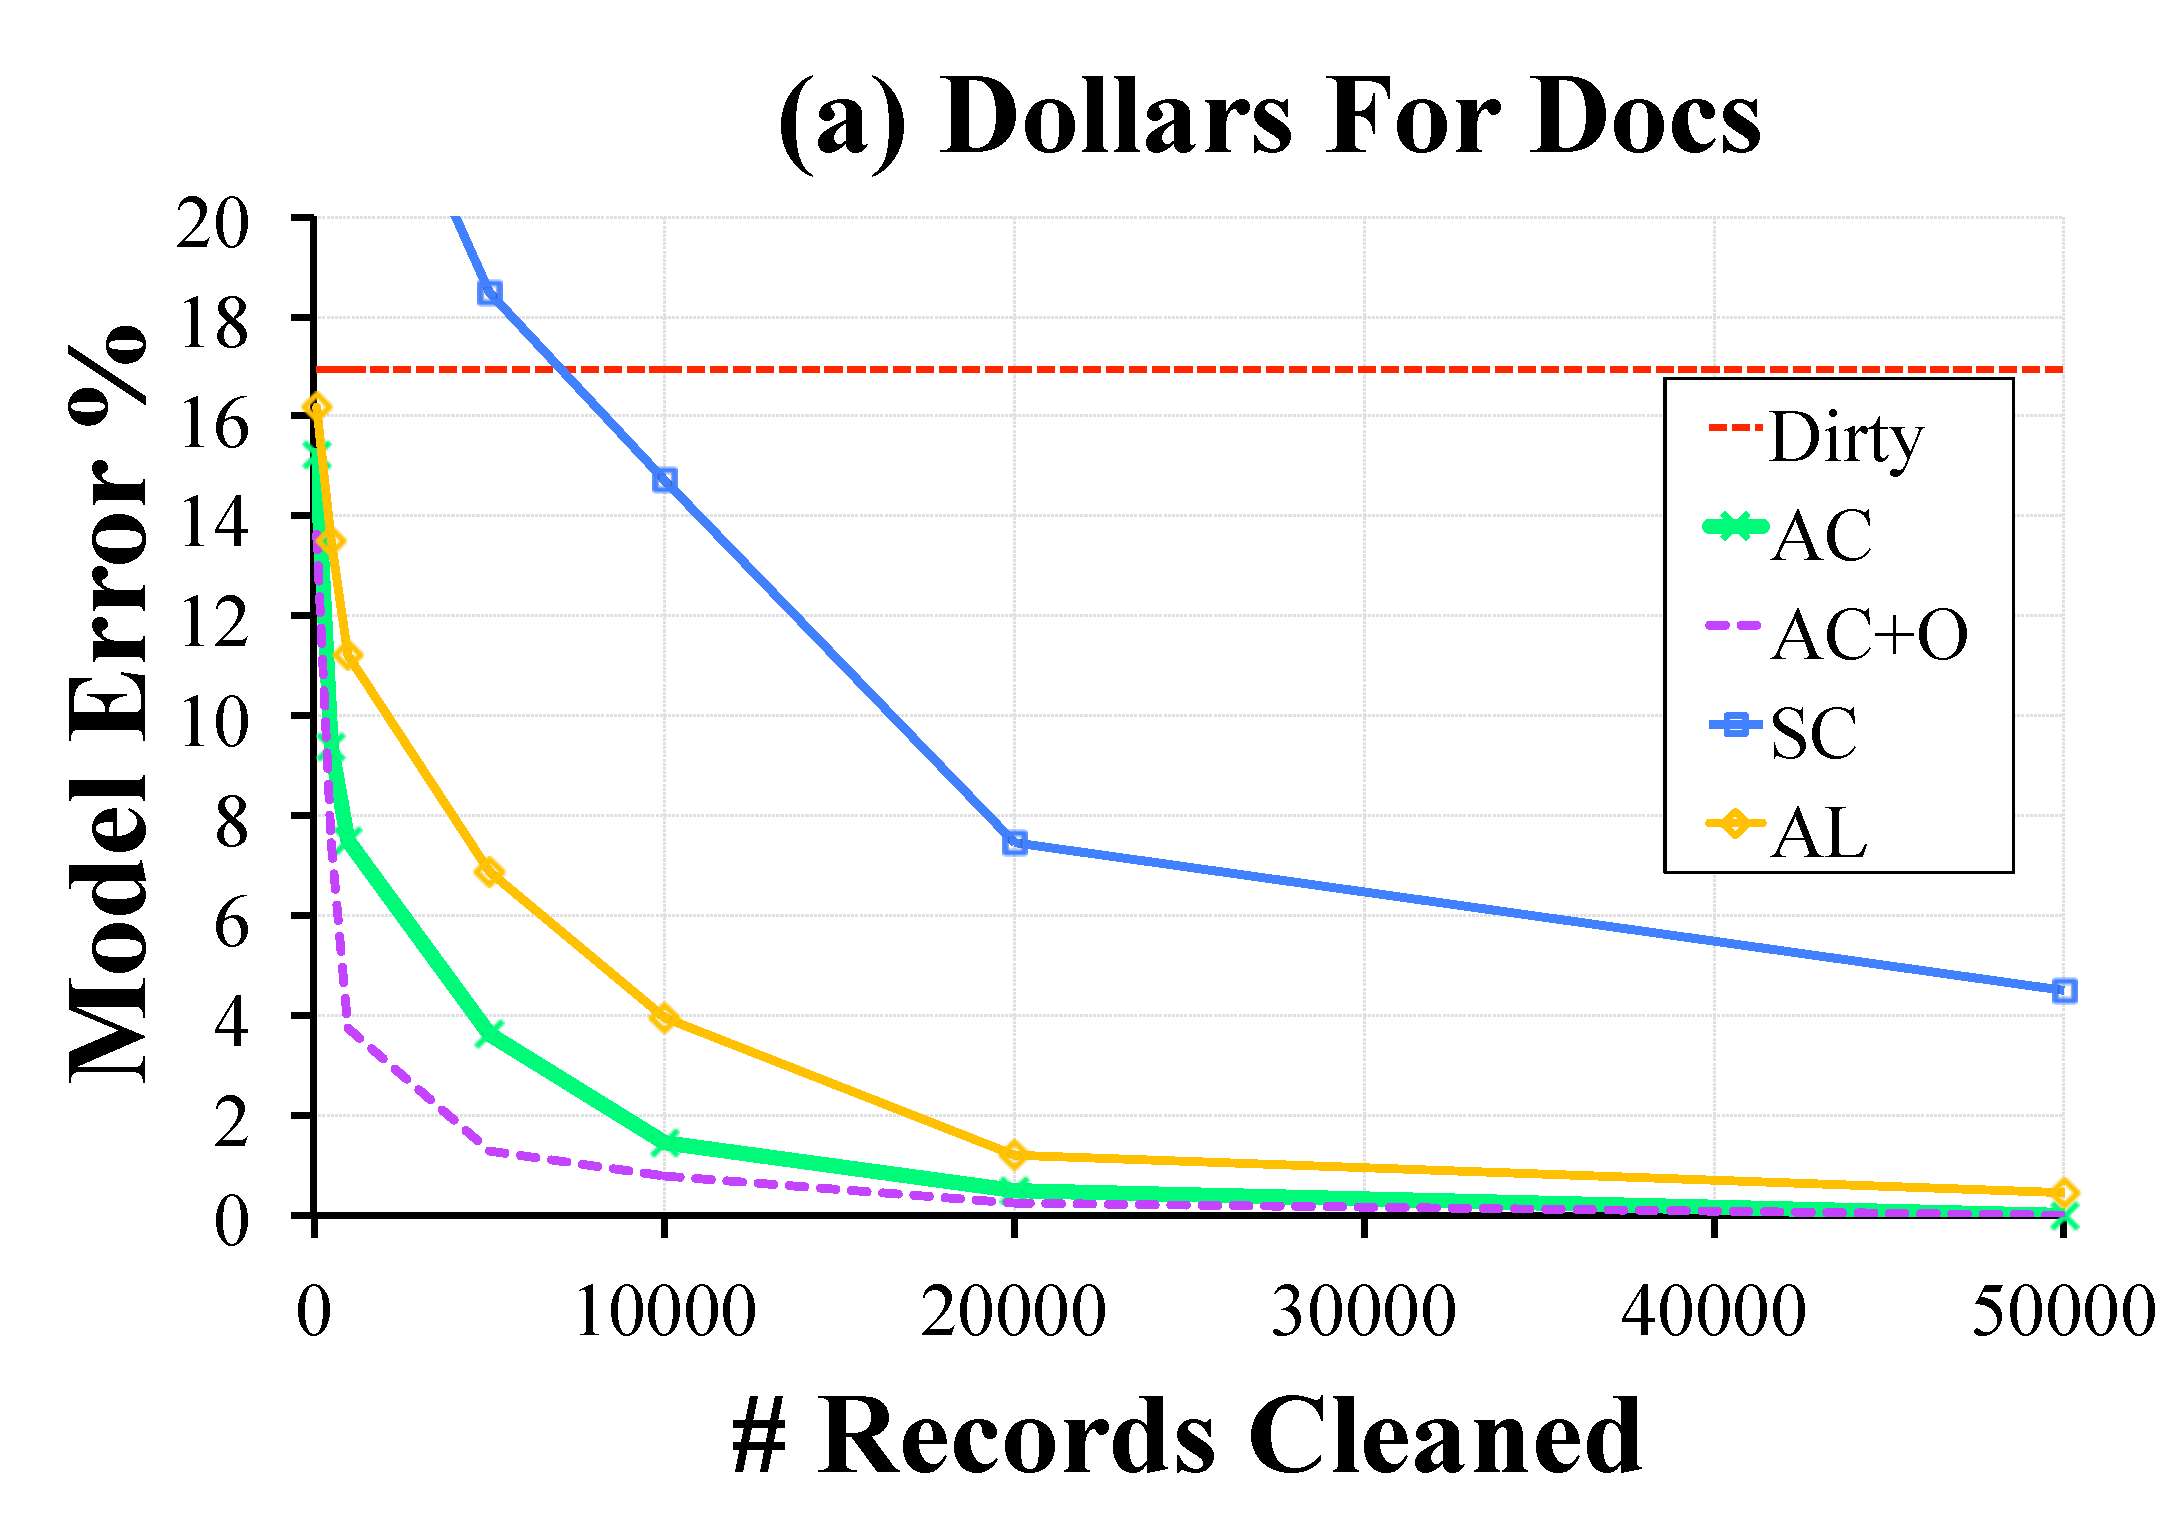
\includegraphics[width=0.49\columnwidth]{exp/exp13a.pdf}
 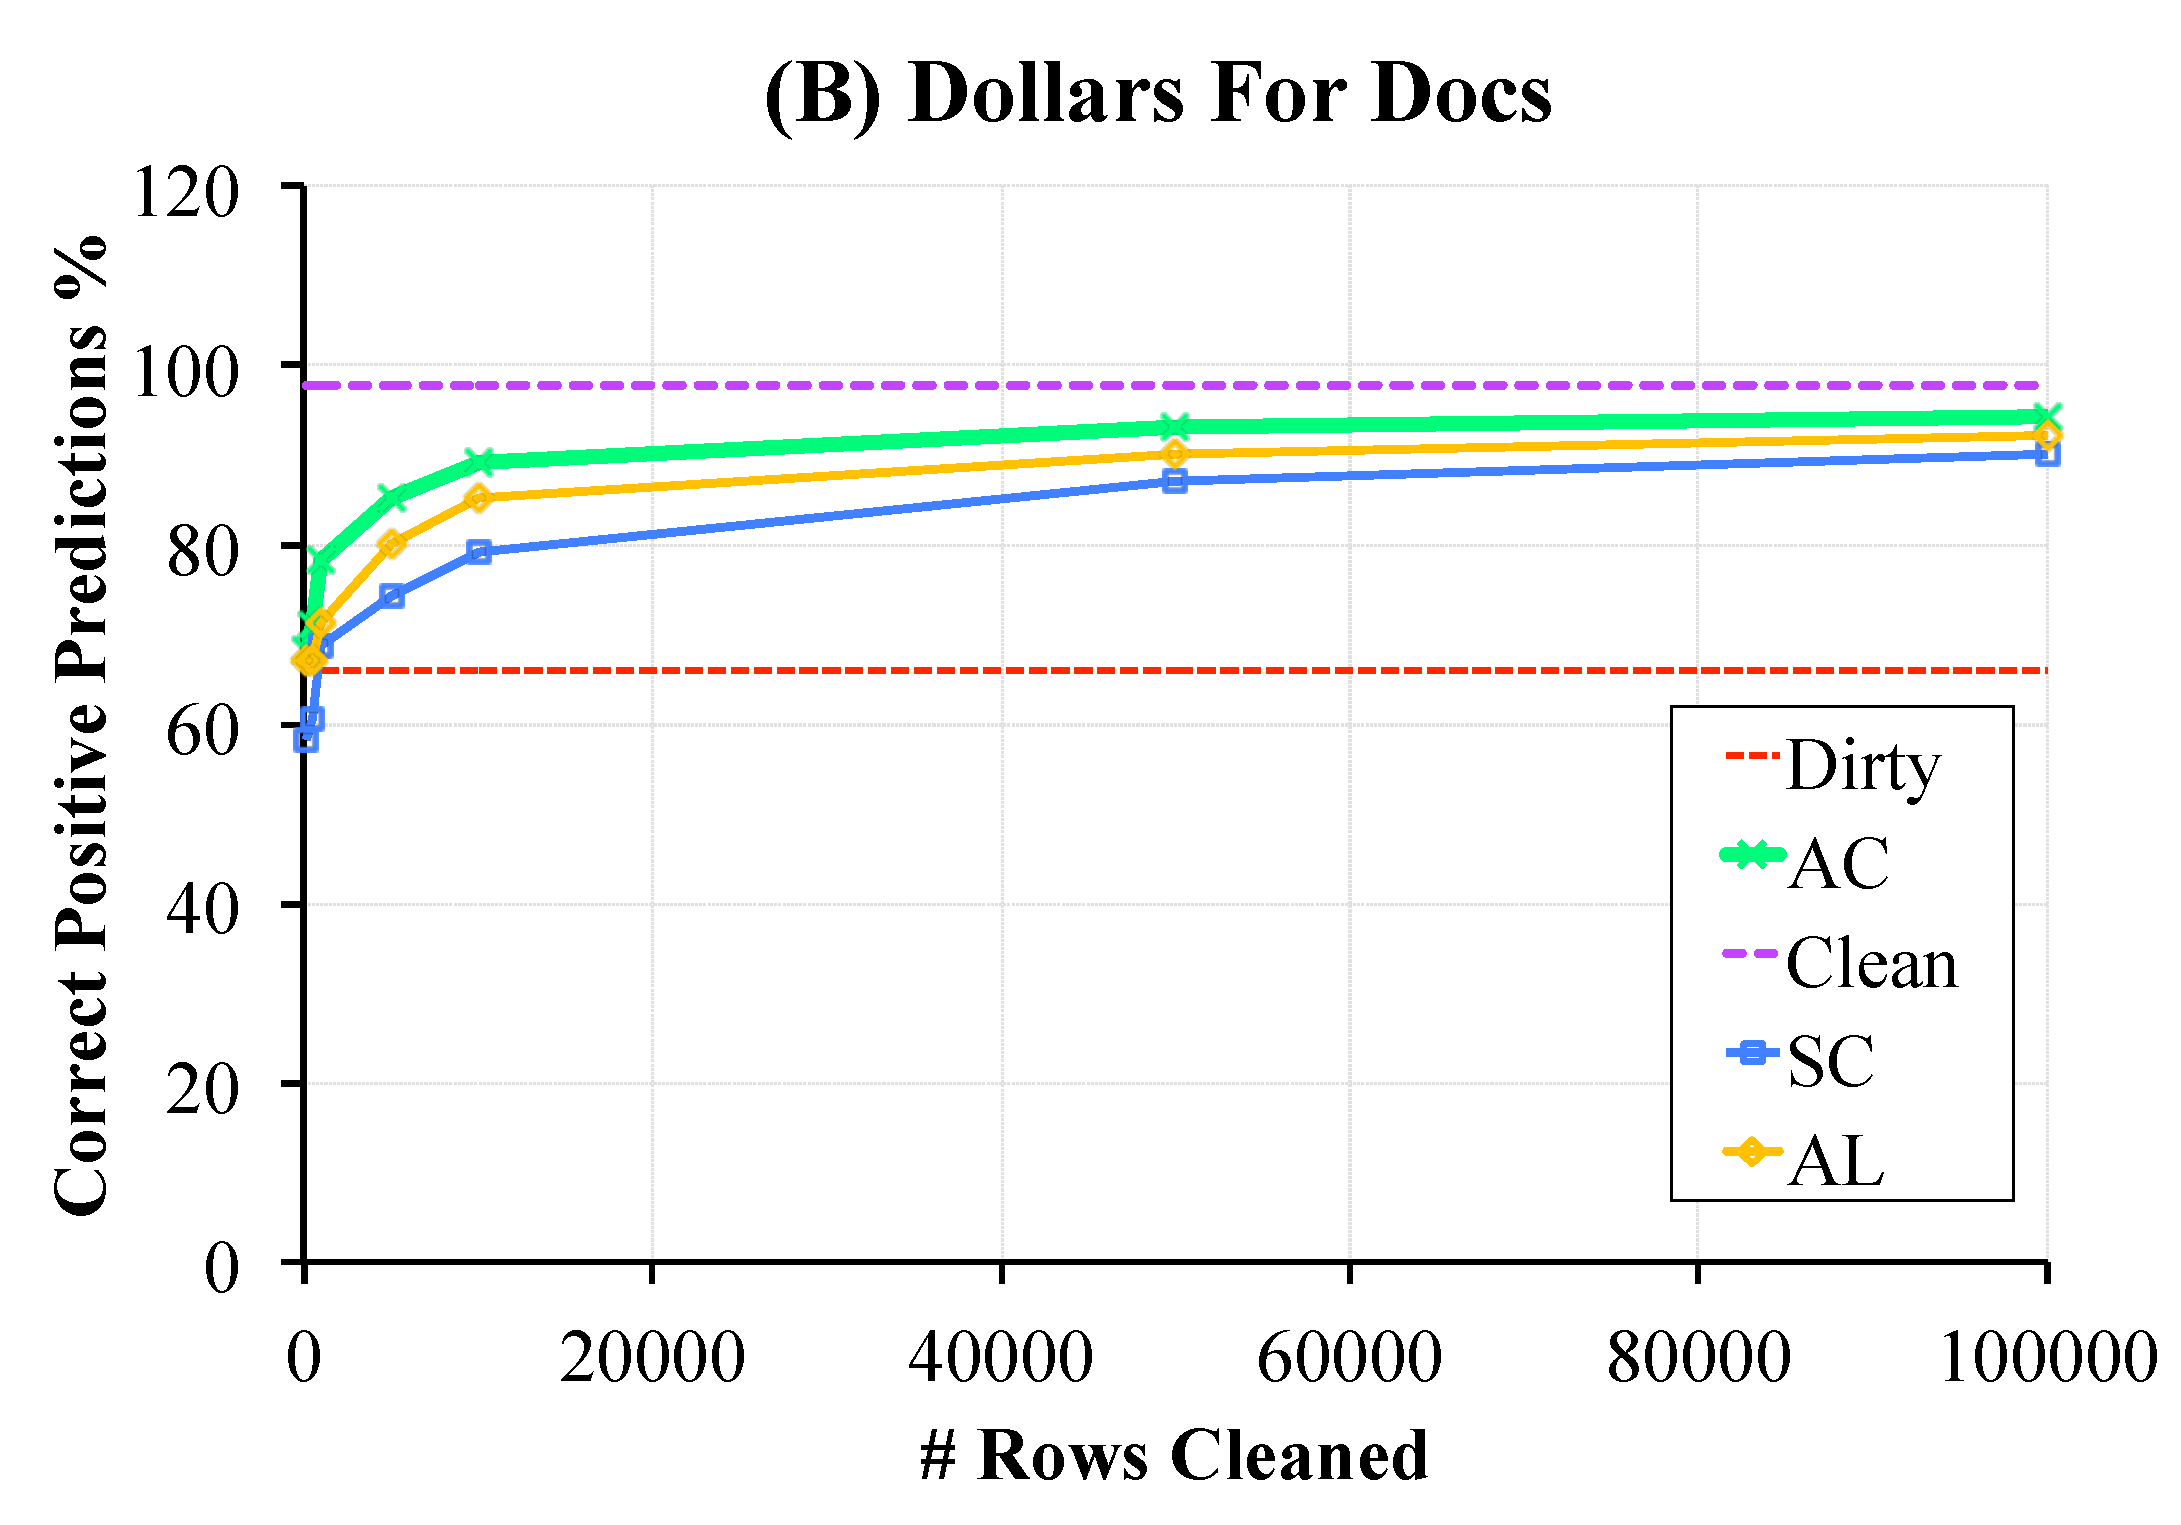
\includegraphics[width=0.49\columnwidth]{exp/exp13b.pdf}
 \caption{(A) The relative model error as a function of the number of cleaned records. (B) The true postive rate as a function of the number of cleaned records. \label{dfd}}
\end{figure}

\subsubsection{Adaptive: Replacing Corrupted Data}
We consider the following scenario with the MNIST handwritten digit recognition dataset.
Suppose, our goal is to classify digits into a set of classes.
However, we suspect that some of our raw images are of low quality.
Typicaly image processing workflows are long with many different featurization steps.
As a result, changes to the raw images may have very significant effects on some features.
In this scenario, the analyst must inspect a potentially corrupted image and replace it with a higher quality one.
We devise an ``adaptive detection" \sys scenario for this example.

The MNIST dataset consists of 64x64 grayscale images.
We run two experiments, in which we have two types of corruptions: (1) 5x5 block removal where take a random 5x5 block from the image and set its pixel values to 0, and (2) Fuzzy where we run a 4x4 moving average over the entire image.
We applied these corruptions to a random 5\% of the images.
We constructed these corruptions to mimic the random vs. systematic corruption that we studied before.
The 5x5 block removal behaves much more like a systematic corruption. 
Typical image processing features are based on edges and corrupting edges leads to ambiguities.
On the other hand, the making the image fuzzy is more like a random corruption.
We use a 9 class classifier (one for each digit) to detect the corruption.


\iffalse
\begin{figure}[ht]
\centering
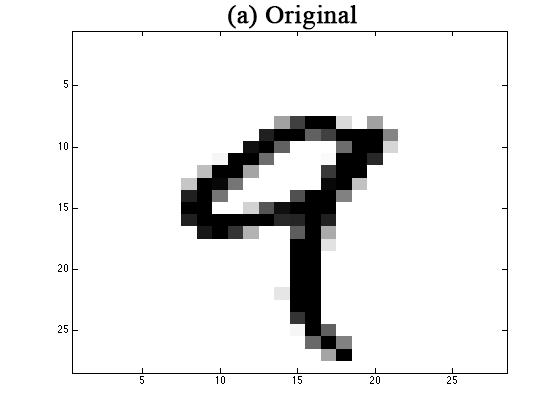
\includegraphics[scale=0.20]{exp/original.png}
 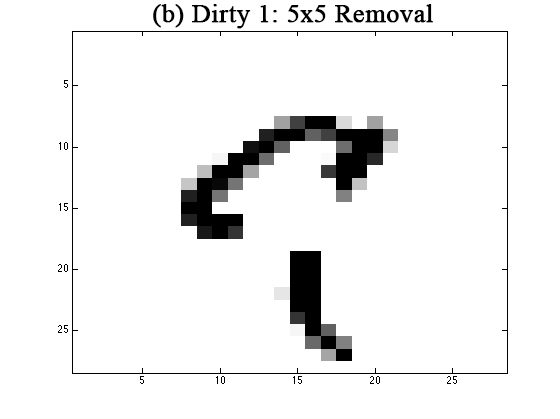
\includegraphics[scale=0.20]{exp/5x5removal.png}
 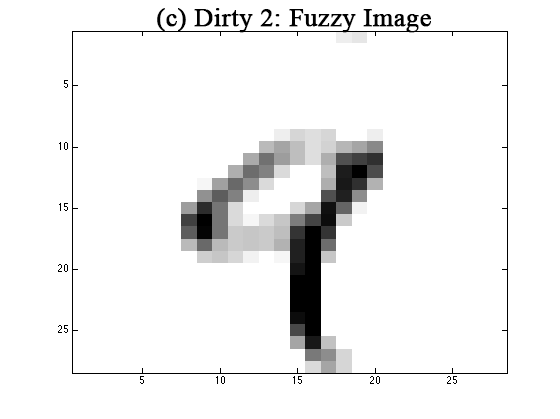
\includegraphics[scale=0.20]{exp/fuzzy.png}
 \caption{We experiment with two forms of corruption in the MNIST image datasets: 5x5 block removal and making the images fuzzy. Image (a) shows an uncorrupted ``9", image (b) shows one corrupted with block removal, and image (c) shows one that is corrupted with fuzziness. \label{mnist-corr}}
\end{figure}
\fi

Figure \ref{mnist} shows that \sys makes more progress towards the clean model with a smaller number of examples cleaned.
To achieve a 2\% error for the block removal, we can inspect 2200 fewer images than Active Learning and 2750 fewer images than SampleCLean.
For the fuzzy images, both Active Learning and \sys reach 2\% error after cleaning fewer than 100 images, while SampleClean requires 1750.

\vspace{0.25em}

\noindent \emph{Summary: In a real adaptive detection scenario, \sys significantly reduces the number of records to clean to train an accurate model. }

\begin{figure}[ht]
\centering
 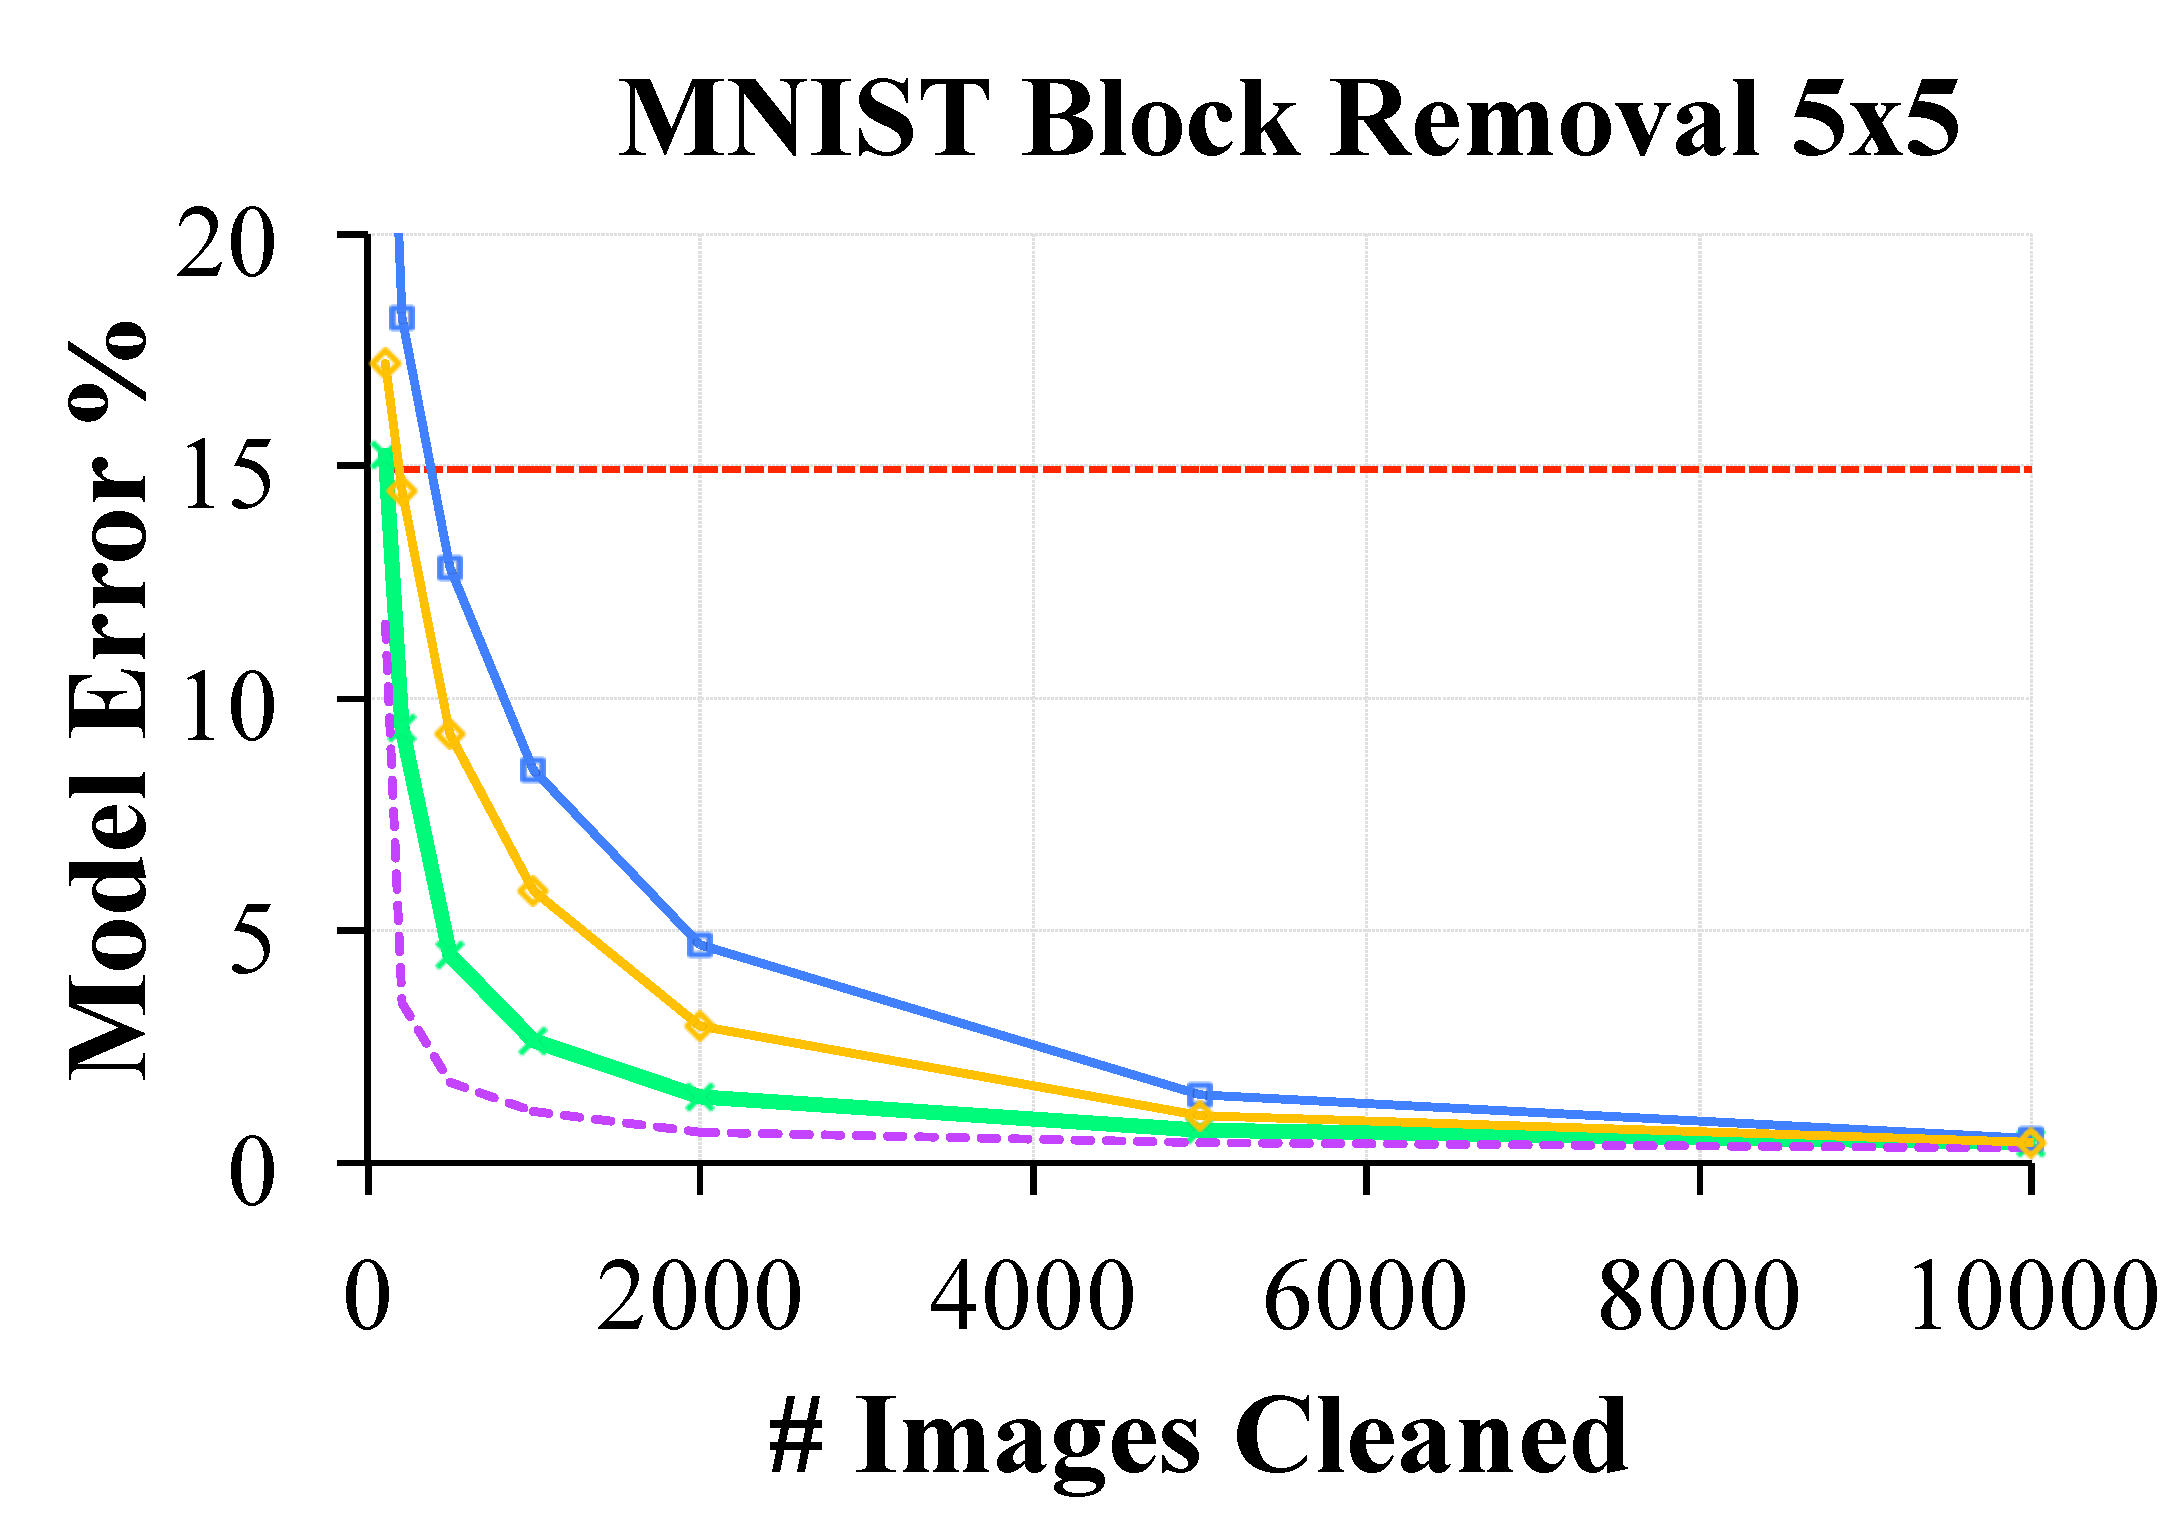
\includegraphics[width=0.49\columnwidth]{exp/exp7a.pdf}
 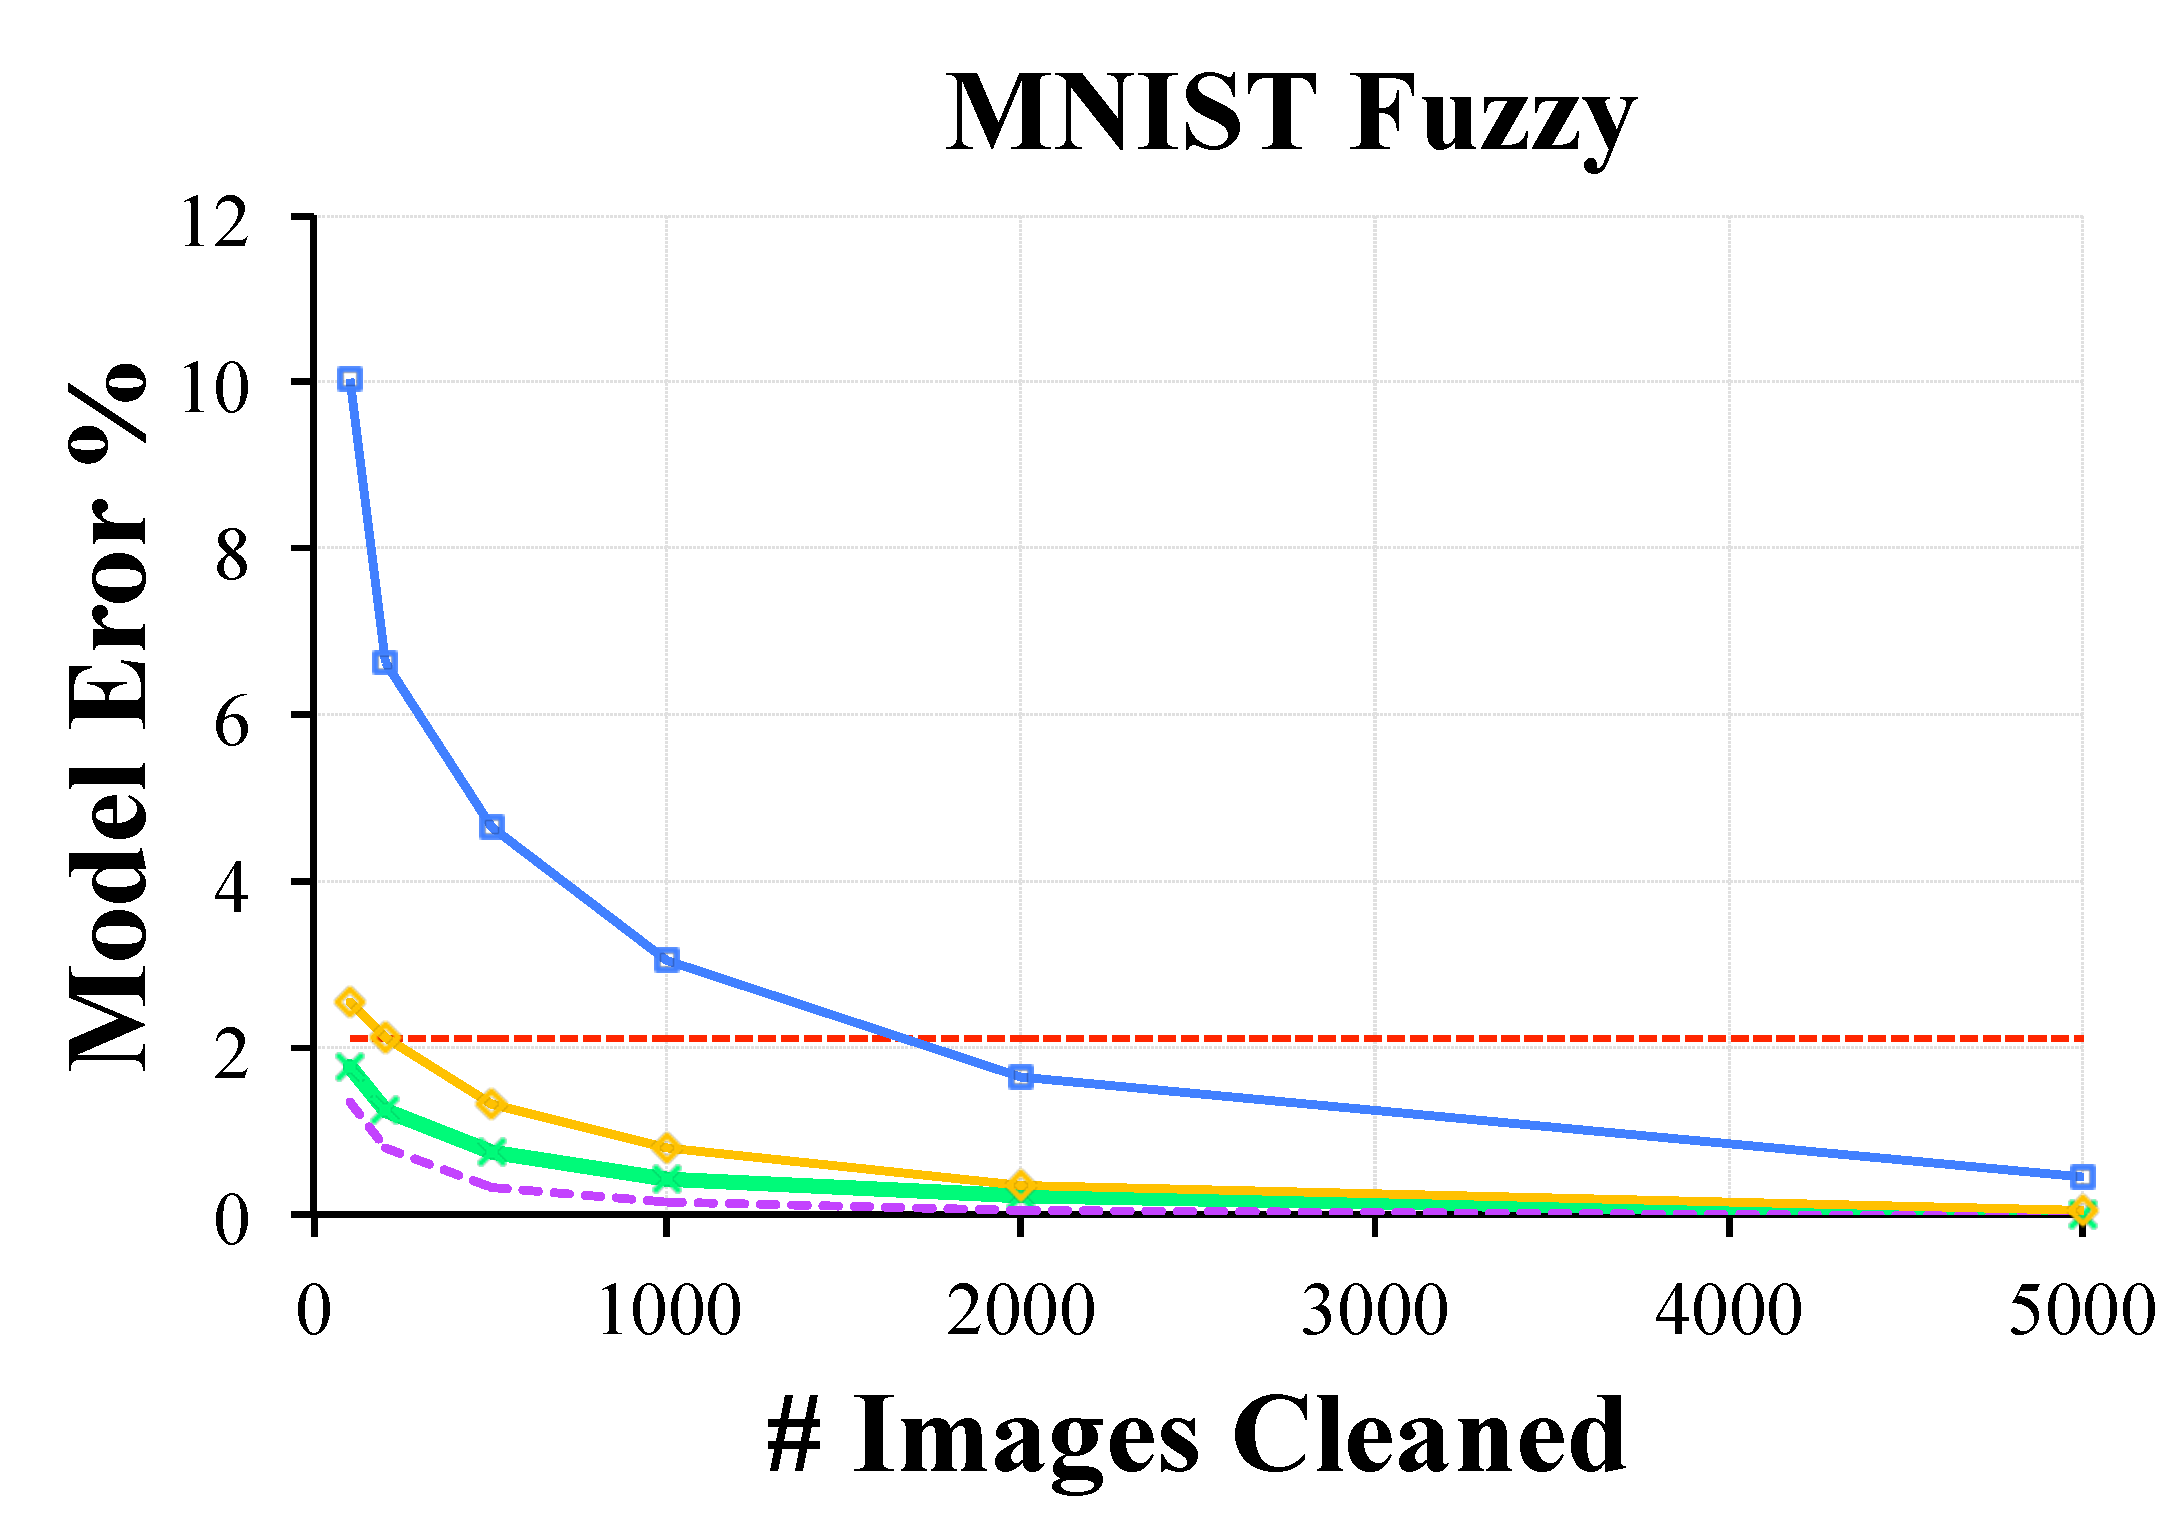
\includegraphics[width=0.49\columnwidth]{exp/exp7b.pdf}
 \caption{In a real adaptive detection scenario with the MNIST dataset, \sys outperforms Active Learning and SampleClean. We simulate systematic corruptions with image block removal and random corruptions with image fuzzying.  \label{mnist}}
\end{figure}
